\documentclass{beamer}	
\mode<presentation>
 
\usepackage{pdfpages}
\usepackage{fancyvrb}
\usepackage{chemarr}

\usepackage{amsmath}		%% mathematics typesetting
\usepackage{amssymb}
 
\usepackage{epigraph}   %% nice setting of quotations

\usepackage{tabularx} %% allows to use row colours in tables

\usepackage{ulem}

\usepackage{booktabs}

\usepackage{siunitx} %% tpyeset SI units

\usepackage{CJKutf8} %% typeset Chinese characters

\usepackage{pdfpages}%% include pdfs

\usepackage{graphicx}
\usepackage{animate} %% show animated gifs

\DeclareMathAlphabet{\mathcalligra}{T1}{calligra}{m}{n}


% Color and Theme. Can be changed. However, this one's quite nice.
\usetheme{Madrid}
\definecolor{theme}{rgb}{0.84,0,0.21}
\usecolortheme[named=theme]{structure}

%%  Title information
\title[M11.13.6 Visuelles System II]{M11.13.6 Visuelles System II: \\ Retinale Signalverarbeitung und zentrale Sehbahn}
\author[melanie.stefan@medicalschool-berlin.de]{}
\institute[]{Prof. Melanie Stefan \\ melanie.stefan@medicalschool-berlin.de}
\date{WiSe 2023/24}
 

% Table of contents to pop up at the beginning of each section
\AtBeginSection[]
{
  \begin{frame}<beamer>
    \frametitle{Outline}
    \tableofcontents[currentsection,currentsubsection]
  \end{frame}
}
 
\beamertemplatenavigationsymbolsempty

\begin{document}


{ \usebackgroundtemplate{
\includegraphics[width=1.2\paperwidth]{MSB_Titelseite.pdf}} 
\begin{frame}

 \maketitle 

$\,$\\[6cm] 


\end{frame} 
}


%% Hook:

%% Bild Myopia, erste Vorlesung, wie geht es jetzt weiter? 
\begin{frame}{Licht durchquert einen komplizierten optischen Apparat}

\begin{columns}[c]

\begin{column}{5cm}
\begin{center}
    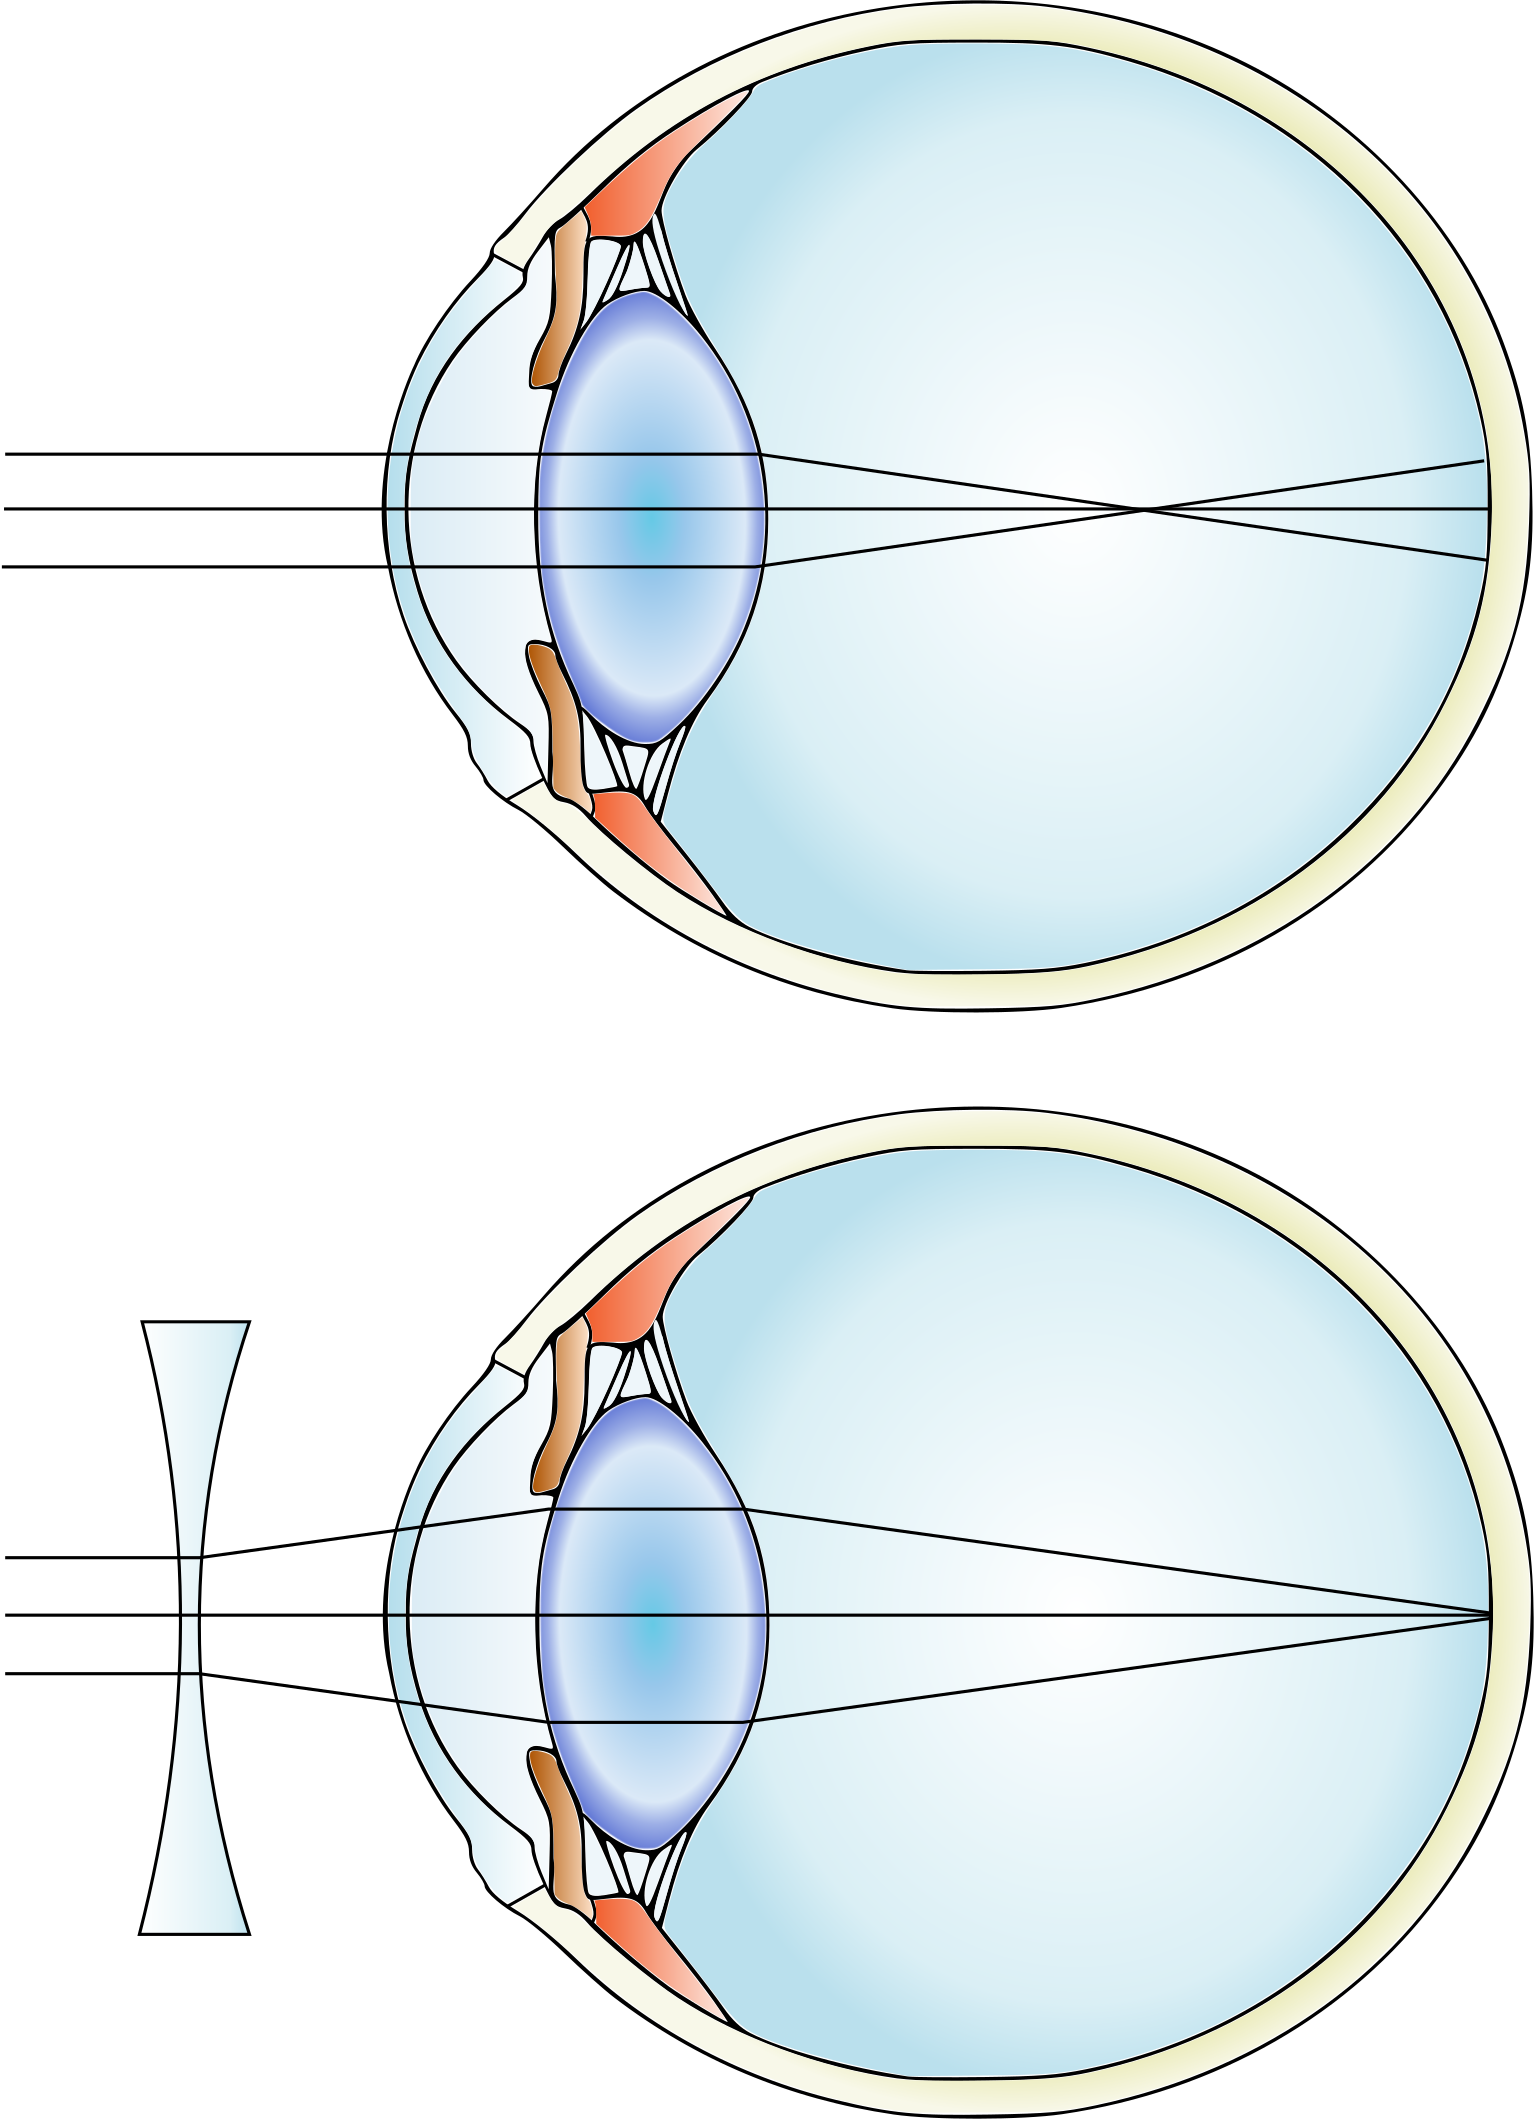
\includegraphics[width=\textwidth]{myopia.png}
\end{center}

\end{column}

\begin{column}{5cm}


\pause

Aber wie gehts weiter?

\end{column}


\end{columns}

    
\end{frame}


 
% %% %% TLIA
\begin{frame}

 \frametitle{In dieser Vorlesung geht es um \dots}

\dots die Sehbahn von den Rezeptoren aufwärts.

\begin{center}
    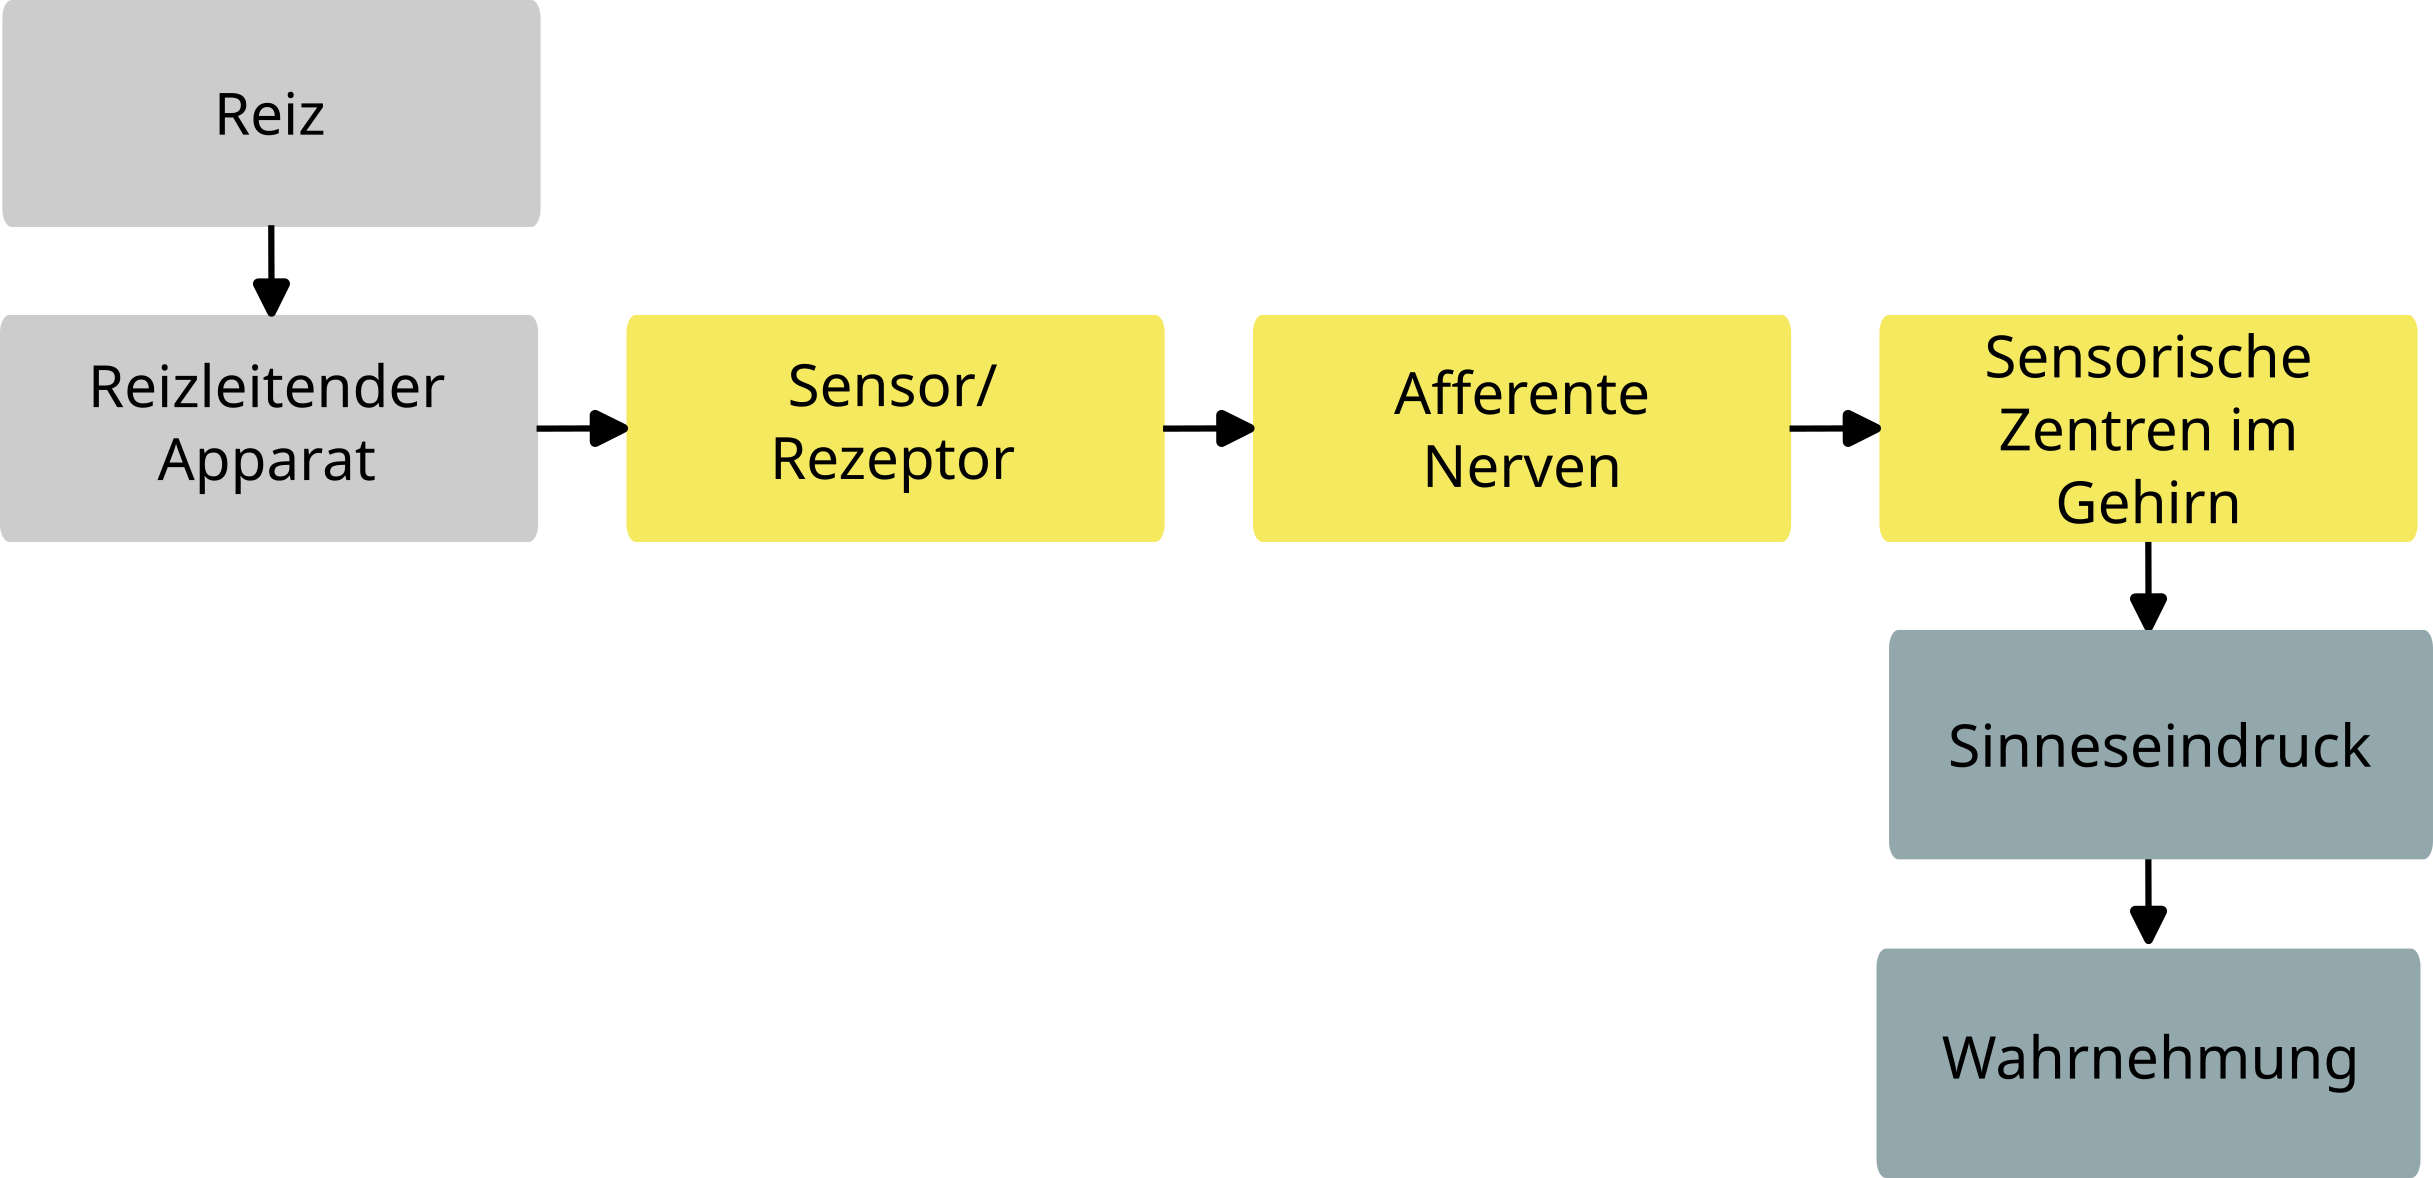
\includegraphics[width=\textwidth]{wahrnehmungsprozess_ohne_beispiel_ab_sensor.png}
\end{center}



\end{frame}


%  % Learning Objectives
 
\begin{frame}

 \frametitle{Nach dieser Vorlesung sollten Sie folgendes können}



\begin{block}{Grundlagen:}




\begin{itemize}

    \item 
den Aufbau der Retina beschreiben
    \item 
die Rolle des Pigmentepithels erläutern
    \item 
die molekularen und zellulären Grundlagen der Photorezeption erläutern
    \item 
photopisches und skotopisches Sehen beschreiben und erklären
    \item 
die Physiologie des Farbsehens beschreiben
    \item 
die Anatomie der Sehbahn beschreiben
    \item 
die Rolle von kortikalen Regionen beim Sehen beschreiben
    \item 
die Rolle efferenter Verbindungen beim Sehen erläutern
    \item 
die Grundlagen des Tiefensehens erklären
\end{itemize}


\end{block}

\end{frame}

\begin{frame}

 \frametitle{Nach dieser Vorlesung sollten Sie folgendes können}

 

\begin{block}{Klinik:}

\begin{itemize}
    
\item 
Anomalien im Farbsehen benennen und erklären
    \item 
Perimetrie beschreiben und Anwendungen erklären
    \item 
Ausfälle des Gesichtsfeldes erklären und beschreiben
    \item 
Diplopie definieren und erklären
    \item 
Strabismus definieren und erklären

\end{itemize}


\end{block}



\end{frame}



%% %% %% Main Body


%%%%%%%%%%%%%%%%%%%%%%%%%%%%%%%%%%%%%%%%%
%% Wahrnehmungsbahn: Sensor/Rezeptor
%%%%%%%%%%%%%%%%%%%%%%%%%%%%%%%%%%%%%%%%%

%% Wahrnehmungsbahn: Sensor
\begin{frame}{Photorezeption}
    \begin{center}
        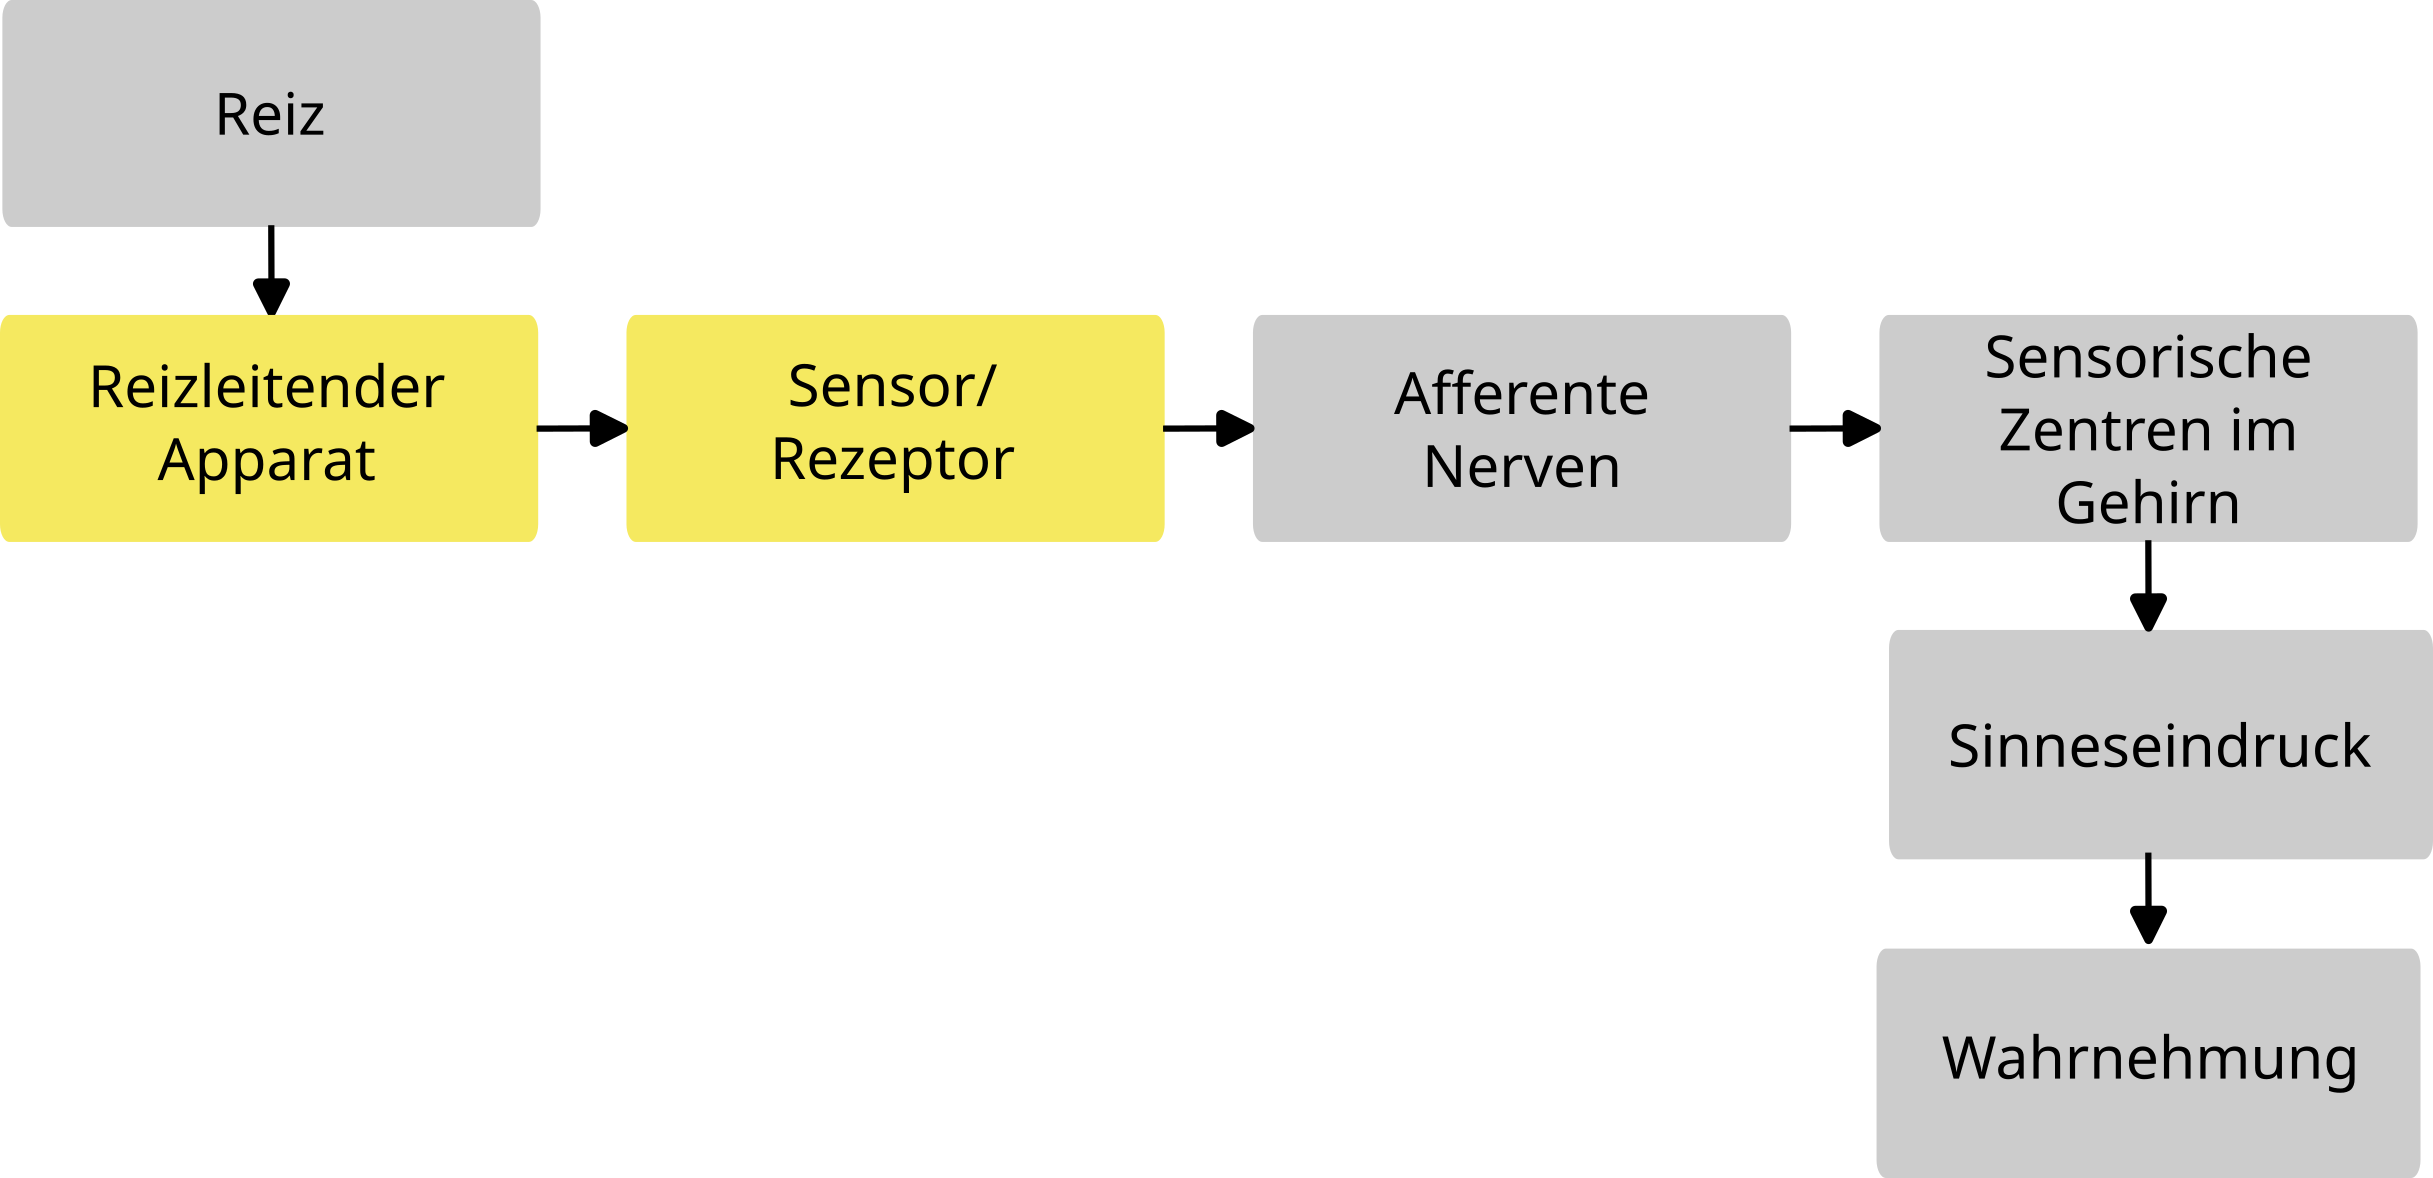
\includegraphics[width=\textwidth]{wahrnehmungsprozess_ohne_beispiel_apparat_und_sensor.png}
        
    \end{center}
\end{frame}


%% Aufbau der Retina 3-11

    %% Retina foto, fovea
\begin{frame}{Retina}
    

    \begin{columns}[c]
    
    \begin{column}{5cm}
    \begin{center}
        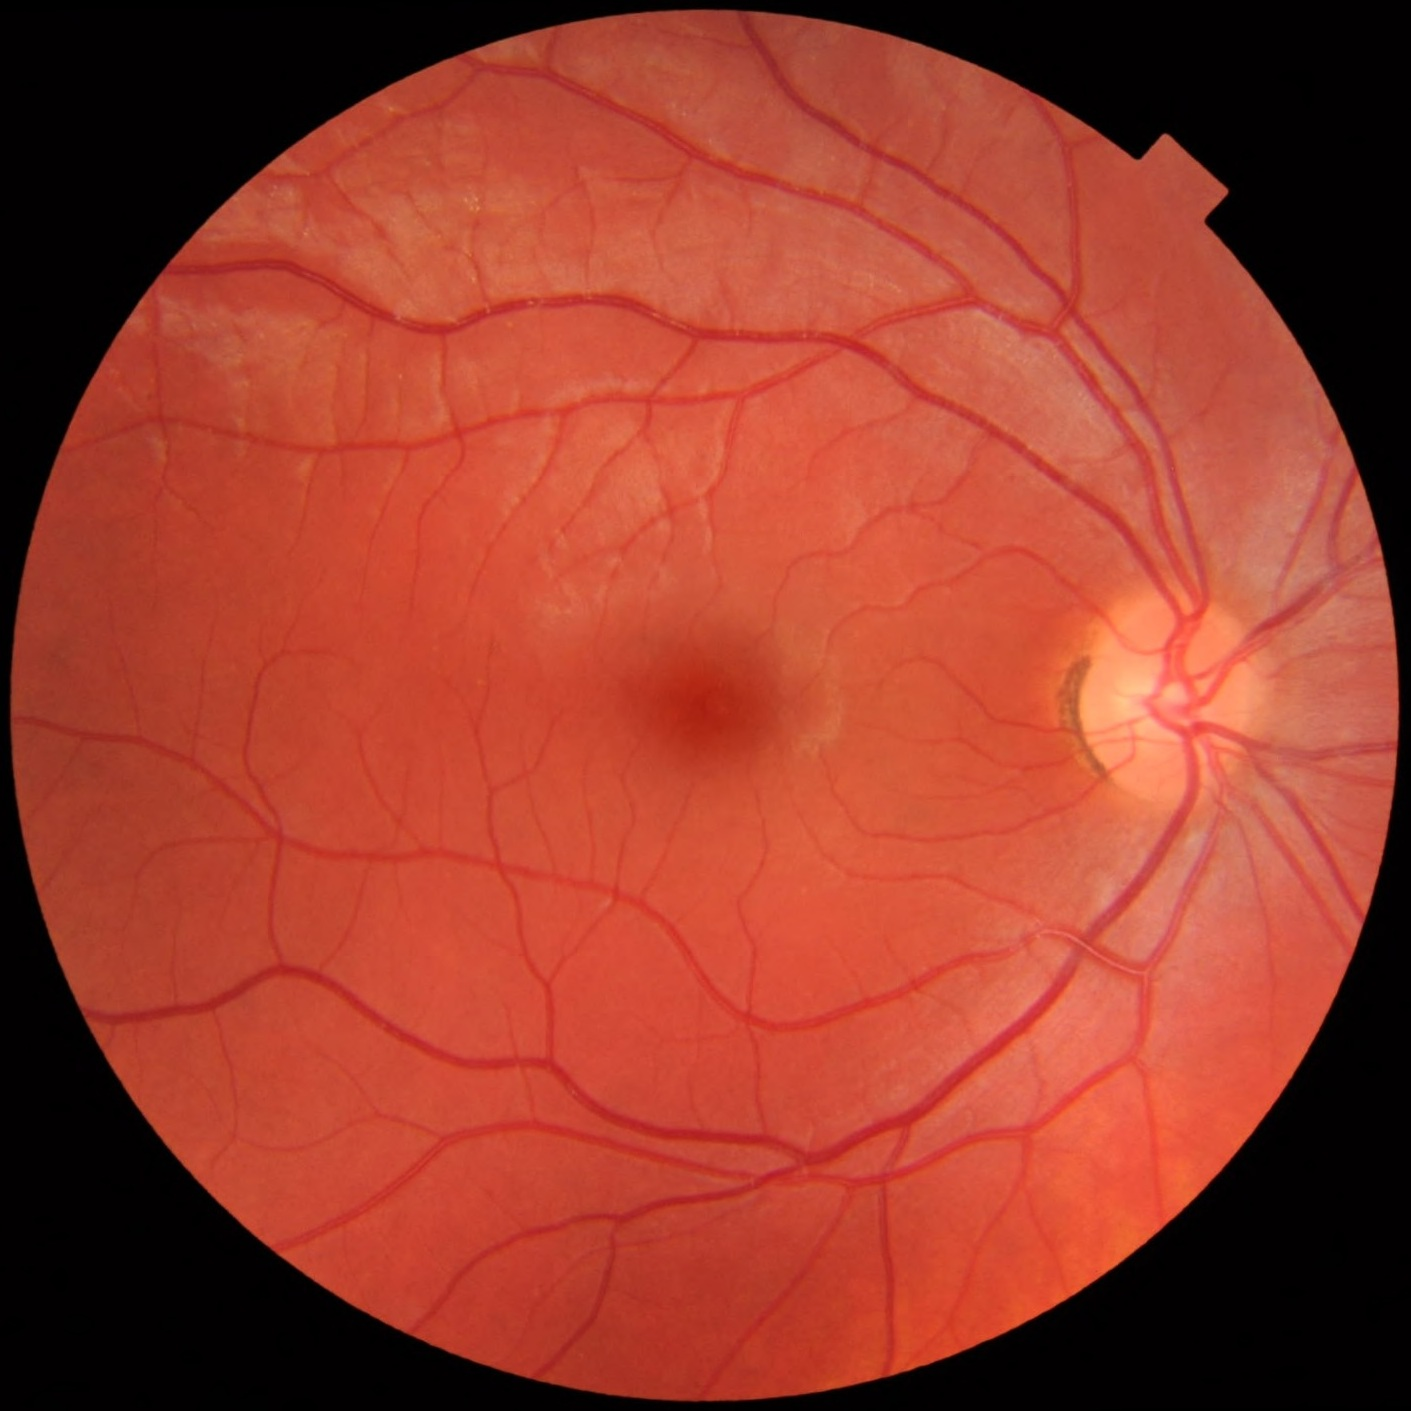
\includegraphics[width=\textwidth]{Fundus_photograph_of_normal_right_eye.jpg}
    \end{center}
    
    \end{column}


    \begin{column}{5cm}
Zu erkennen sind \pause \\
\begin{itemize}
    \item 
    Blutgefäße 
    \item
    Papilla (Ort des Durchtritts von Gefäßen und Nervus Opticus, nasal, hier rechts)
    \item
    Macula lutea (gefäßfreie Zone, Mitte)
\end{itemize}
    \end{column}
    
    \end{columns}

\end{frame}    
    

    % Fovea
    
\begin{frame}{Die Fovea ist der Ort der größten Sehschärfe}



\begin{columns}[c]
    
    \begin{column}{4cm}
    
        Der gelbe Fleck (Macula lutea) ist deshalb gelb, weil eingelagerte Carotinoide UV-Licht absorbieren, um Zellen davor zu schützen.  \\
        
        Innerhalb der Macula ist die Fovea Centralis, der Ort der größten Sehschärfe

    
    \end{column}


    \begin{column}{7cm}

    \begin{center}
        \includegraphics[width=\textwidth]{Macula.png}
    \end{center}

    \end{column}
    
    \end{columns}
    
\end{frame}


    
    
    
    %% Zelltypen der retina
    \begin{frame}{Zelltypen in der Retina}
    
    \begin{center}
        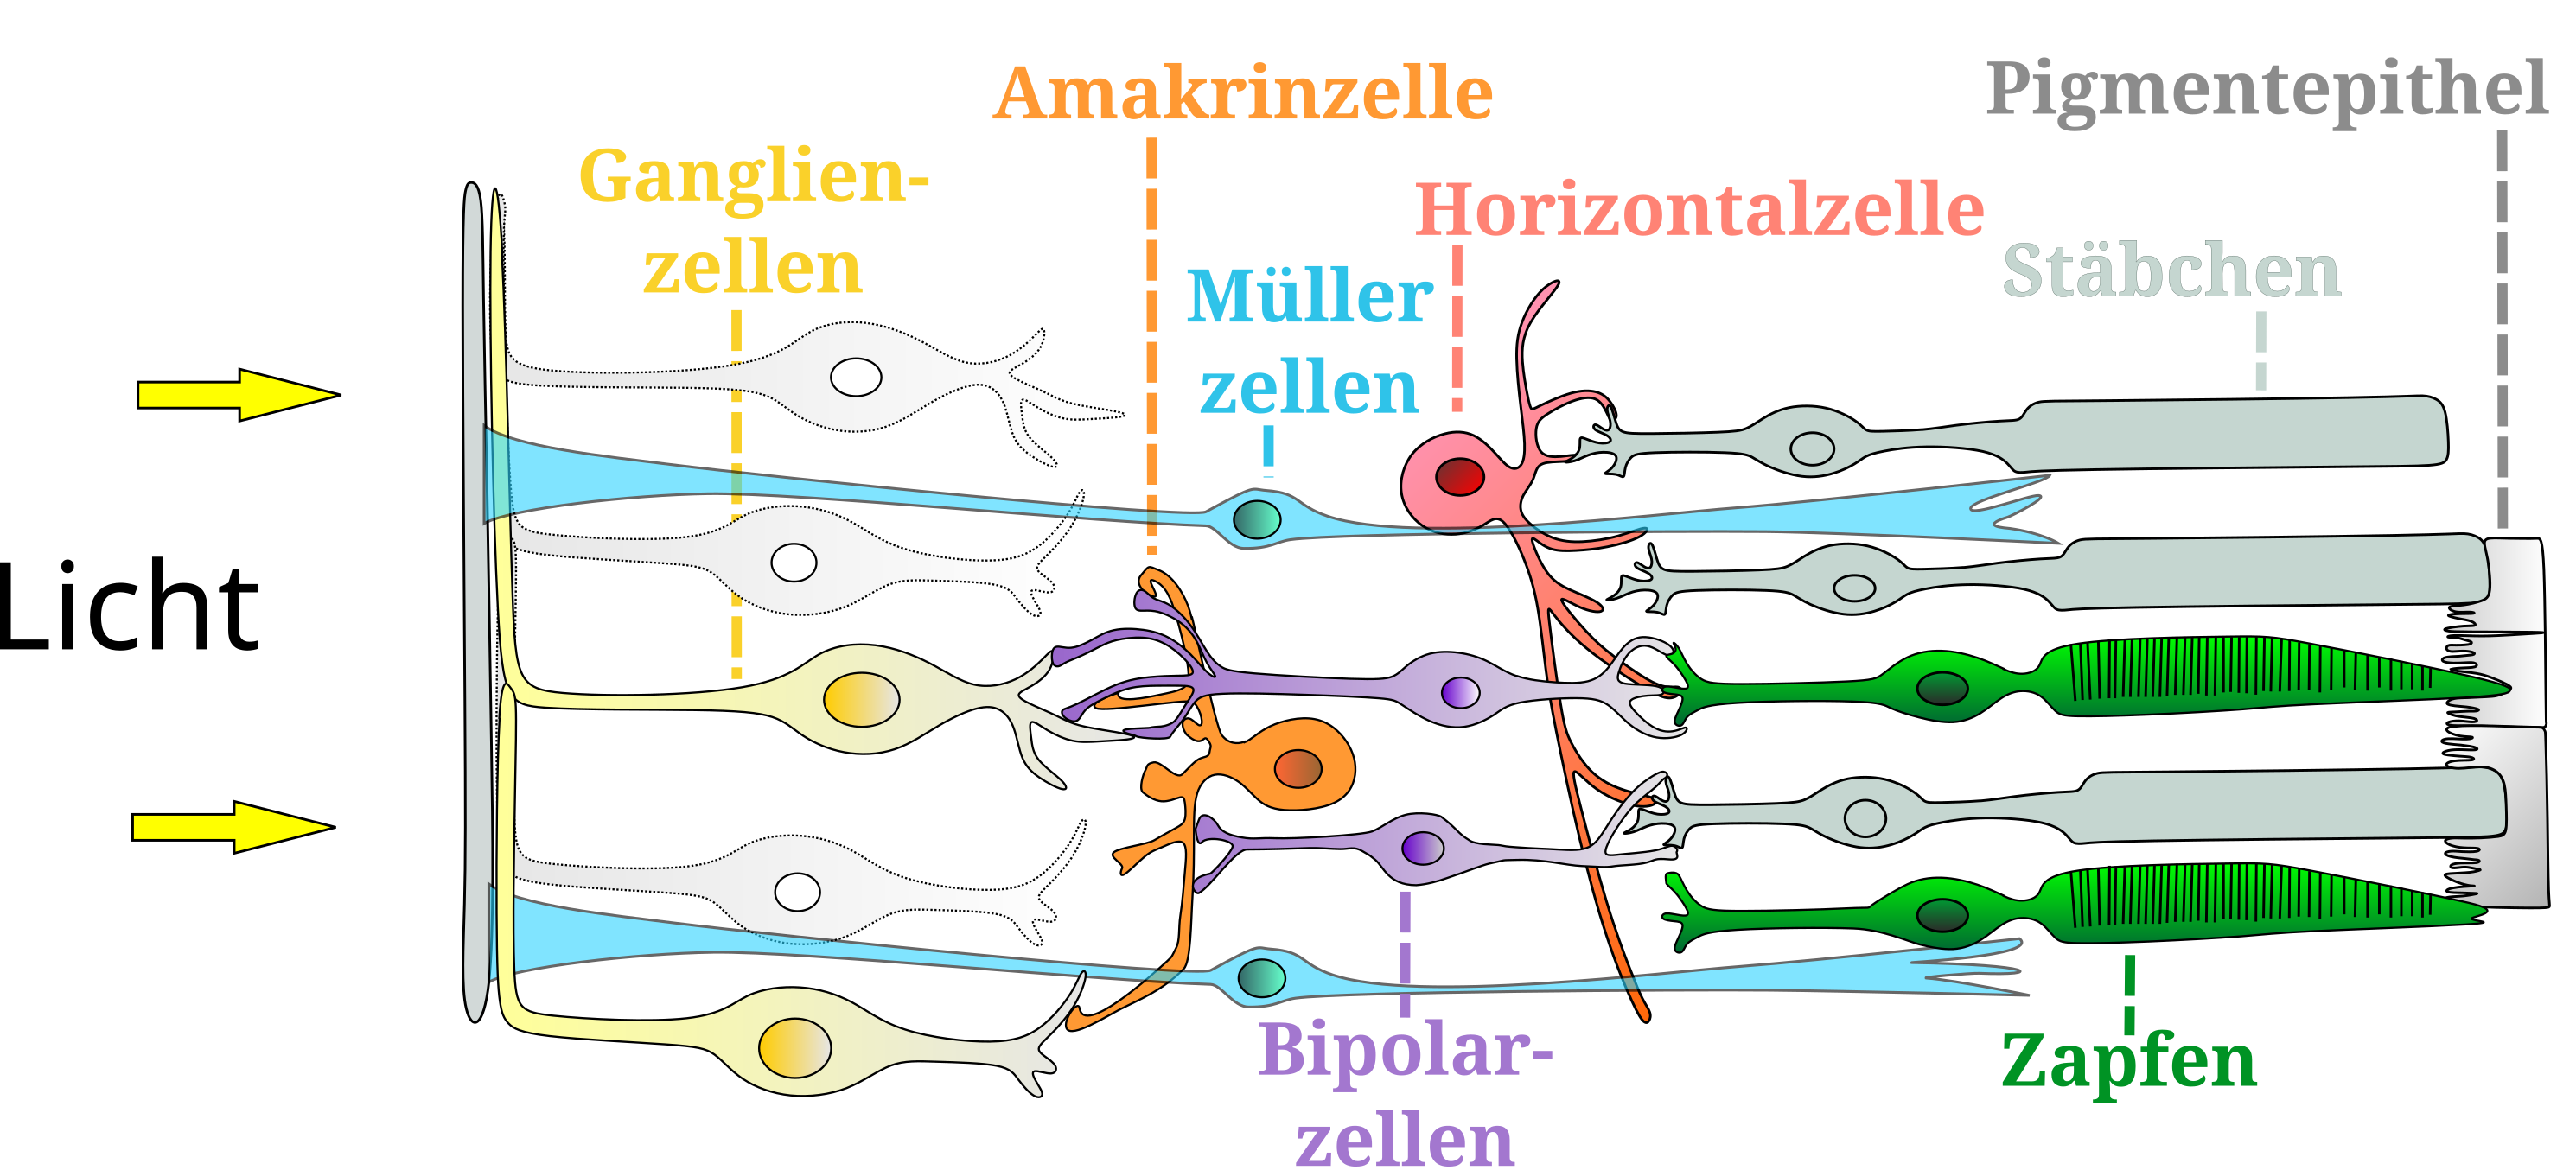
\includegraphics[width=\textwidth]{Retina_de.png}
    \end{center}
        
    \end{frame}
    
    
    %% Gegenüberstellung Stäbchen, Zapfen
    
    \begin{frame}{Choose your fighter: Stäbchen vs Zapfen}


\begin{columns}[c]

\begin{column}{2.5cm}
\textbf{Stäbchen:} \\[0.5 cm]

1 Typ \\

Ca. 110 Millionen  \\

Geringe räumliche Auflösung (Verschaltung mit Ganglienzellen bis zu 3000:1) \\

Sehr lichtsensitiv \\
\end{column}


\begin{column} {6 cm}
    \begin{center}
        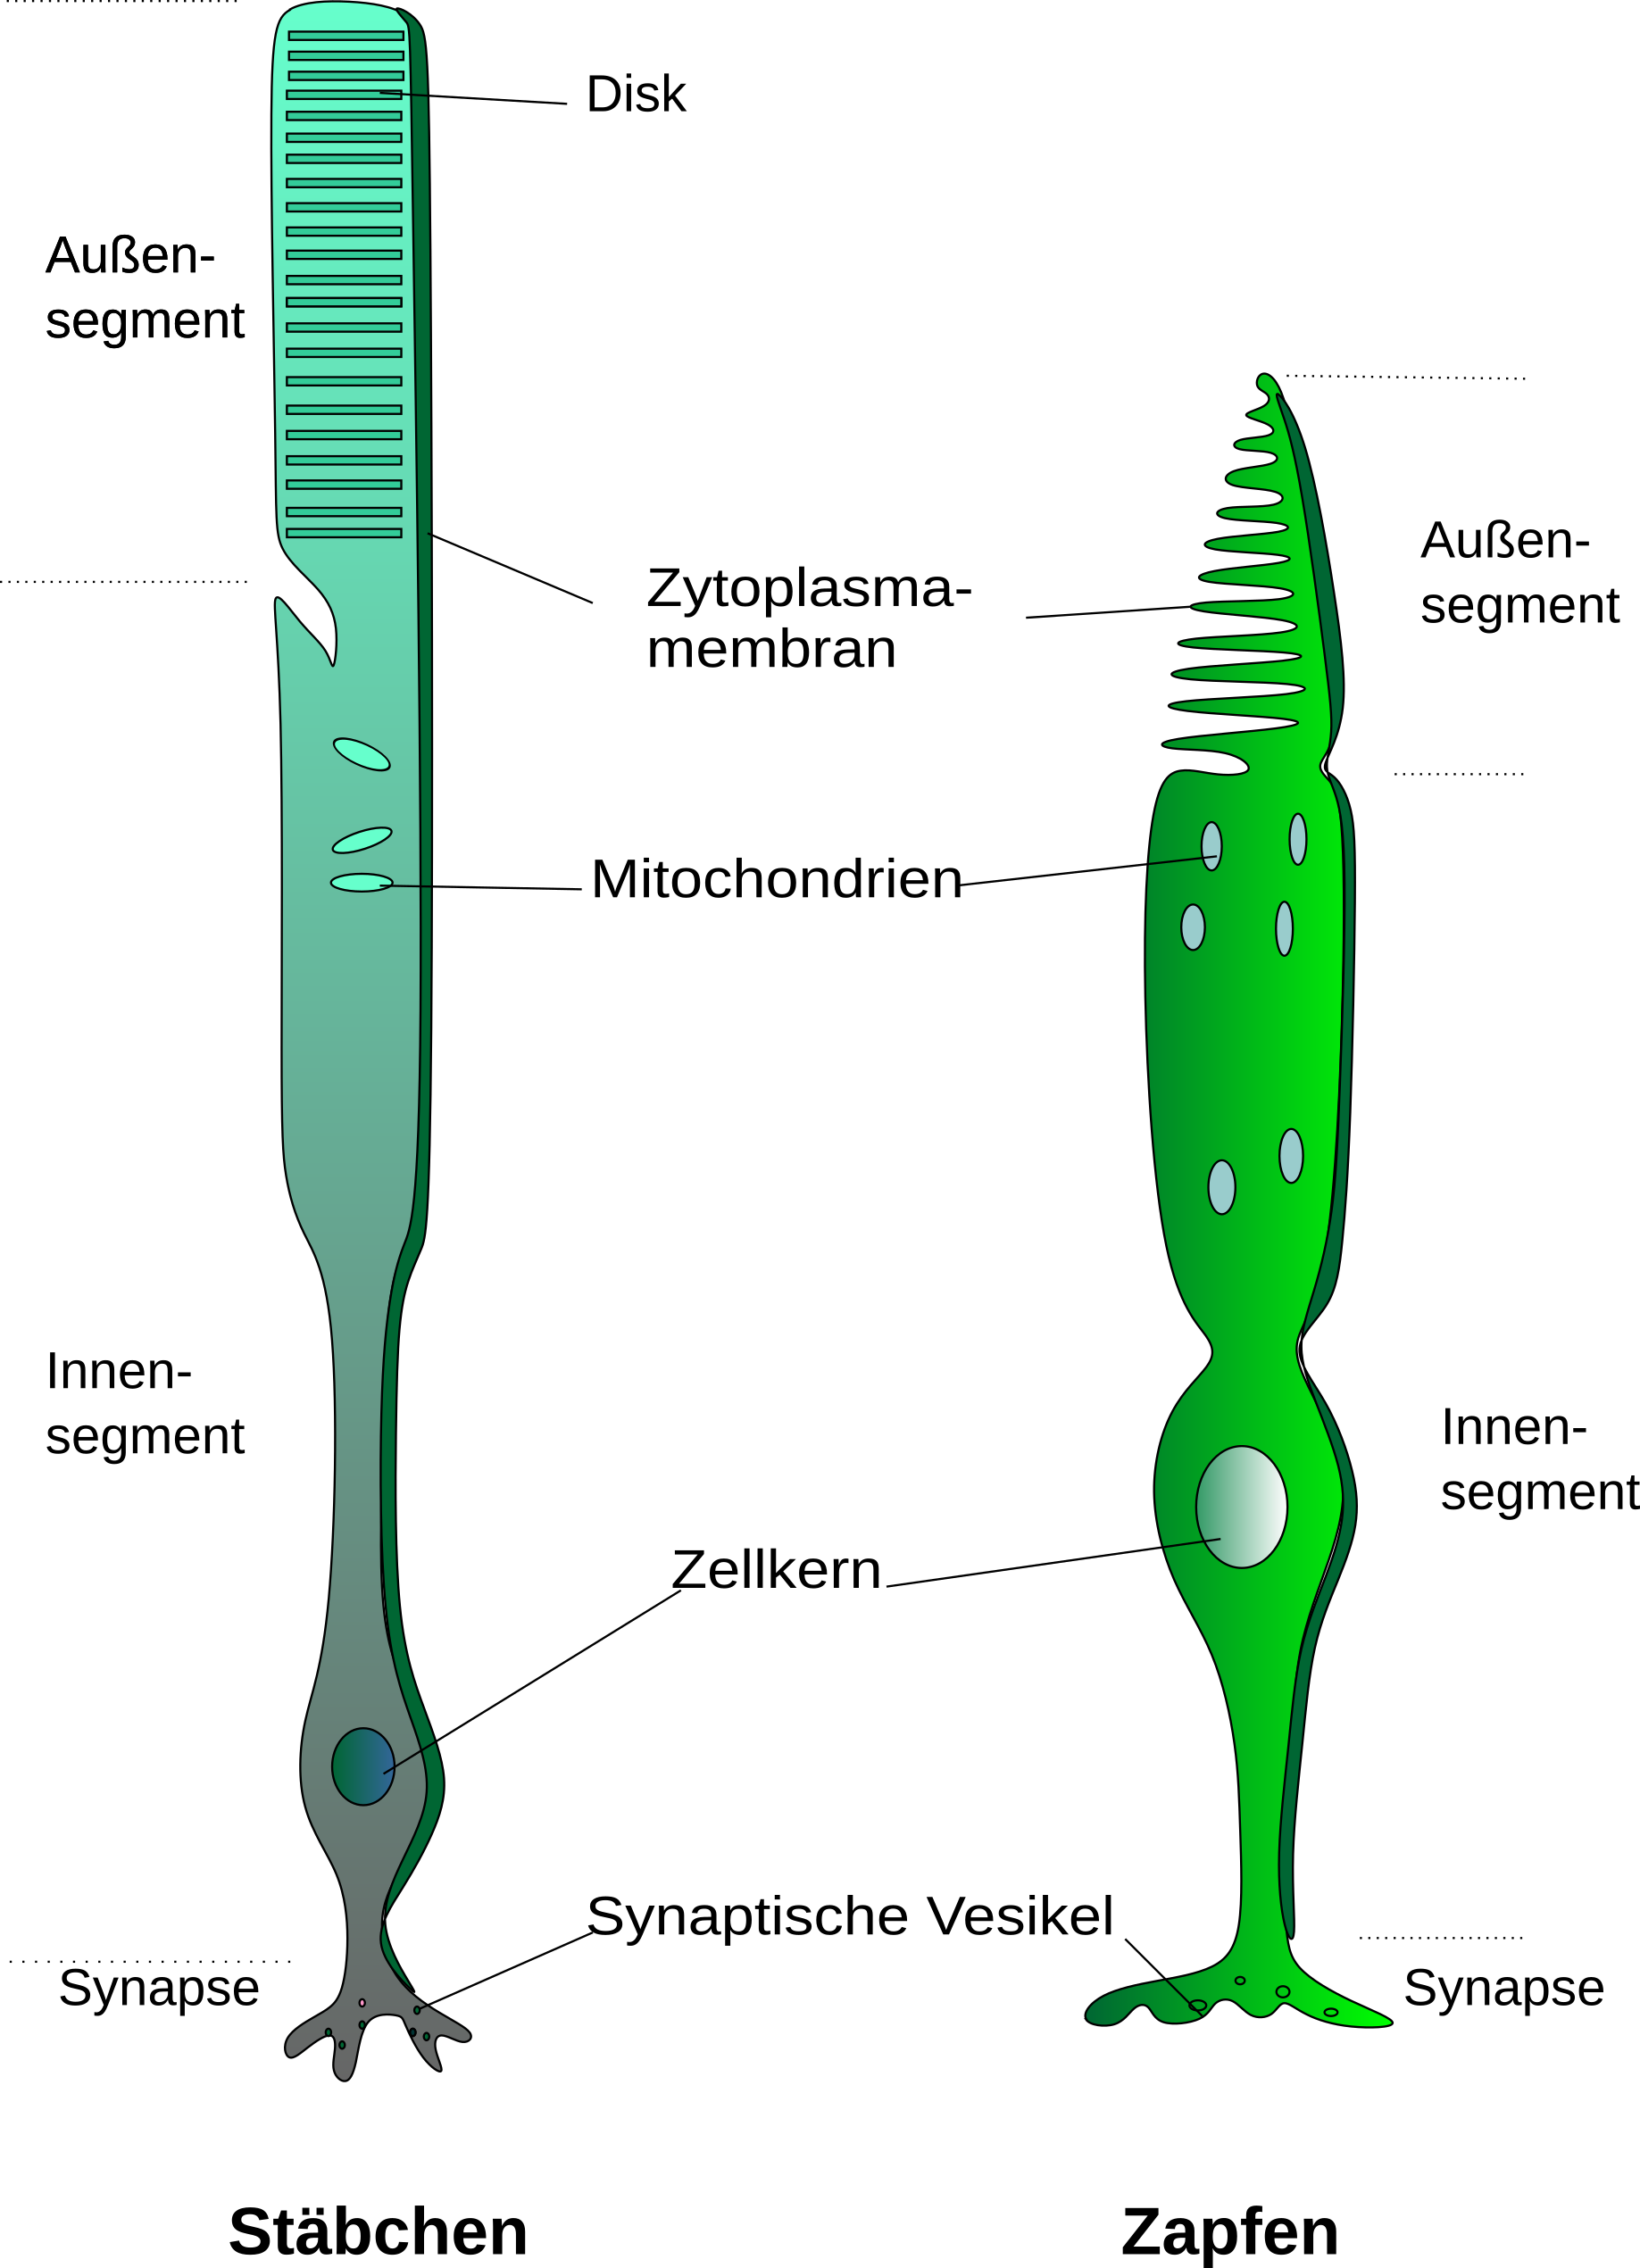
\includegraphics[width=1\textwidth]{Cone_rode.png}
    \end{center}

\end{column}



\begin{column}{2.5cm}

\textbf{Zapfen:} \\[0.5 cm]

3 Typen \\

Ca. 6 Millionen   \\

Hohe räumliche Auflösung (in Foveola 1:1 mit Ganglienzellen)  \\

Verantwortlich für Farbensehen \\
\end{column}


\end{columns}    
        
    \end{frame}
    
    

    %% Verteilung von staäbchen und zapfen

    
    
    \begin{frame}{Stäbchen und Zapfen sind unterschiedlich verteilt}

    \begin{center}
        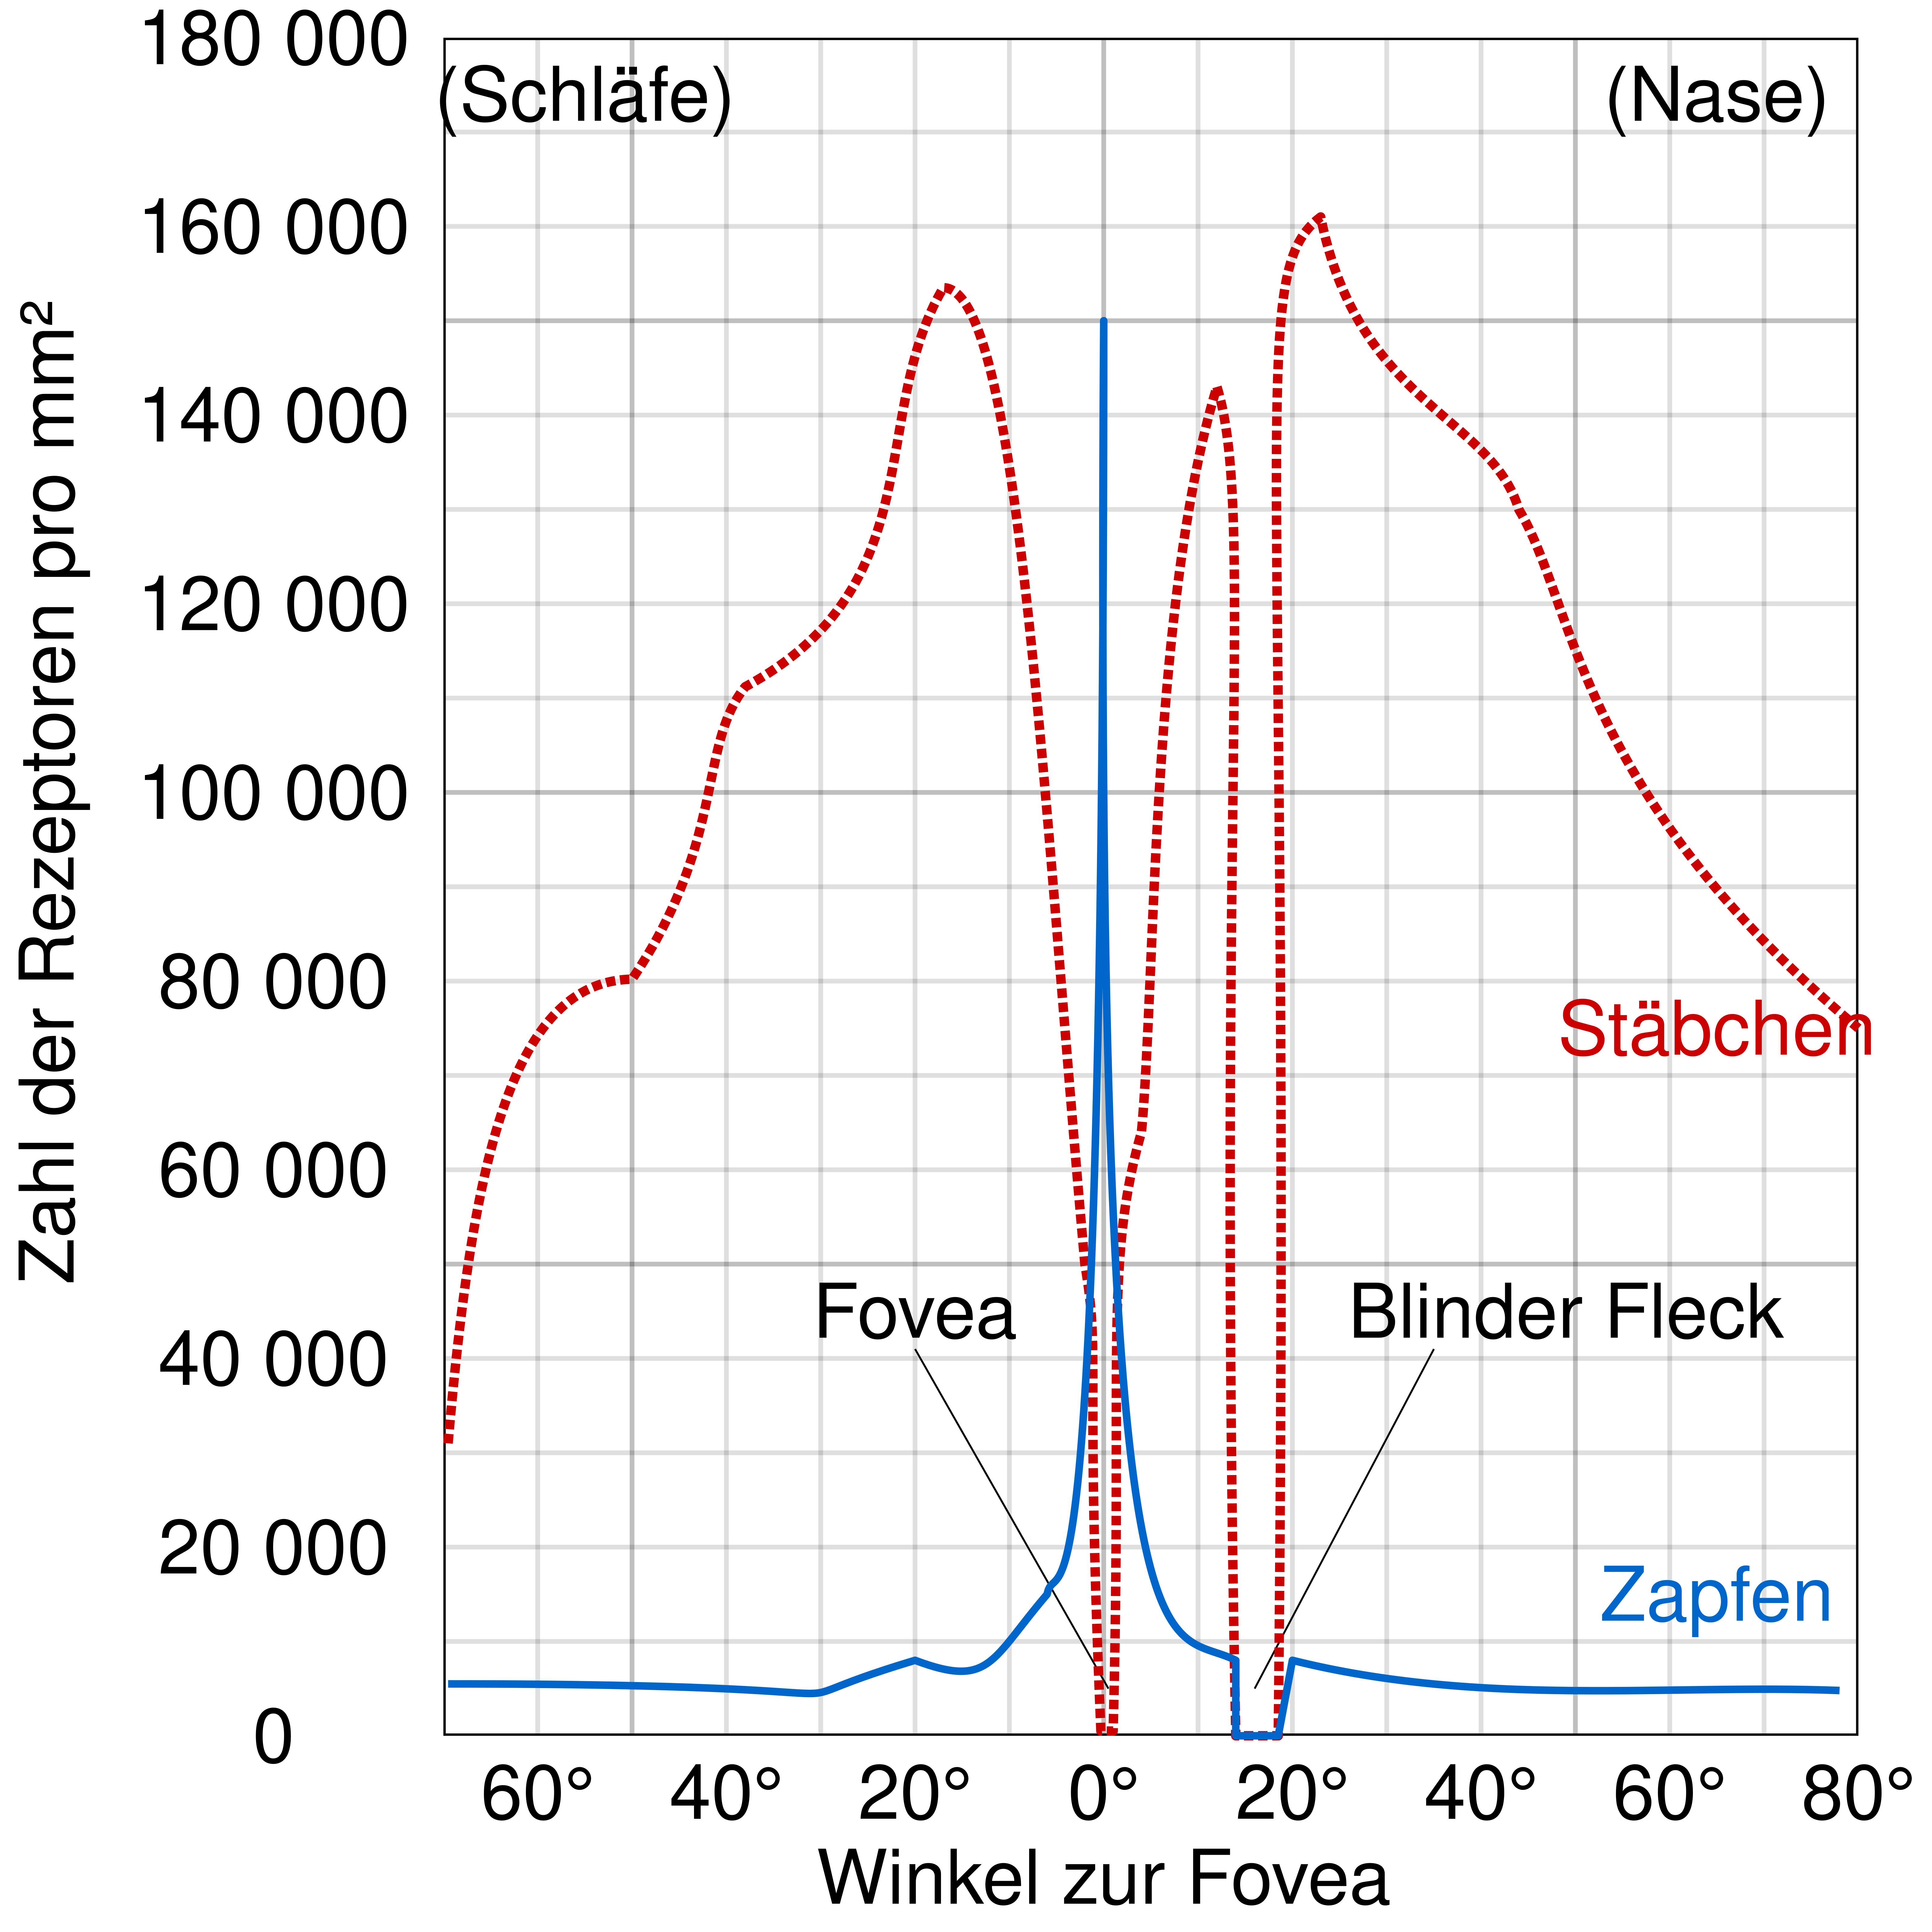
\includegraphics[width=0.6\textwidth]{Human_photoreceptor_distribution.png}
    \end{center}



\end{frame}
    
    

%% Phototransduktion 12-23

\begin{frame}{Phototransduktion}

Photorezeptor-Zellen (Stäbchen und Zapfen) sind bei Dunkelheit depolarisiert (über stets aktive cGMP-gesteuerte Kationenkanäle): Dunkelstrom \\[0.5cm]


\pause
\begin{columns}[c]

\begin{column}{5cm}
Bei Lichteinwirkung: 11-cis-Retinal (Teil des Rhodopsin-Komplexes) wird umgewandelt in all-trans-Retinal. Dadurch wird das Rhodopsin aktiviert.

\end{column}

\begin{column}{6cm}
\begin{center}
    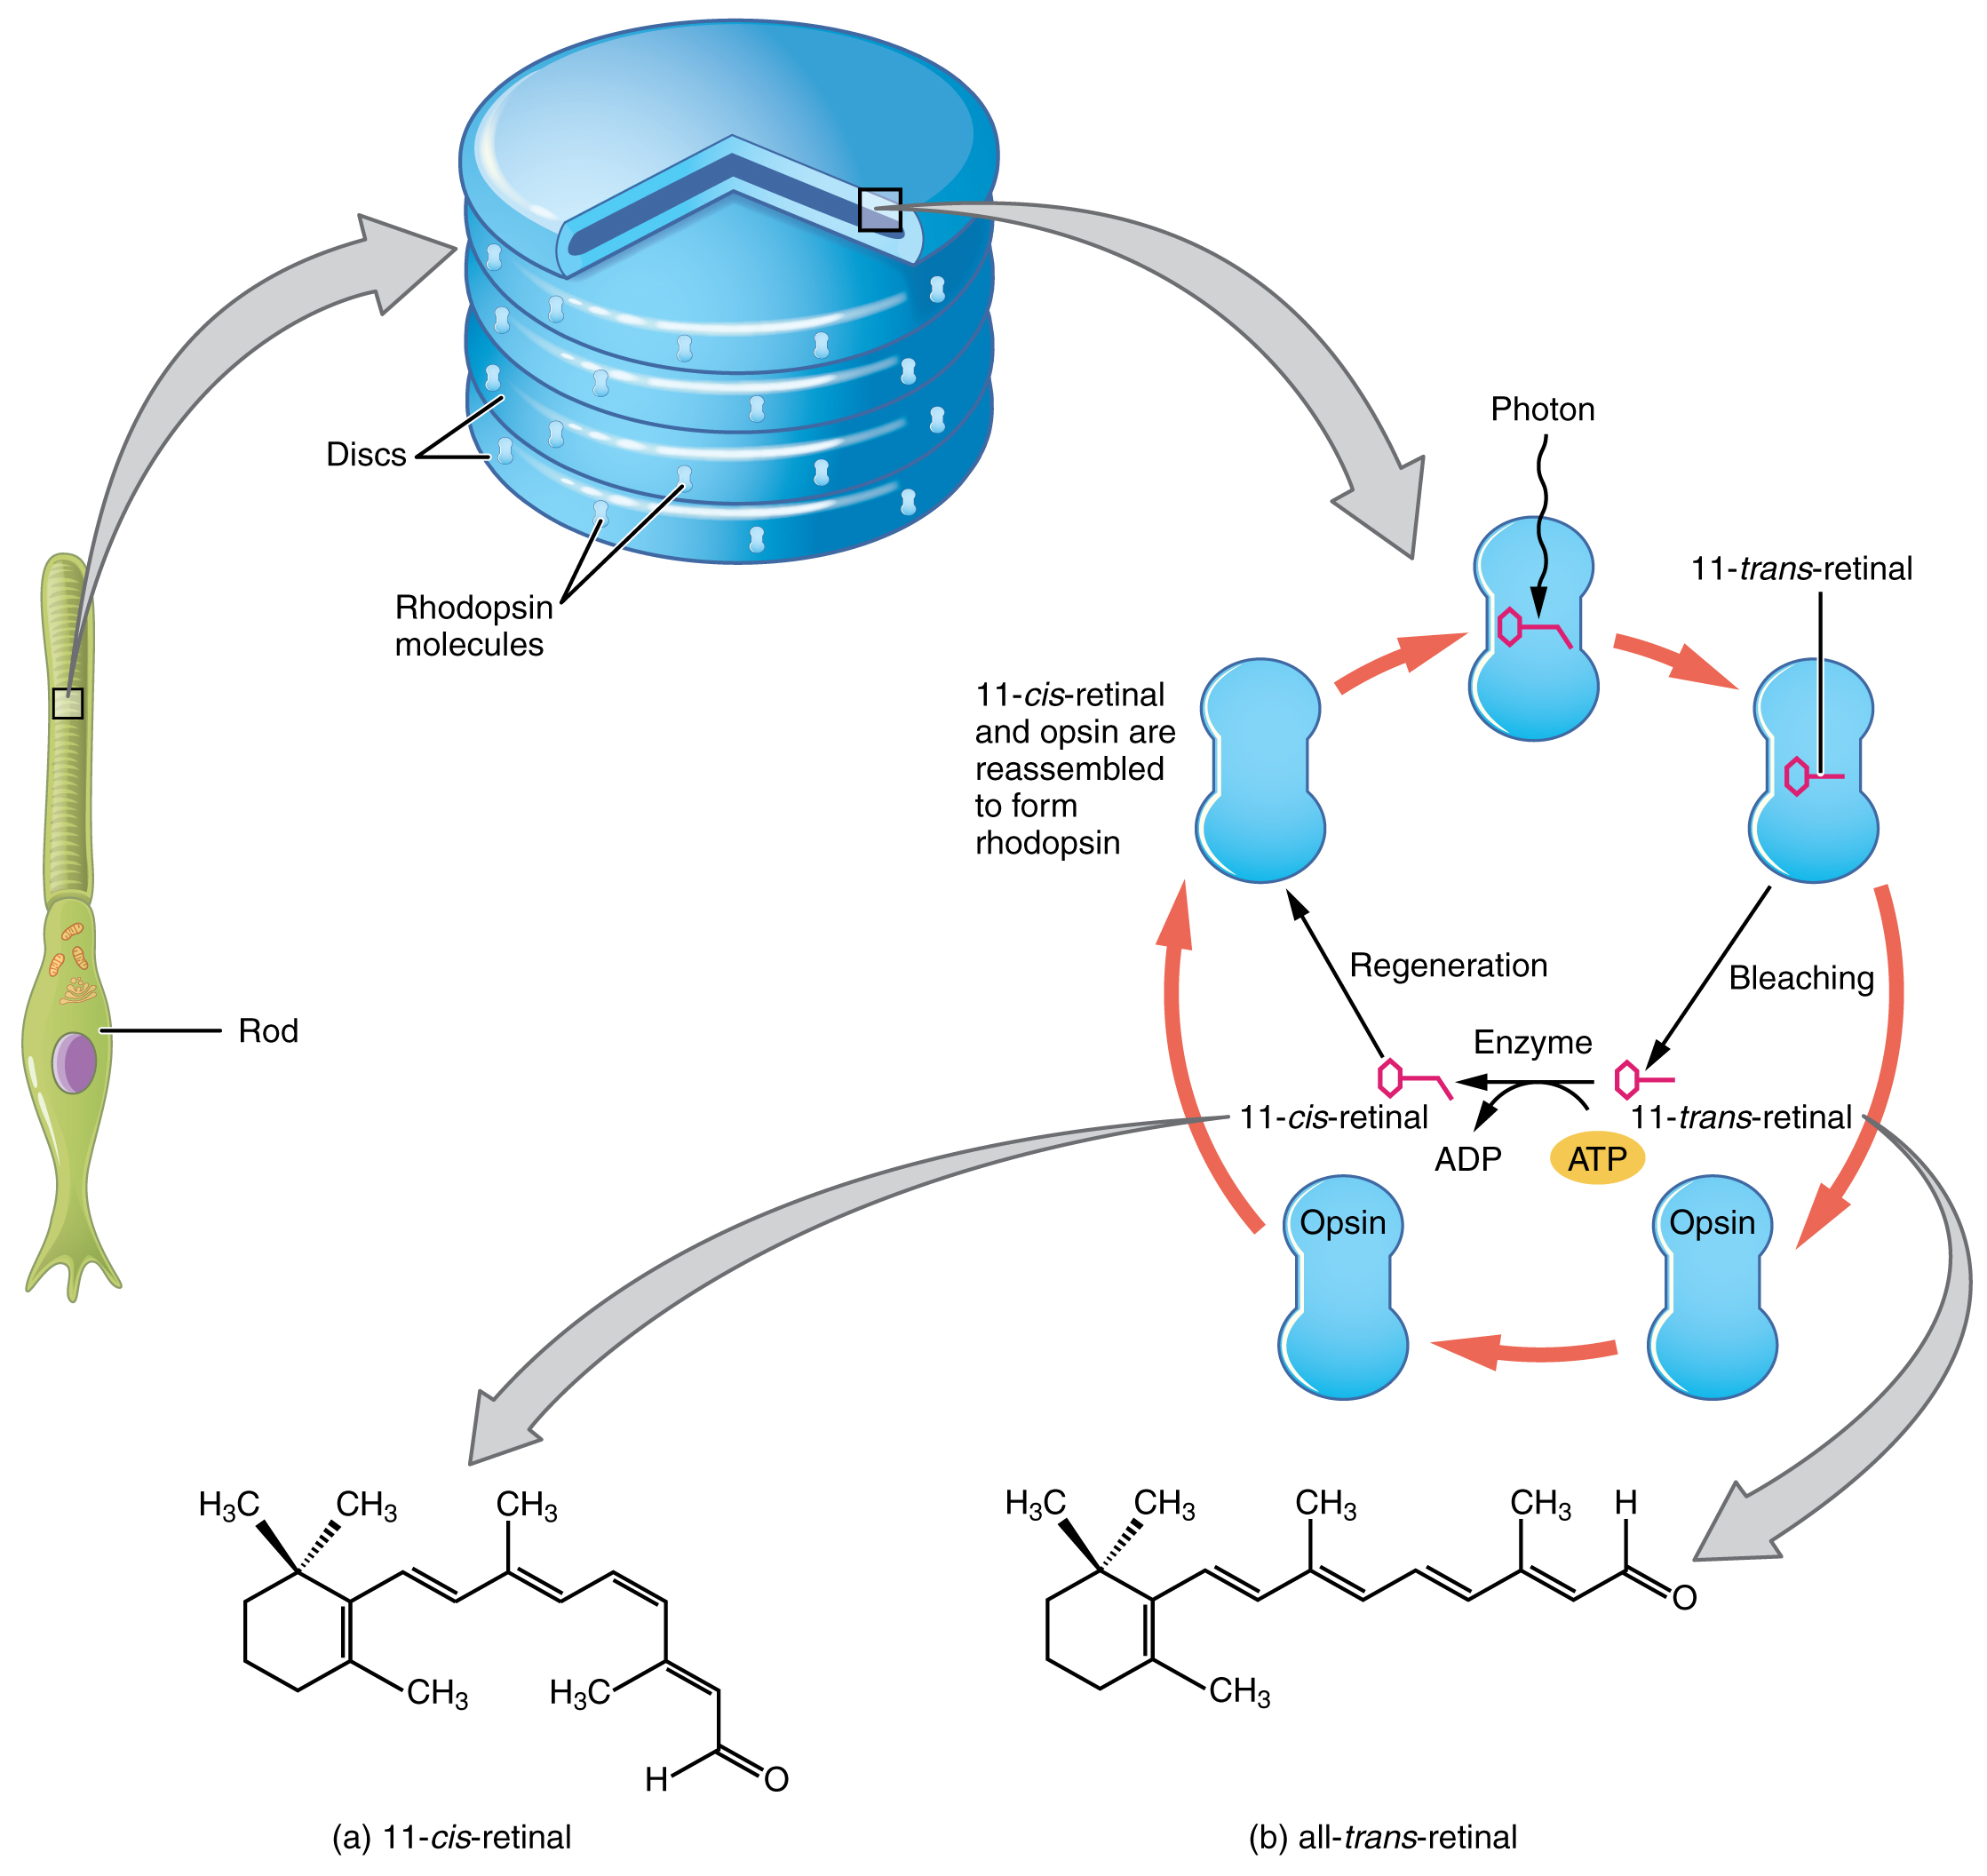
\includegraphics[width=\textwidth]{1415_Retinal_Isomers.jpg}
\end{center}

\end{column}


\end{columns}



    
\end{frame}

\begin{frame}{Phototransduktion}

Aktivierungskaskade: Aktiviertes Rhodopsin \(\rightarrow\) Transducin (G-Protein) \(\rightarrow\) Phosphodiesterase \(\rightarrow\) Hydrolysierung von cGMP zu 5'GMP.  \\[0.5 cm]

Aber was hat cGMP gemacht? \pause cGMP aktiviert die cGMP-gesteuerten Ionenkanäle (Dunkelstrom). Ohne cGMP werden diese Kanäle geschlossen, es kommt zu einer Hyperpolarisation der Membran (Inaktivierung der Zelle)

\begin{center}
    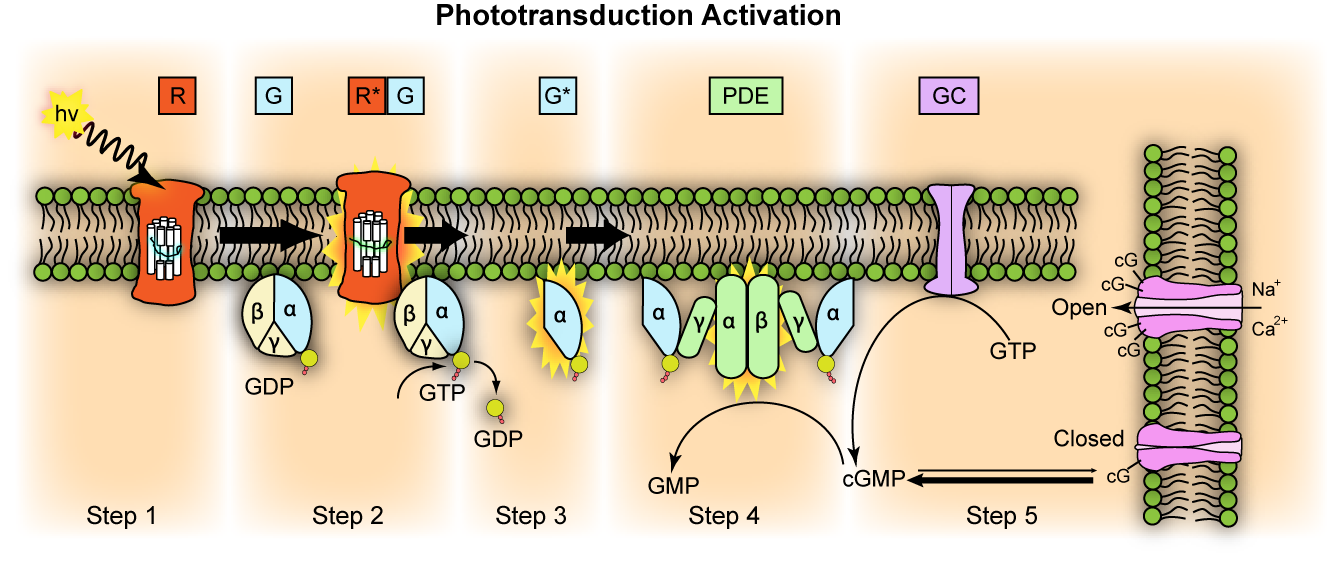
\includegraphics[width=\textwidth]{Phototransduction.png}
\end{center}
      
\end{frame}


\begin{frame}{"Recycling"}


\begin{itemize}
    \item 
    Die an der Phototransduktion beteiligten Moleküle müssen wieder in ihren Ausgangszustand zurückgeführt werden können, damit eine neue Signalkaskade beginnen kann. 
\item
Dies passiert zum Teil (Umwandlung von all-trans-Retinal in 11-cis-Retinal) im Pigmentepithel. 
\item
Aktiviertes Rhodopsin wird durch die Wirkung von R*-Kinase inaktiviert. Dieser Vorgang wird bei hohen Calcium-Konzentrationen gehemmt. 
\item
Durch Verzögern oder Verschnellern des Recycling-Prozesses kann kontrolliert werden, wie viele Moleküle für die Phototransduktion zur Verfügung stehen und daher, wie schnell die Phototransduktion läuft. 

\end{itemize}





    
\end{frame}


\begin{frame}{Wie geht es weiter?}

\begin{center}
    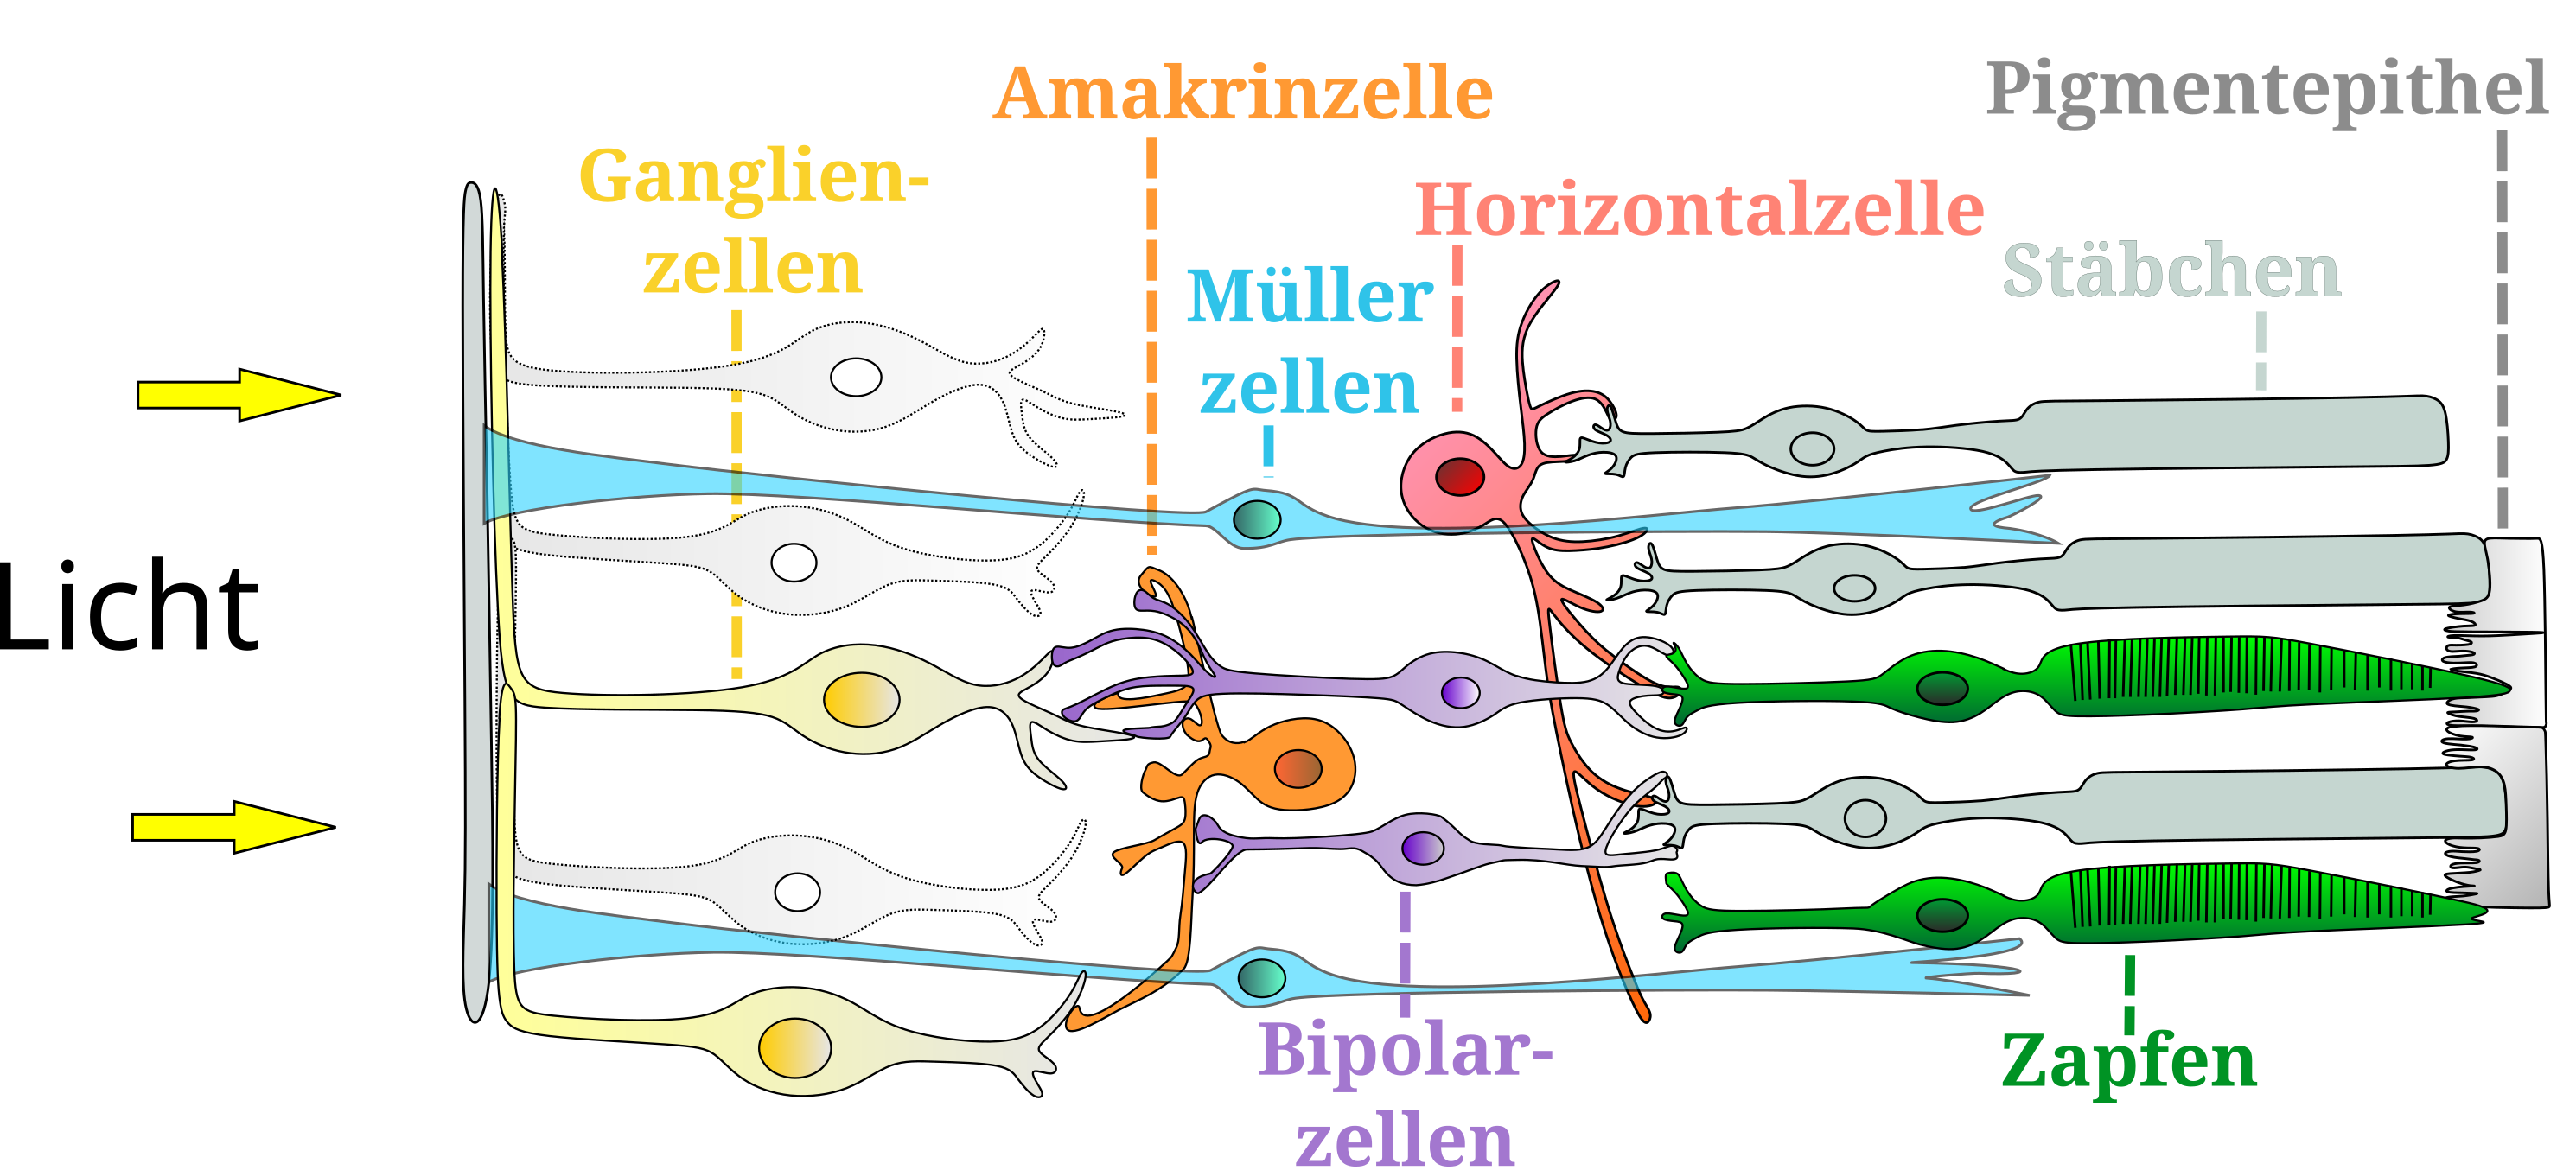
\includegraphics[width=\textwidth]{Retina_de.png}
\end{center}

\end{frame}


%% Retinale Signalverarbeitung: Bipoalarzellen 28-49

\begin{frame}{Zapfen leiten Signale an Bipolarzellen weiter}

Zwei Arten von Zapfen-Bipolarzellen: 

\begin{itemize}
    \item 
    Off-Bipolarzellen sind bei Dunkelheit aktiv (Verhalten sich wie Zapfen)
    \item
    On-Bipolarzellen sind bei Licht aktiv (Verhalten sich gegensätzlich)
\end{itemize}

\pause

Zapfen aktivieren Off-Bipolarzellen durch Ausschüttung von Glutamat und hemmen On-Bipolarzellen \emph{wie}?

\pause

Erstaunlicherweise auch durch Glutamat! (Über einen metabotropen Glutamatrezeptor an der On-Zelle) \\[0.5 cm]


\pause
Warum brauchen wir einen On- und einen Off-Weg?

Höhere Sensitivität für Veränderungen der Helligkeit.  \\


\end{frame}



    
    
\begin{frame}{Bipolarzellen leiten an retinale Ganglienzellen weiter}

\begin{center}
    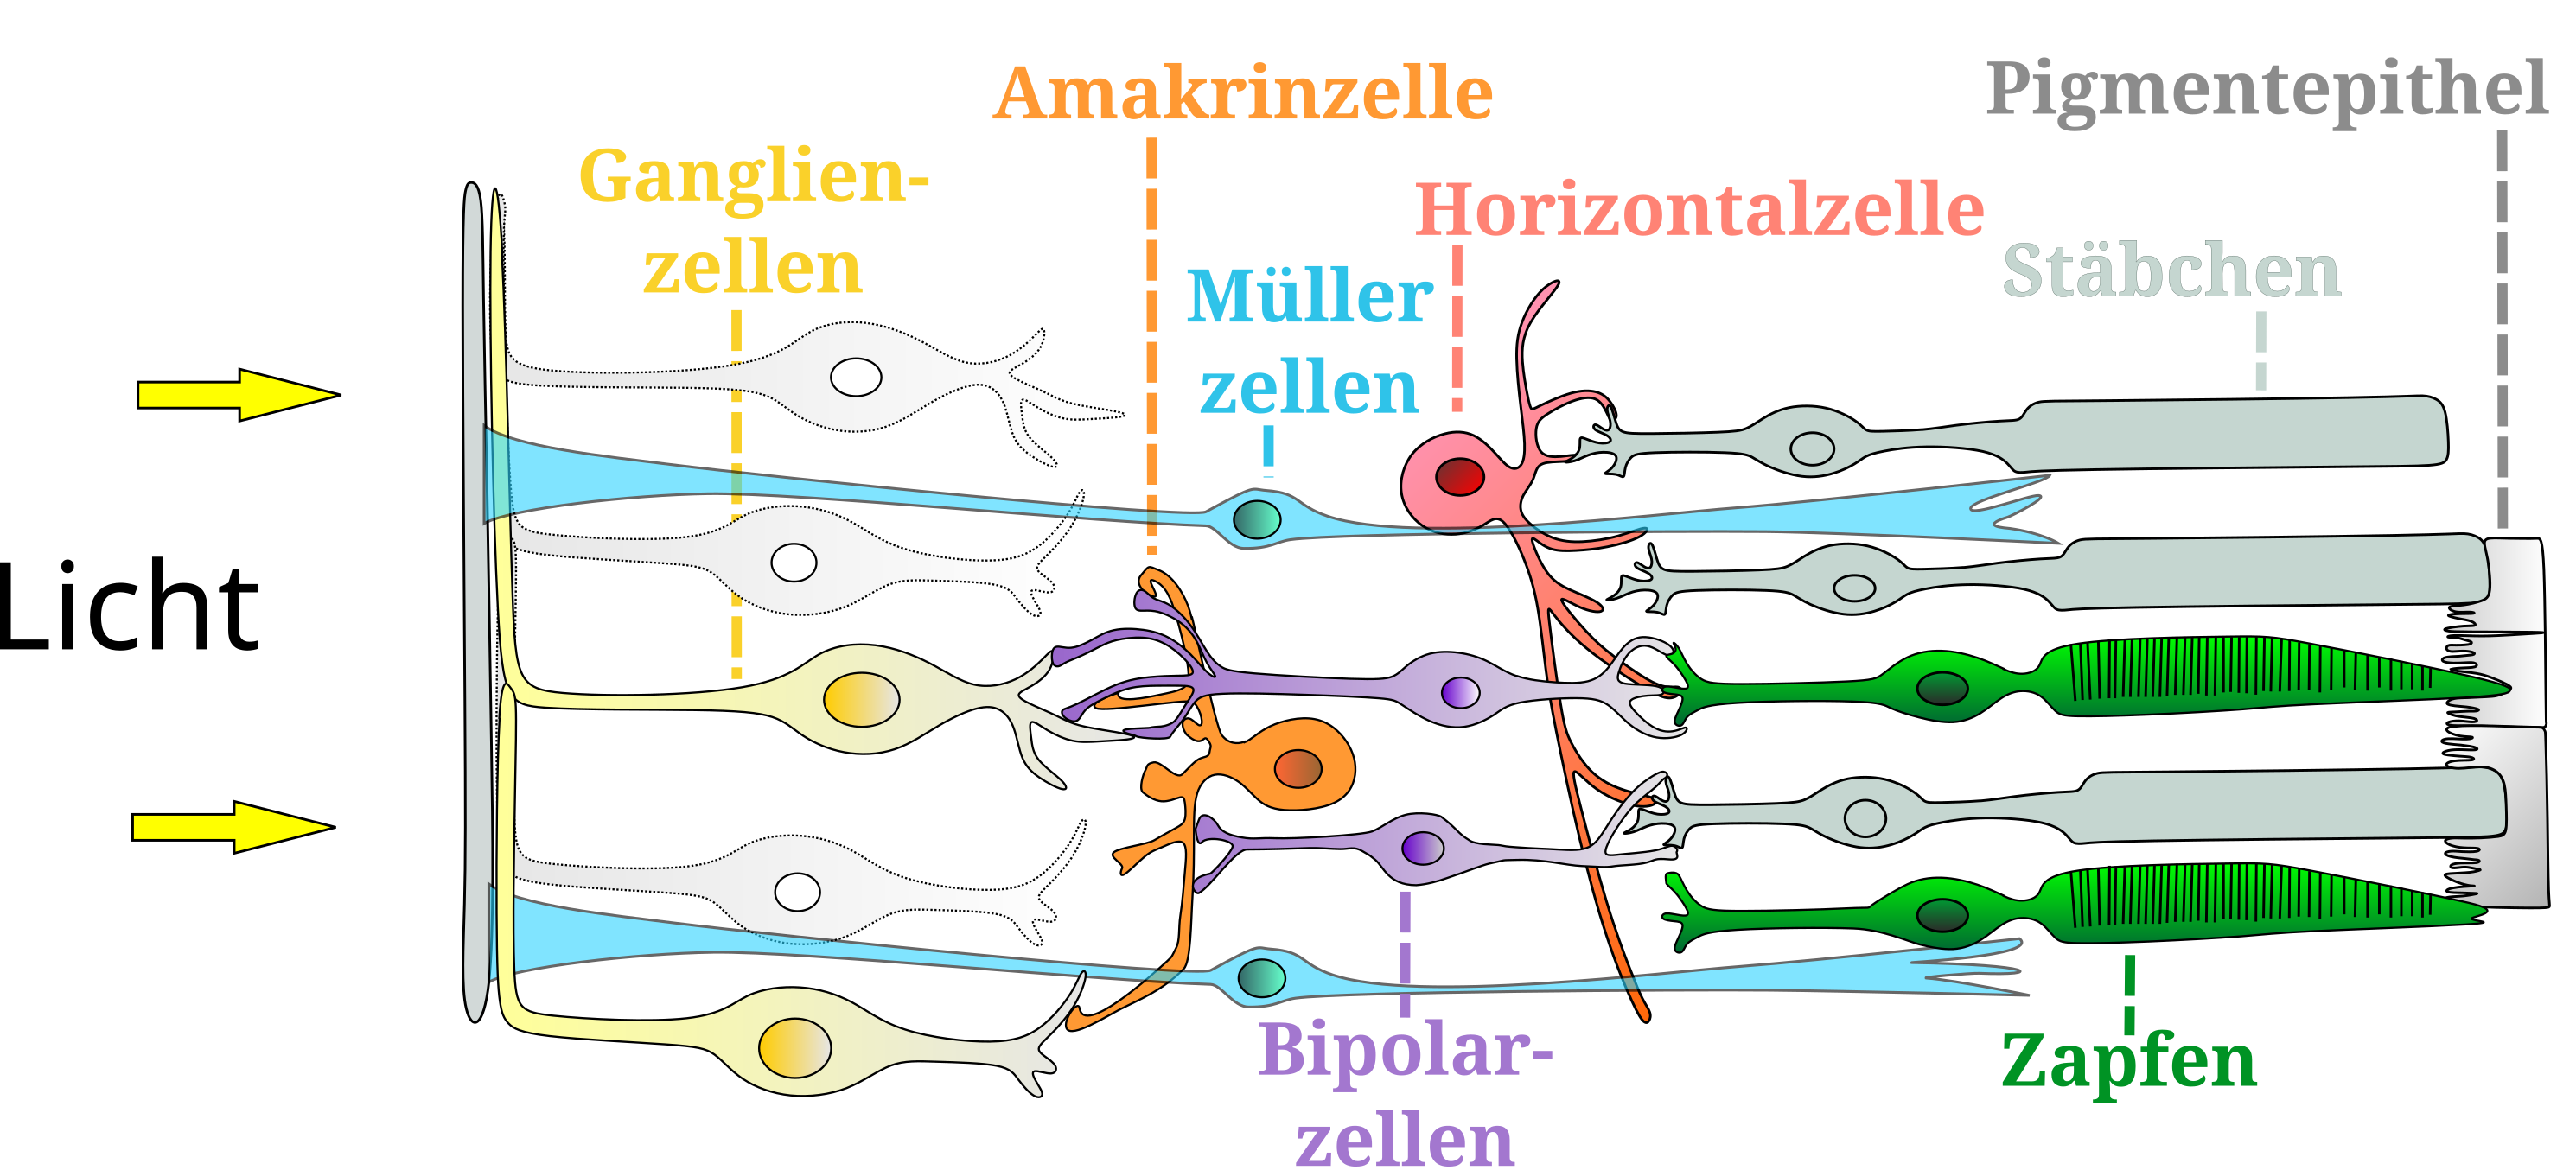
\includegraphics[width=\textwidth]{Retina_de.png}
\end{center}

    
\end{frame}




%% Retinale Ganglienzellen (Buch)
\begin{frame}{Das Aktionspotential wird in den Ganglienzellen erzeugt}

Es gibt On- und Off-Ganglienzellen, analog zu den On- und Off-Bipolarzellen

\begin{center}
    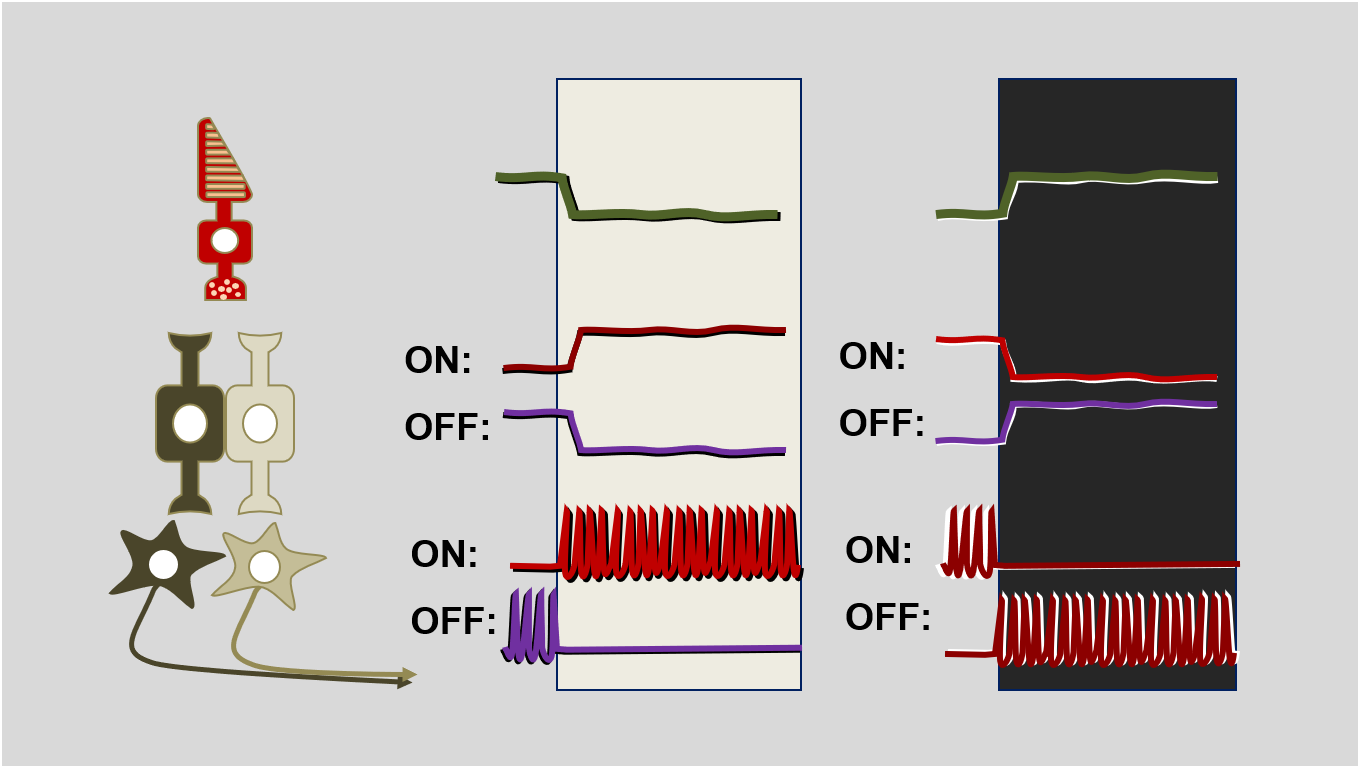
\includegraphics[width=\textwidth]{on_off_bipolarzellen.png}
\end{center}


\end{frame}


%% Klassifizierung retinaler Ganglienzellen 
\begin{frame}{Klassen retinaler Ganglienzellen}

\begin{itemize}
    \item 
    Magnozelluläre Ganglienzellen (10\,\%): Große Zellkörper, große rezeptive Felder, gute zeitliche Auflösung. Wahrnehmung von Bewegung und Kontrast.
    \pause
    \item
    Parvozelluläre Ganglienzellen: (80\,\%): Kleine rezeptive Felder, gute räumliche aber schlechte zeitliche Auflösung, farbempfindlich. Wahrnehmung von Farbe und Form.
    \pause
    \item
    "Sonstige" (10\,\%):
    \begin{itemize}
        \item Koniozelluläre Ganglienzellen: Blau-Gelb-Wahrnehmung
        \item Bewegungs-spezifische Ganglienzellen: Unbewusste Wahrnehmung von Bewegung
    \item Melanopsin-positive Ganglienzellen: Intrinsisch lichtempfindlich; Pupillenreflexe, Tag-Nacht-Rhythmus
    \end{itemize}
\end{itemize}


\end{frame}


%% IMPP Frage zu Ganglienzellen
\begin{frame}{IMPP Frage}

Welche der folgenden Aussagen zu retinalen Ganglienzellen trifft charakteristischerweise zu?

\begin{description}
\item[A.] Off-Ganglienzellen erhalten Signale direkt von Bipolarzellen, die über ionotrope Glutamatrezeptoren direkt von Zapfen depolarisiert werden. %% richtig
\item[B.] Off-Ganglienzellen erhalten Signale direkt von Bipolarzellen, die über metabotrope Glutamatrezeptoren direkt von Zapfen hyperpolarisiert werden. 
\item[C.] Off-Ganglienzellen erhalten Signale direkt von Zapfen, die bei Belichtung vermehrt GABA freisetzen.
\item[D.] Off-Ganglienzellen erhalten Signale direkt von Zapfen, die bei Belichtung vermehrt Glutamat freisetzen.
\item[E.] Off-Ganglienzellen erhalten Signale direkt von Zapfen, die durch Belichtung depolarisiert werden.
\end{description}

    
\end{frame}

%% Auflösung: Bild retina 


\begin{frame}{IMPP Frage}
\begin{center}
    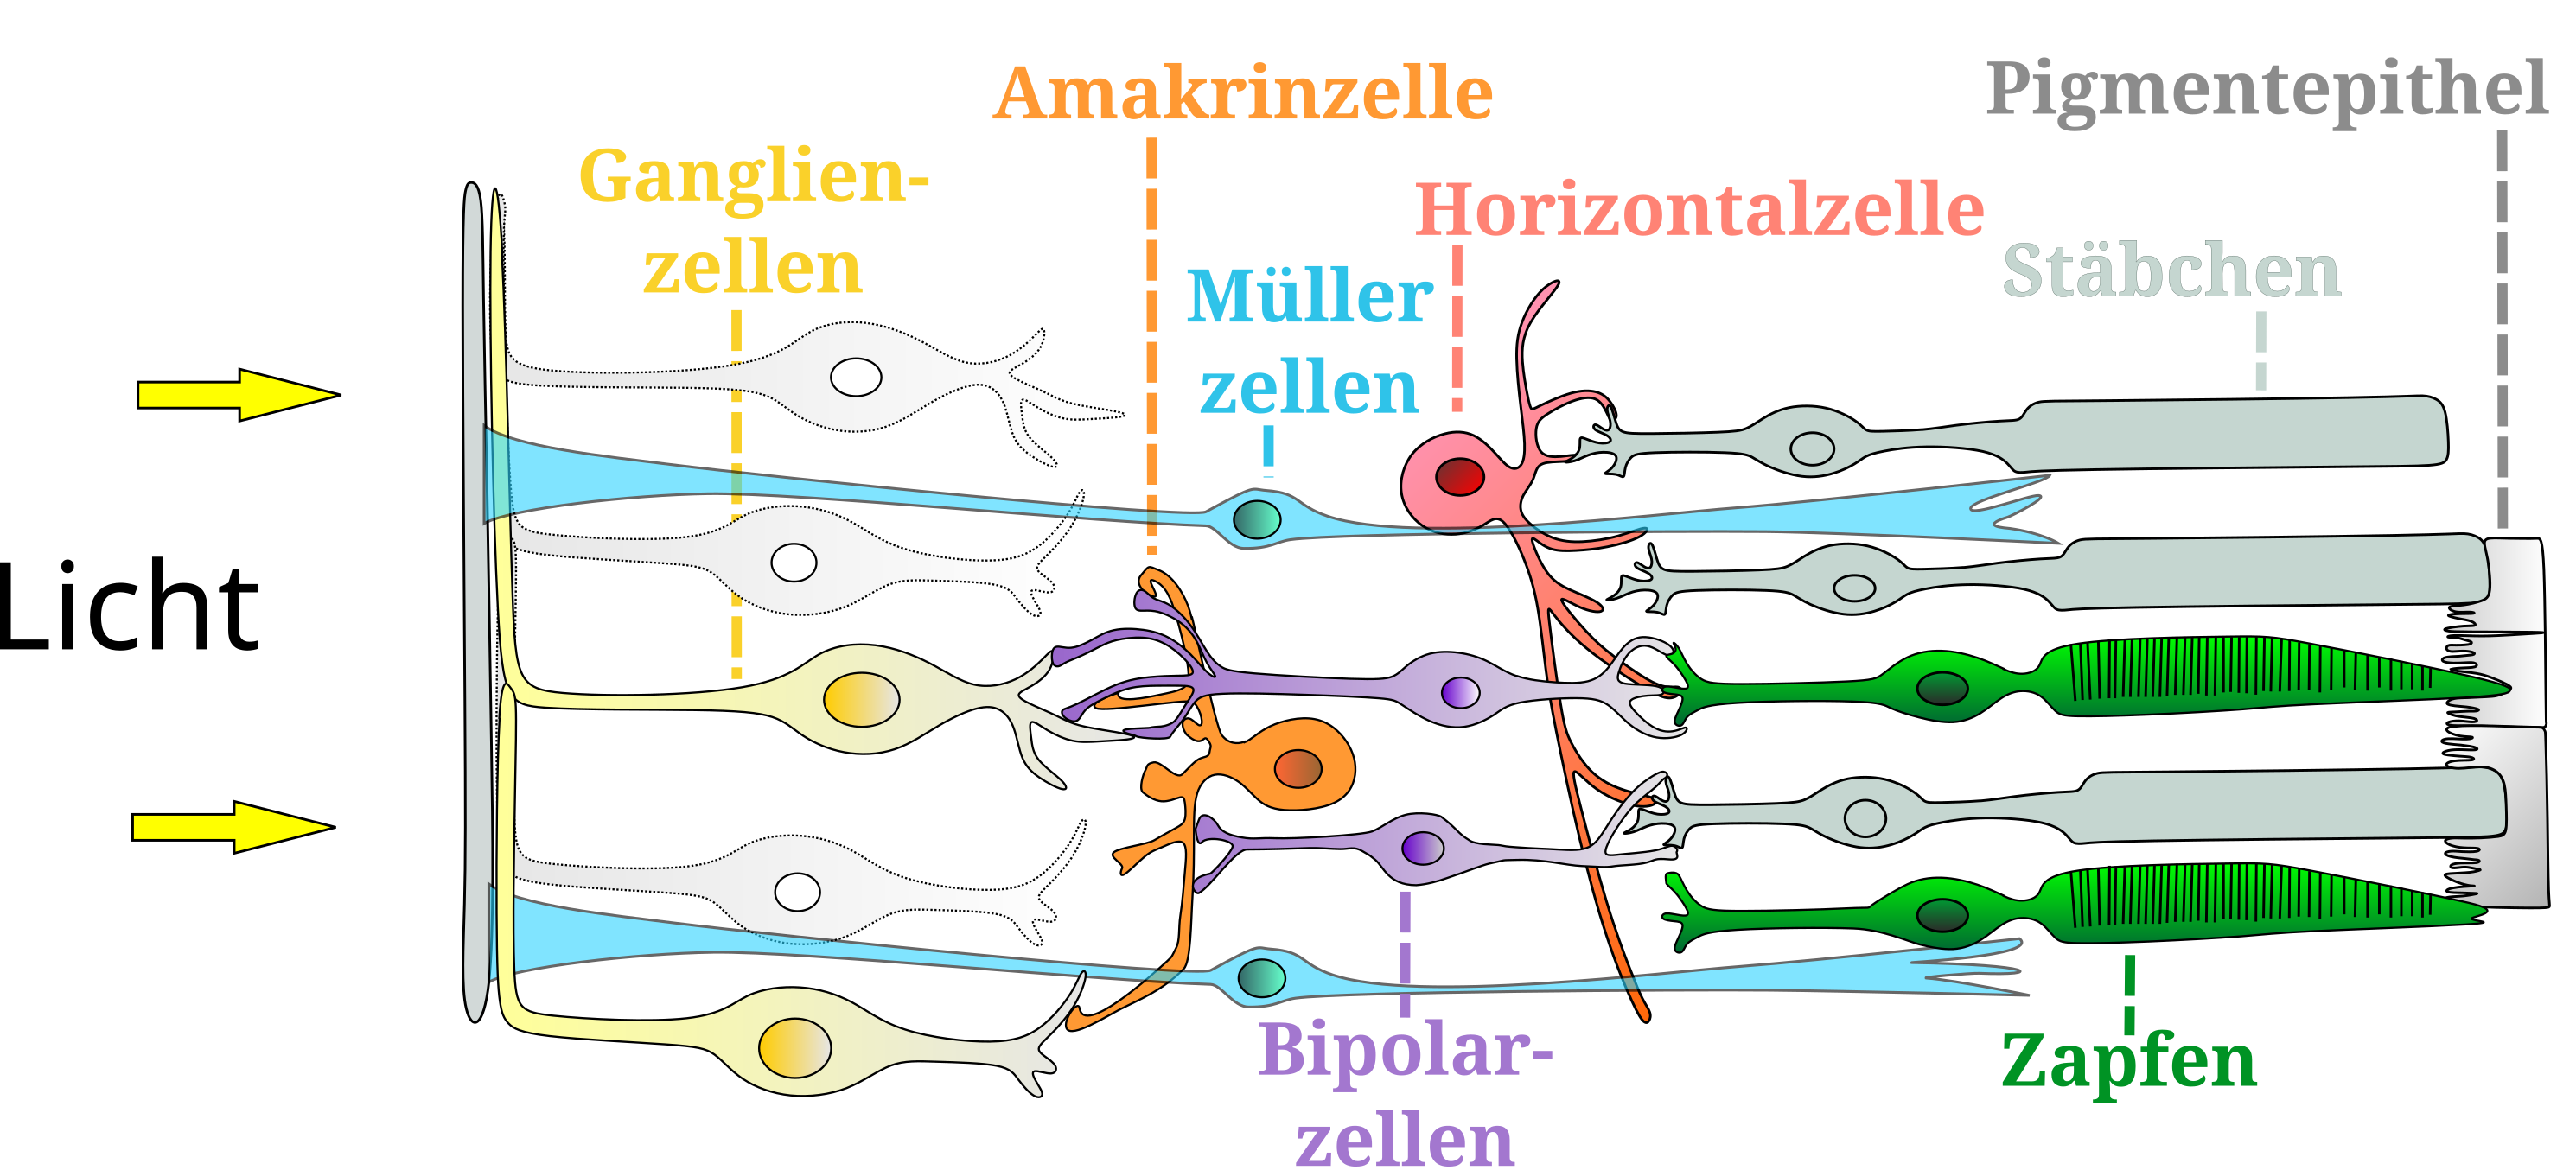
\includegraphics[width=\textwidth]{Retina_de.png}
\end{center}
\end{frame}


%% Auflösung: Bild on/off ganglien
\begin{frame}{IMPP Frage}
\begin{center}
    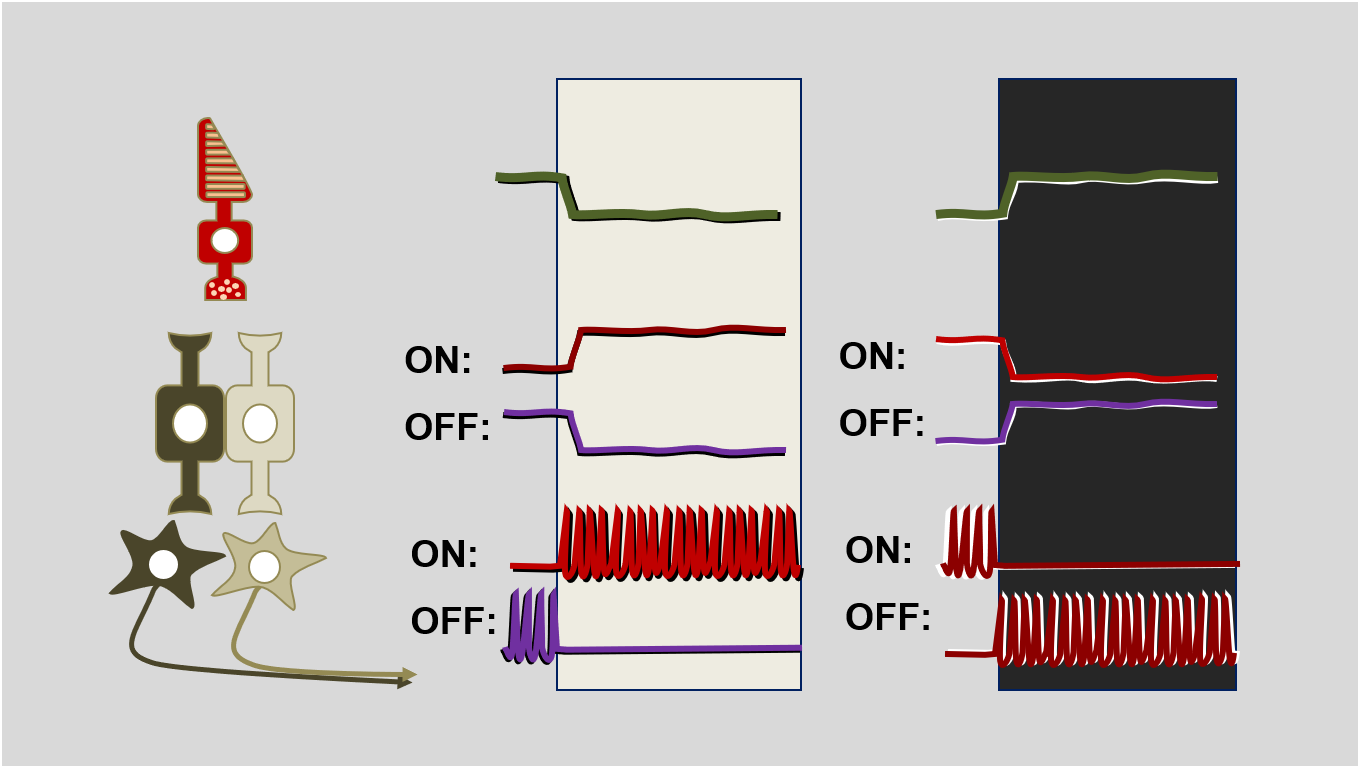
\includegraphics[width=\textwidth]{on_off_bipolarzellen.png}
\end{center}

Off-Ganglienzellen erhalten Signale direkt von Bipolarzellen, die  über ionotrope Glutamatrezeptoren direkt von Zapfen depolarisiert werden.

\end{frame}


%%%%%%%%%%%%%%%%%%%%%%%%%%%%%%%%%%%%%%%%%%%%%%%%%%%%%%%%%%%%%%%%%%%%%%%
%%%% Sehen bei Tag und Nacht: Farbensehen 24-27, Adaptation 50-54
%%%%%%%%%%%%%%%%%%%%%%%%%%%%%%%%%%%%%%%%%%%%%%%%%%%%%%%%%%%%%%%%%%%%%%%

%% Farbensehen

\begin{frame}{Aber wir wollten ja noch über Farben reden}

\begin{center}
    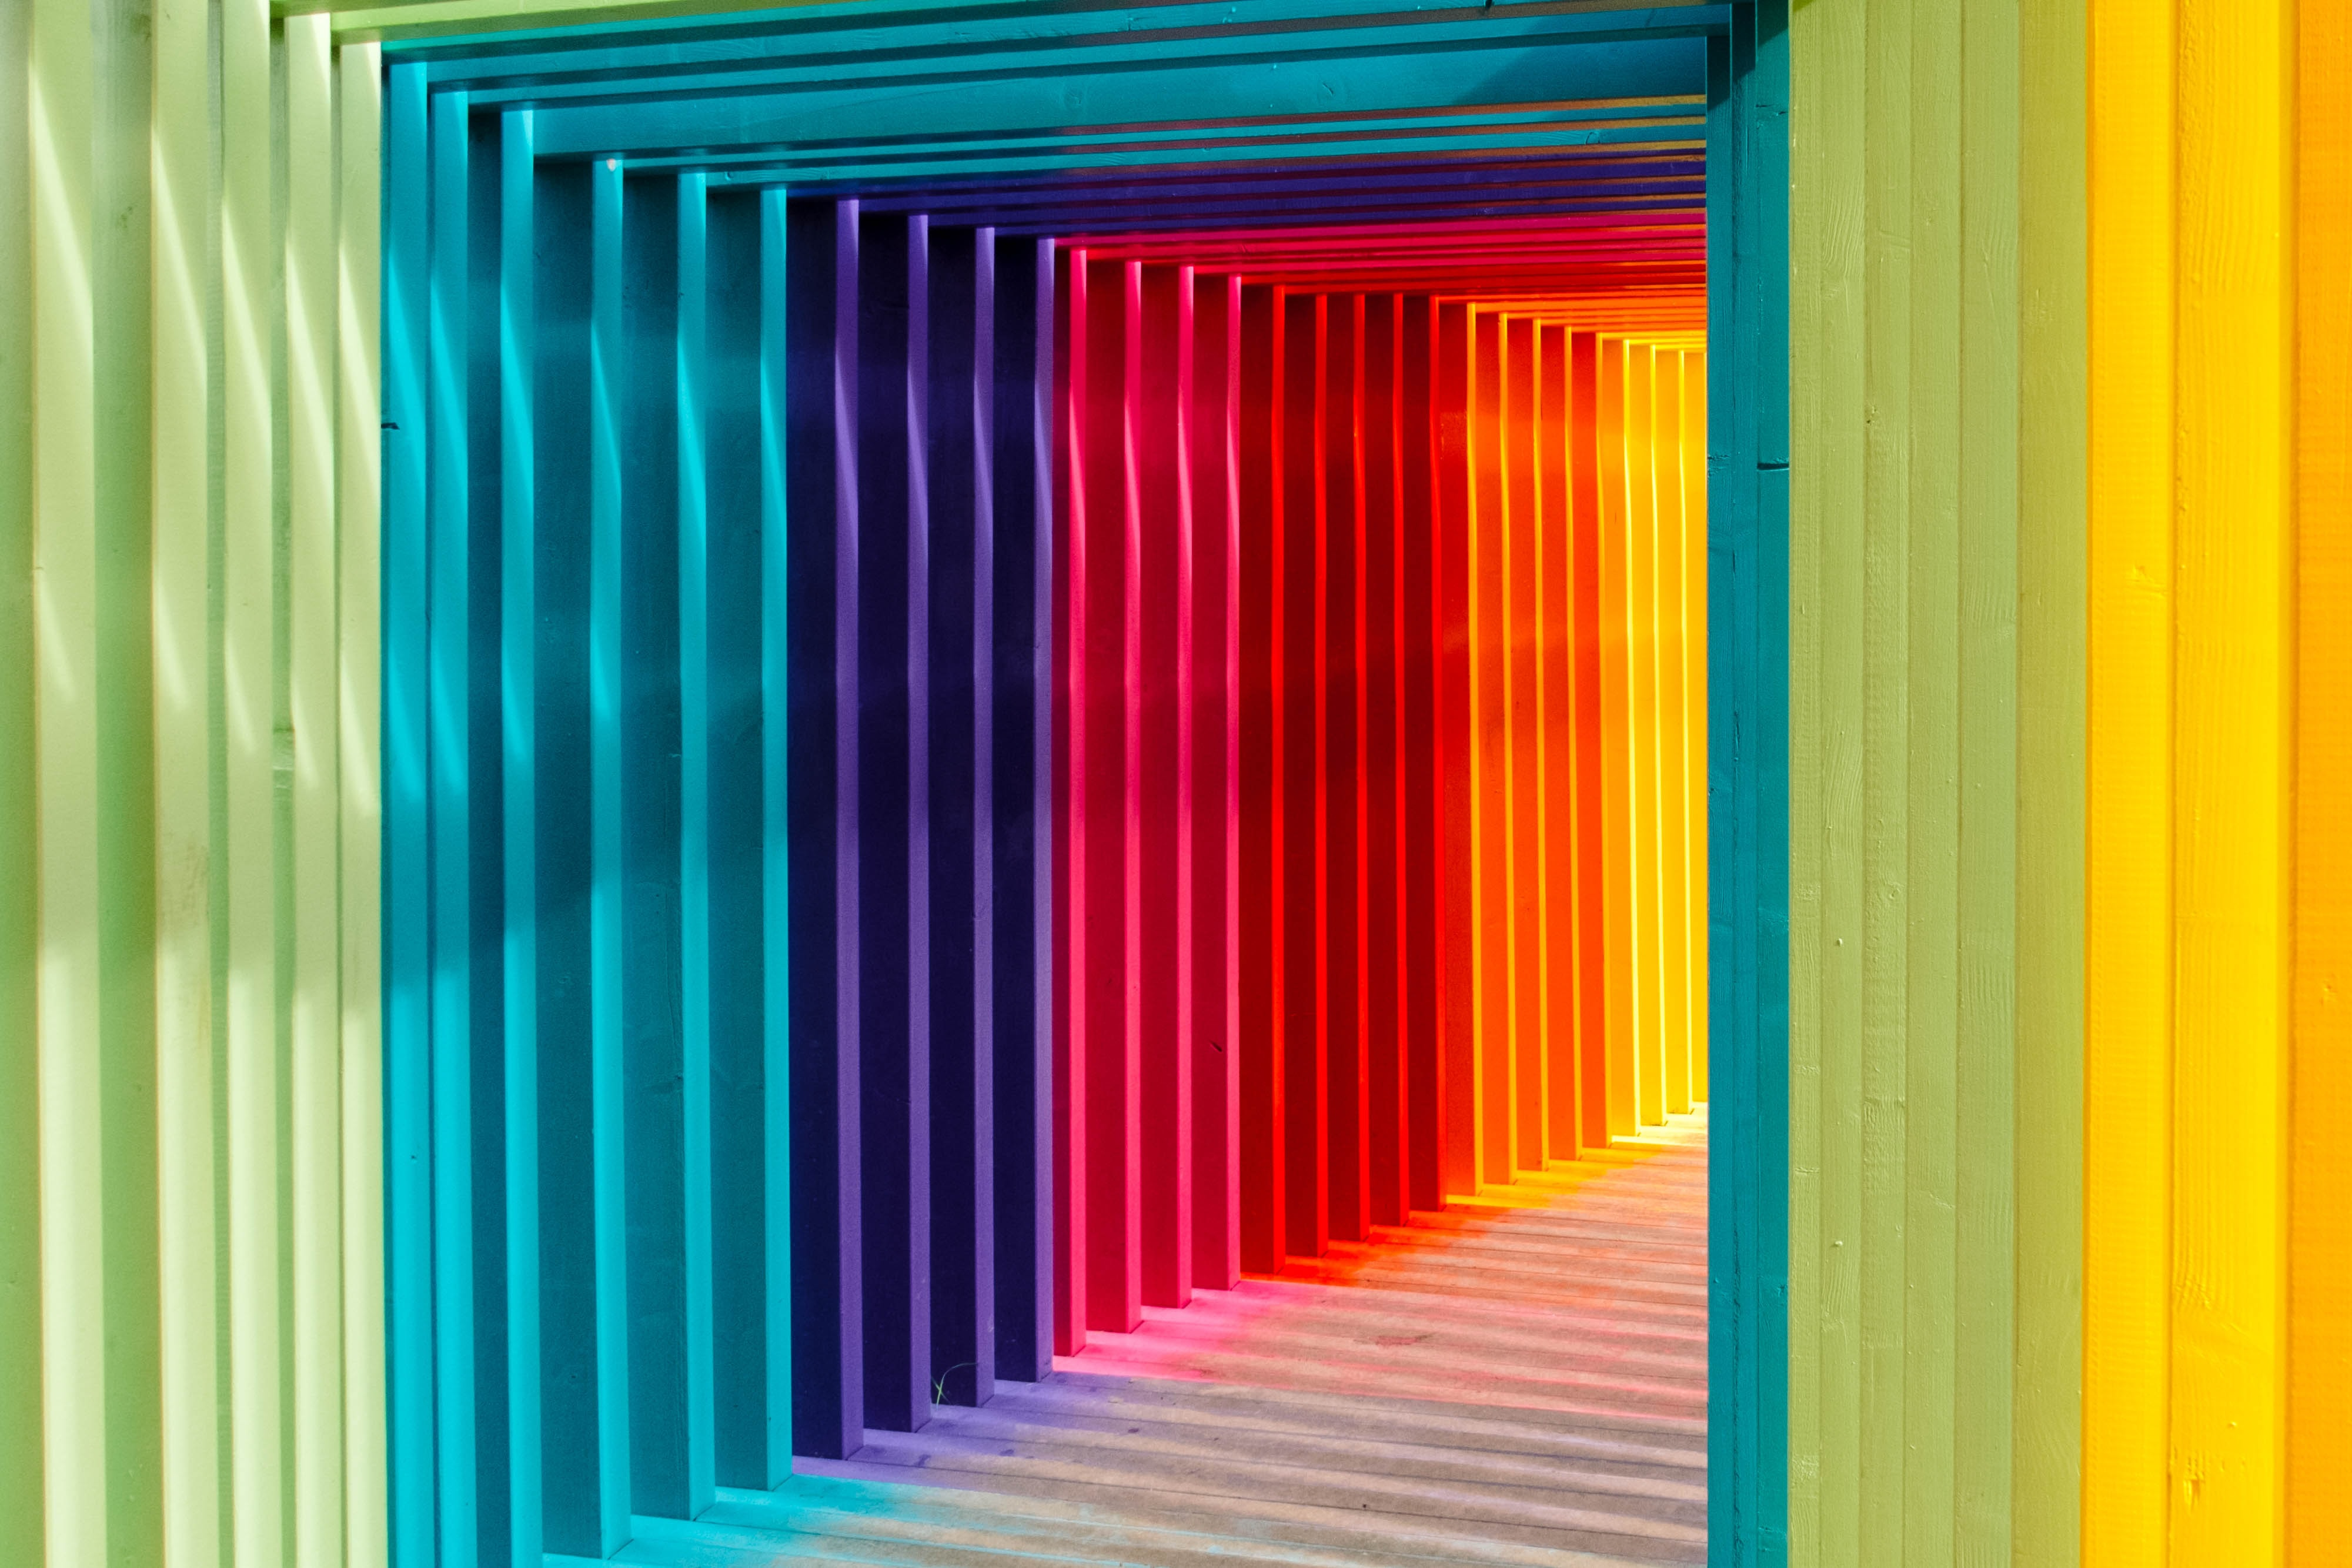
\includegraphics[width=\textwidth]{robert-katzki-jbtfM0XBeRc-unsplash.jpg}
\end{center}
    
\end{frame}

\begin{frame}{Warum ermöglichen Zapfen das Farbensehen?}

Die drei verschiedenen Zapfentypen exprimieren verschiedene Opsine, die jeweils bei unterschiedlichen Wellenlängen ihr Erregungsmaximum haben. Eine bestimmte Wellenlänge regt verschiedene Zapfentypen in unterschiedlichem Ausmaß an, daraus kann die Farbe im Gehirn ``errechnet'' werden. 

\begin{center}
        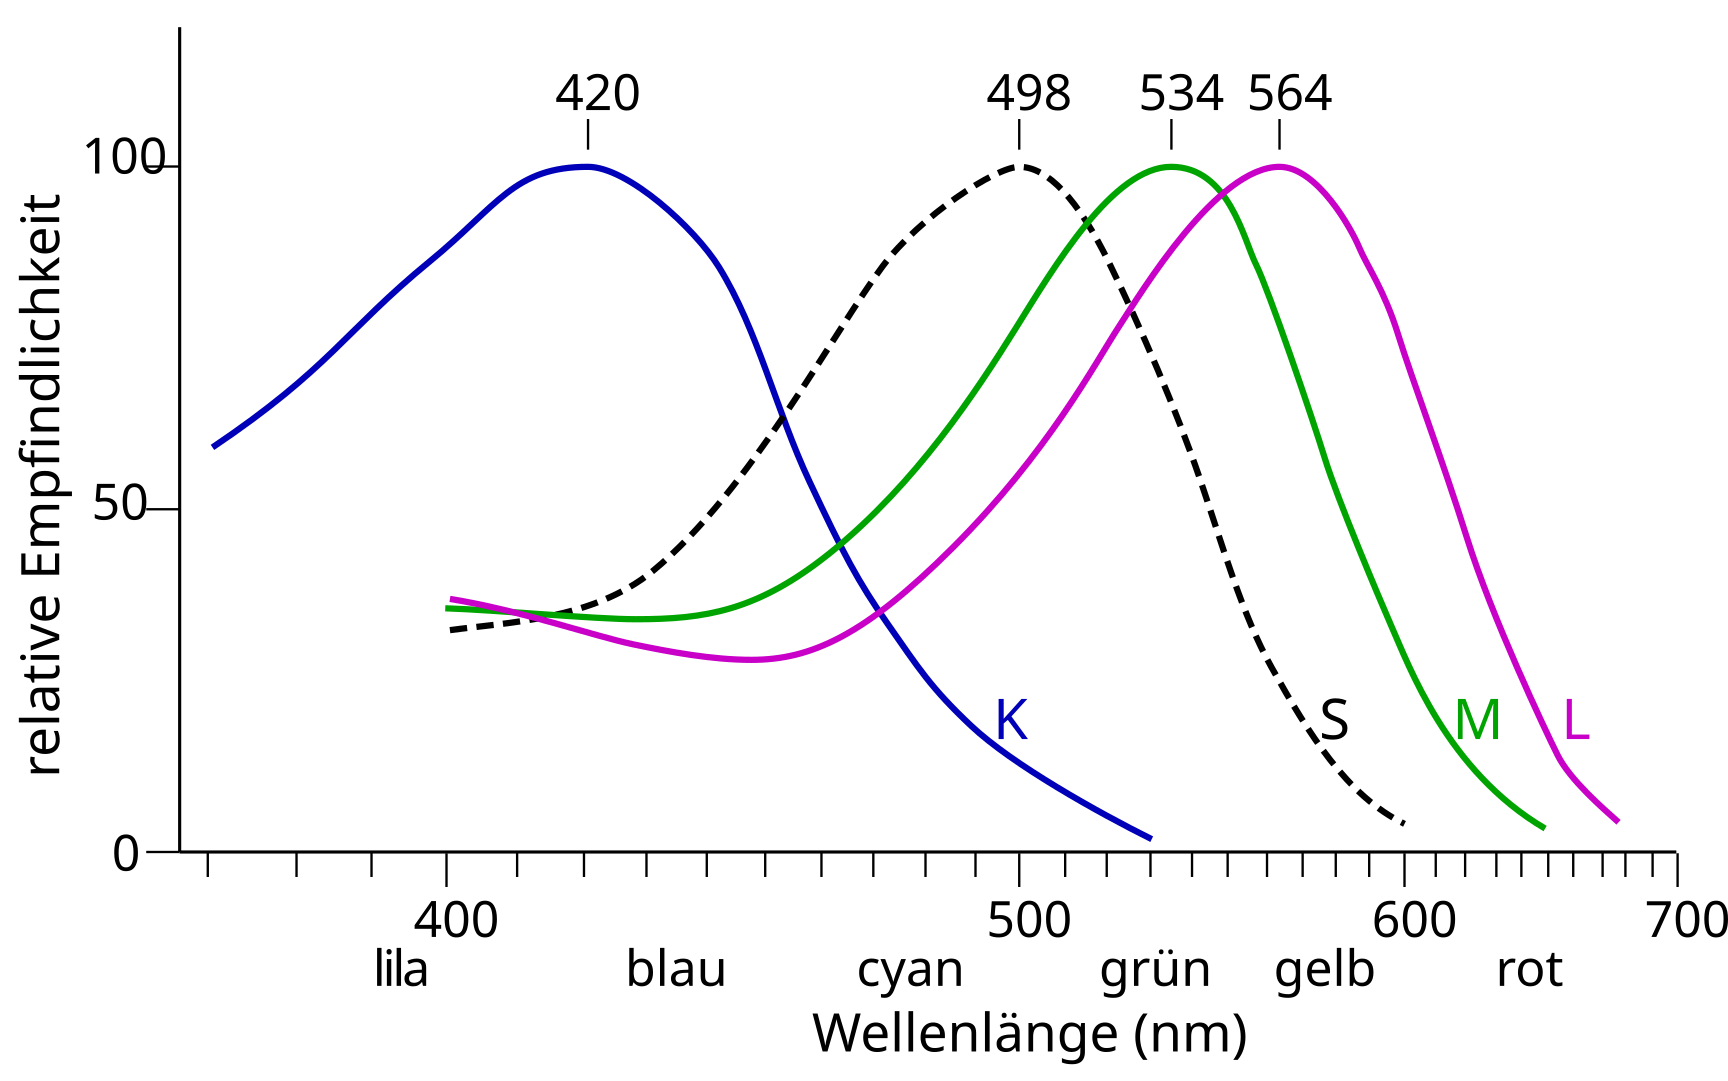
\includegraphics[width=0.7\textwidth]{Cone-response-de.png}
    \end{center}
    
\end{frame}


\begin{frame}{Anomalien des Farbensehens}

Farbschwächen und Farbenblindheit treten auf, wenn bestimmte Zapfen unterrepräsentiert oder gar nicht vorhanden sind. Gene für L- und M-Opsine liegen auf dem X-Chromosom, daher sind Störungen des Farbensehens bei Männern häufiger als bei Frauen. \\[0.5 cm]

\pause

Namensgenerator: \\[0.5 cm]


\begin{tabular}{lllll}
rot (1)    & prot- & \\
            &       & & -anomalie &  (Schwäche)\\
grün (2)    & deuter-  &&\\
            &           & \qquad& -anopie & (Blindheit) \\
blau (3)     & trit- \\&
\end{tabular}

%% spoiler alert
Beispiel: Schwäche der Blauzapfen: \pause Tritanomalie
%% end spoiler alert

\pause

Achromatopsie: Überhaupt kein Farbempfinden, praktisch nur Stäbchensystem (extrem selten)
\end{frame}

%% Example colour chart: downloaded
\begin{frame}{Beispiel: Universelles Design für Farbenblindheit}

\begin{center}
    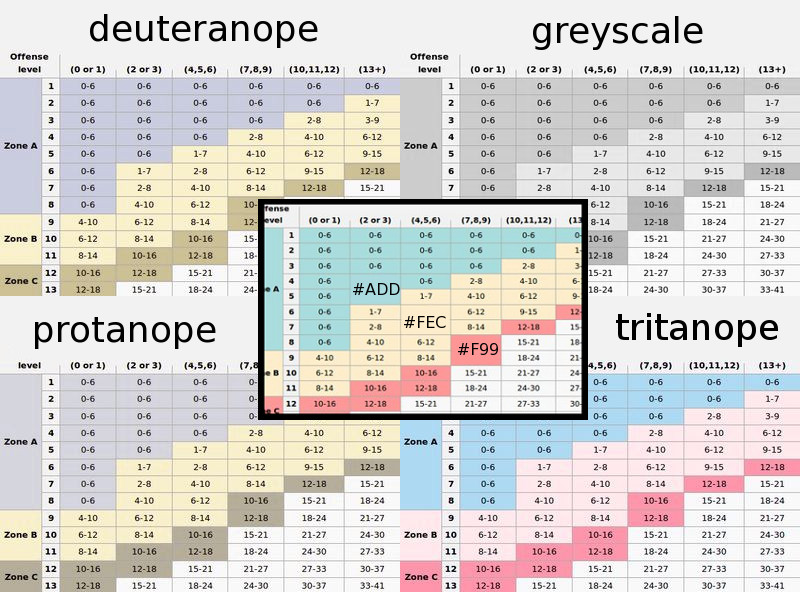
\includegraphics[width=0.8\textwidth]{Safe_Chart_Colors-F99-FEC-ADD.jpg}
\end{center}
    
\end{frame}


%% Adaptation

\begin{frame}{Aber was machen eigentlich die Stäbchen?}

Wir erinnern uns: Stäbchen sind: \dots

\pause

\begin{itemize}
    \item 
    extrem lichtsensitiv
    \item
    wenig auflösend
    \item
    nicht am Farbensehen beteiligt
\end{itemize}

\pause

2 verschiedene Systeme: Photopisches Sehen (Zapfen) am Tag, skotopisches Sehen (Stäbchen) in der Dunkelheit
    
\end{frame}

\begin{frame}{Wie signalisieren Stäbchen?}
    
    Stäbchen haben nur On-Bipolarzellen. Sie signalisieren nicht direkt an Ganglienzellen, sondern "hijacken" das Zapfensystem: Über Stäbchen-Amakrine aktivieren sie Zapfen-On-Bipolarzellen und inhibieren Zapfen-Off-Bipolarzellen
    
    \begin{center}
        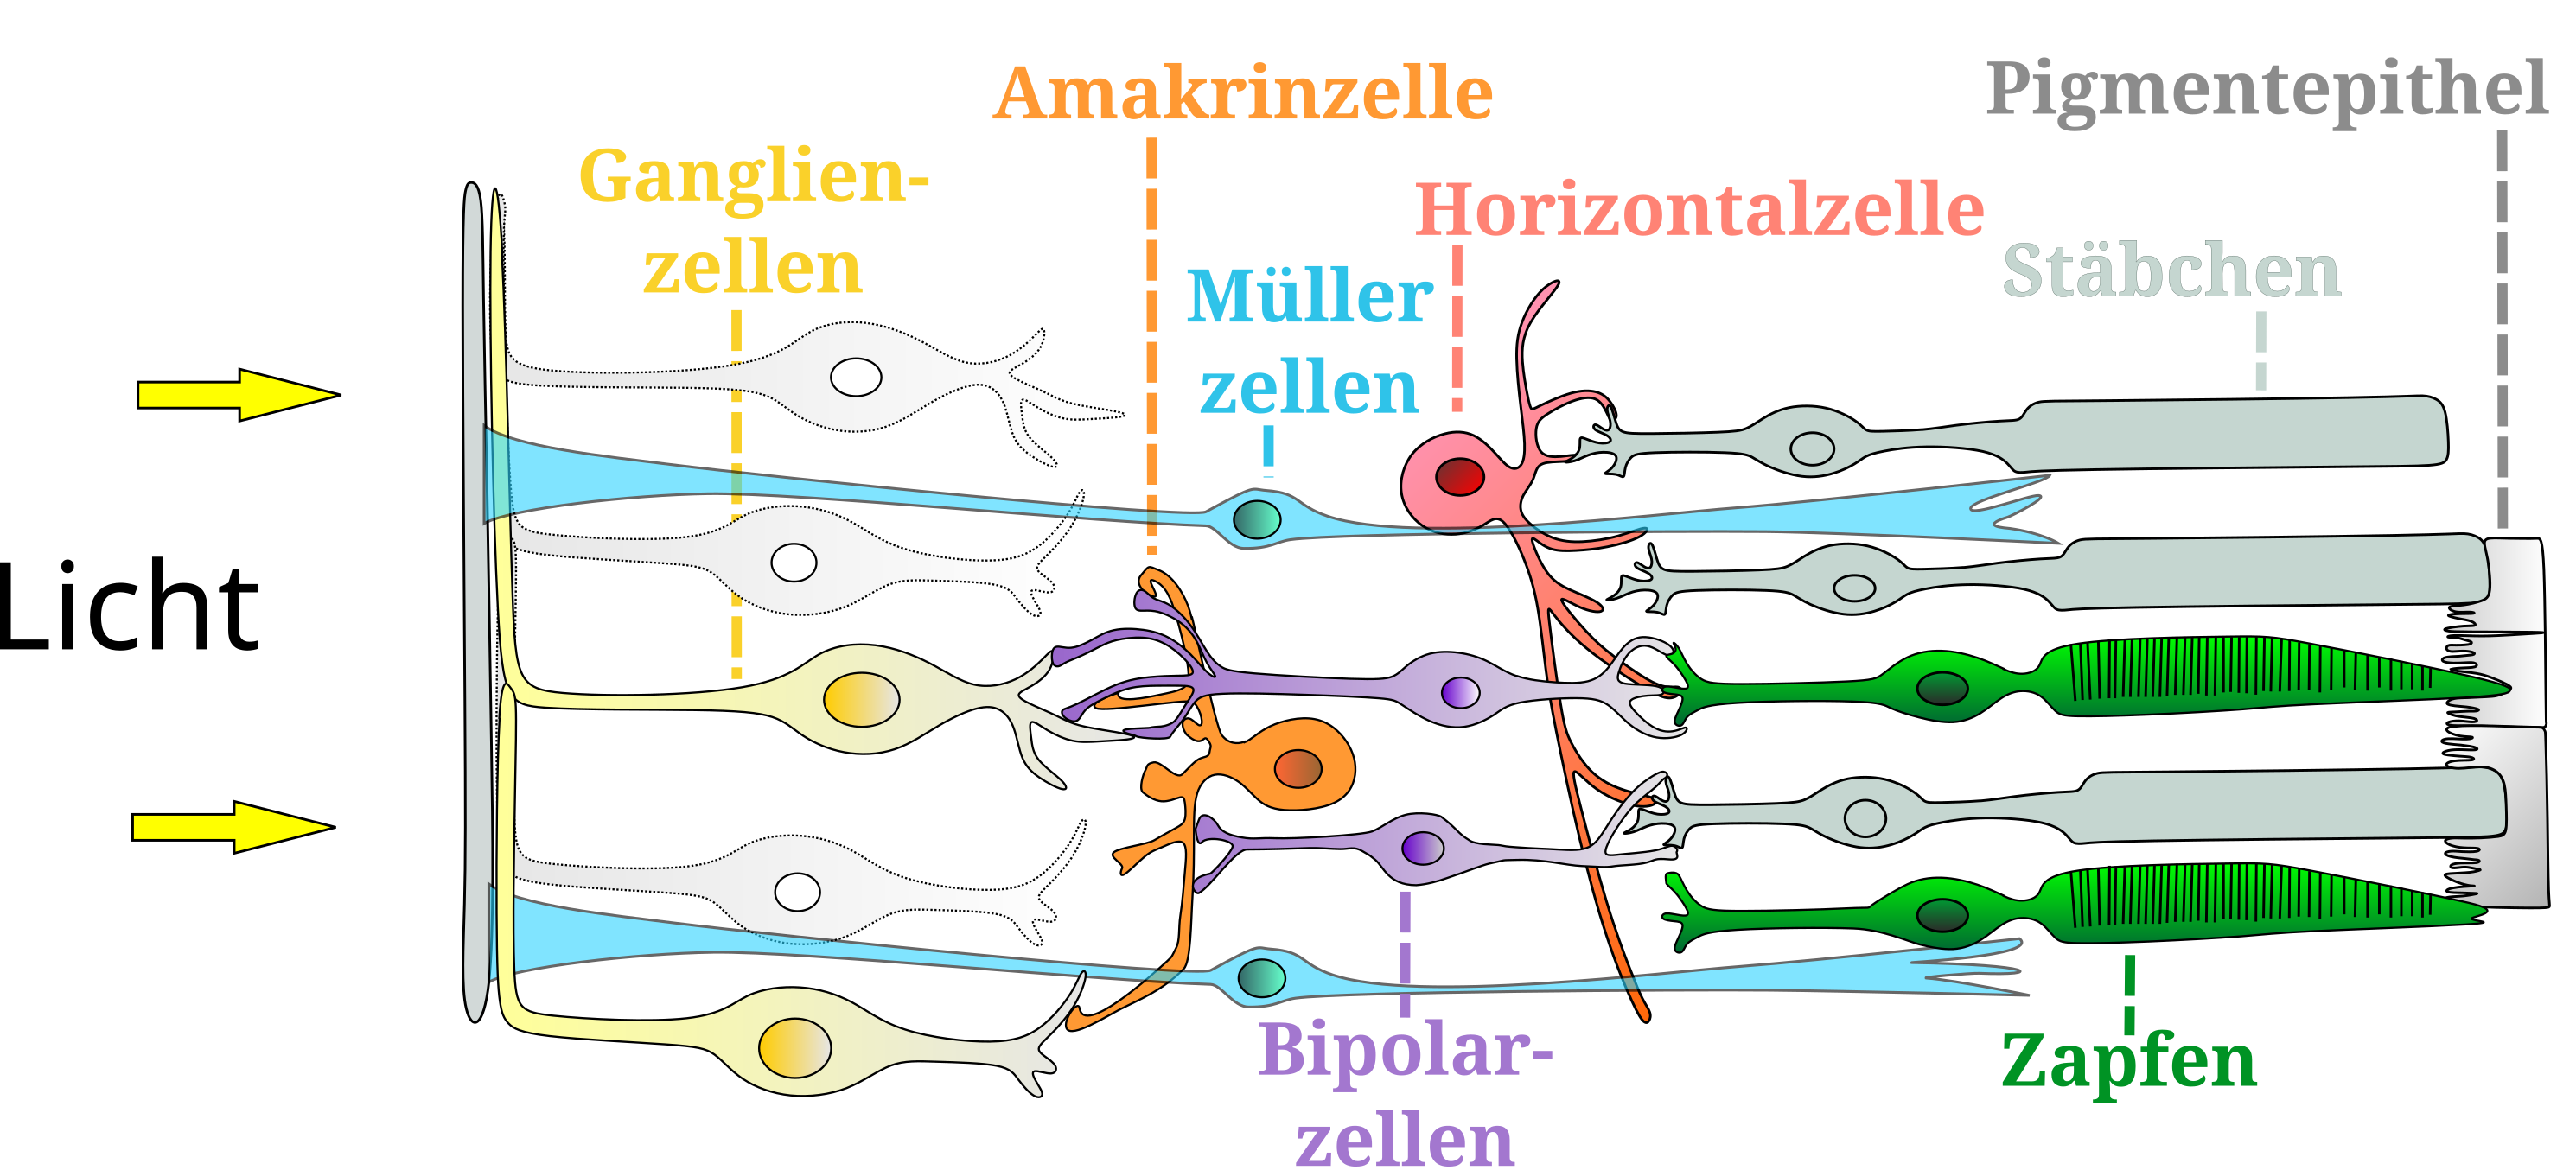
\includegraphics[width=\textwidth]{Retina_de.png}
    \end{center}
    
\end{frame}

%% Adapation Hell/Dunkel



\begin{frame}{Hell-Dunkel Adaptation beruht auf mehreren Prozessen}

\begin{itemize}
    \item 
    Pupillenreflex
\item
Veränderung der Signalkaskaden, z.B. längere Lebenszeit von aktiviertem Metarhodopsin
\item
Umschalten von Zapfen-System auf Stäbchen System (bei Licht werden Stäbchen-Amakrine von Zapfen-Amakrinen gehemmt; diese Hemmung wird bei Dunkelheit aufgehoben)
\item
Vergrößerung der rezeptiven Felder (geht auf Kosten von Sehschärfe, bewerkstelligt aber größere Sensitivität)
\end{itemize}

    
\end{frame}


\begin{frame}{Hell-Dunkel Adaptation beruht auf mehreren Prozessen}

\begin{center}
    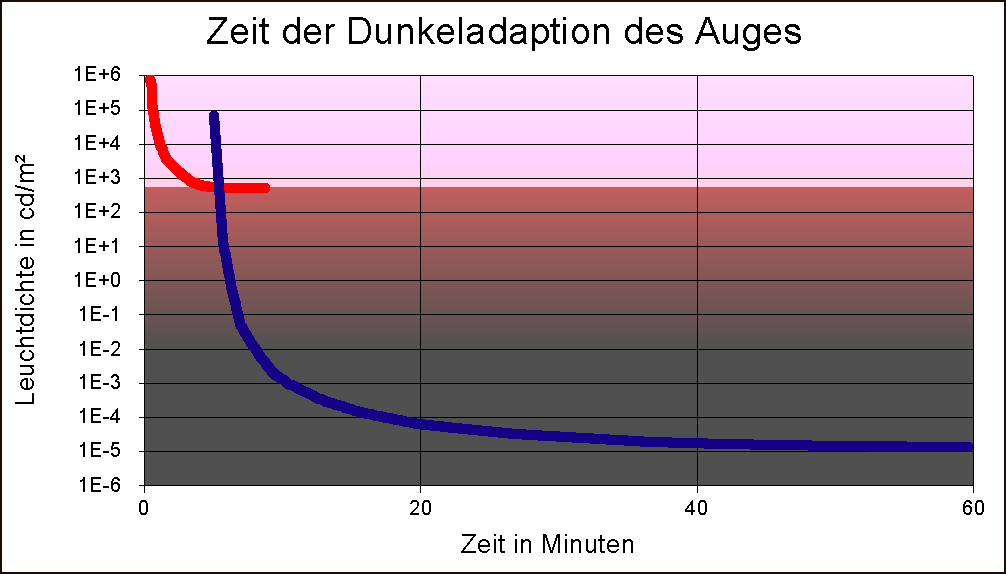
\includegraphics[width=\textwidth]{Hdadaptrp.png}
    \end{center}
    
\end{frame}


%% IMPP Frage, Einfügen an geeignetem ort

\begin{frame}{IMPP Frage}

Welche Aussage zur Wellenlänge (in nm) des Absorptionsmaximums der Stäbchen in der Netzhaut trifft typischerweise zu?

\begin{description}
\item[A.] Sie ist größer als die der Grünzapfen (M-Zapfen)
\item[B.] Sie ist größer als die der Rotzapfen (L-Zapfen) 
\item[C.] Sie ist kleiner als die der Blauzapfen (K-Zapfen) 
\item[D.] Sie liegt zwischen der der Blauzapfen (K-Zapfen) und der der Grünzapfen (M-Zapfen) %% richtig
\item[E.] Sie liegt zwischen der der Grünzapfen (M-Zapfen) und der der Rotzapfen (L-Zapfen) 
\end{description}

    
\end{frame}

%% Auflösung: Bild Cone-response.svg
\begin{frame}{IMPP Frage}
    
    \begin{center}
        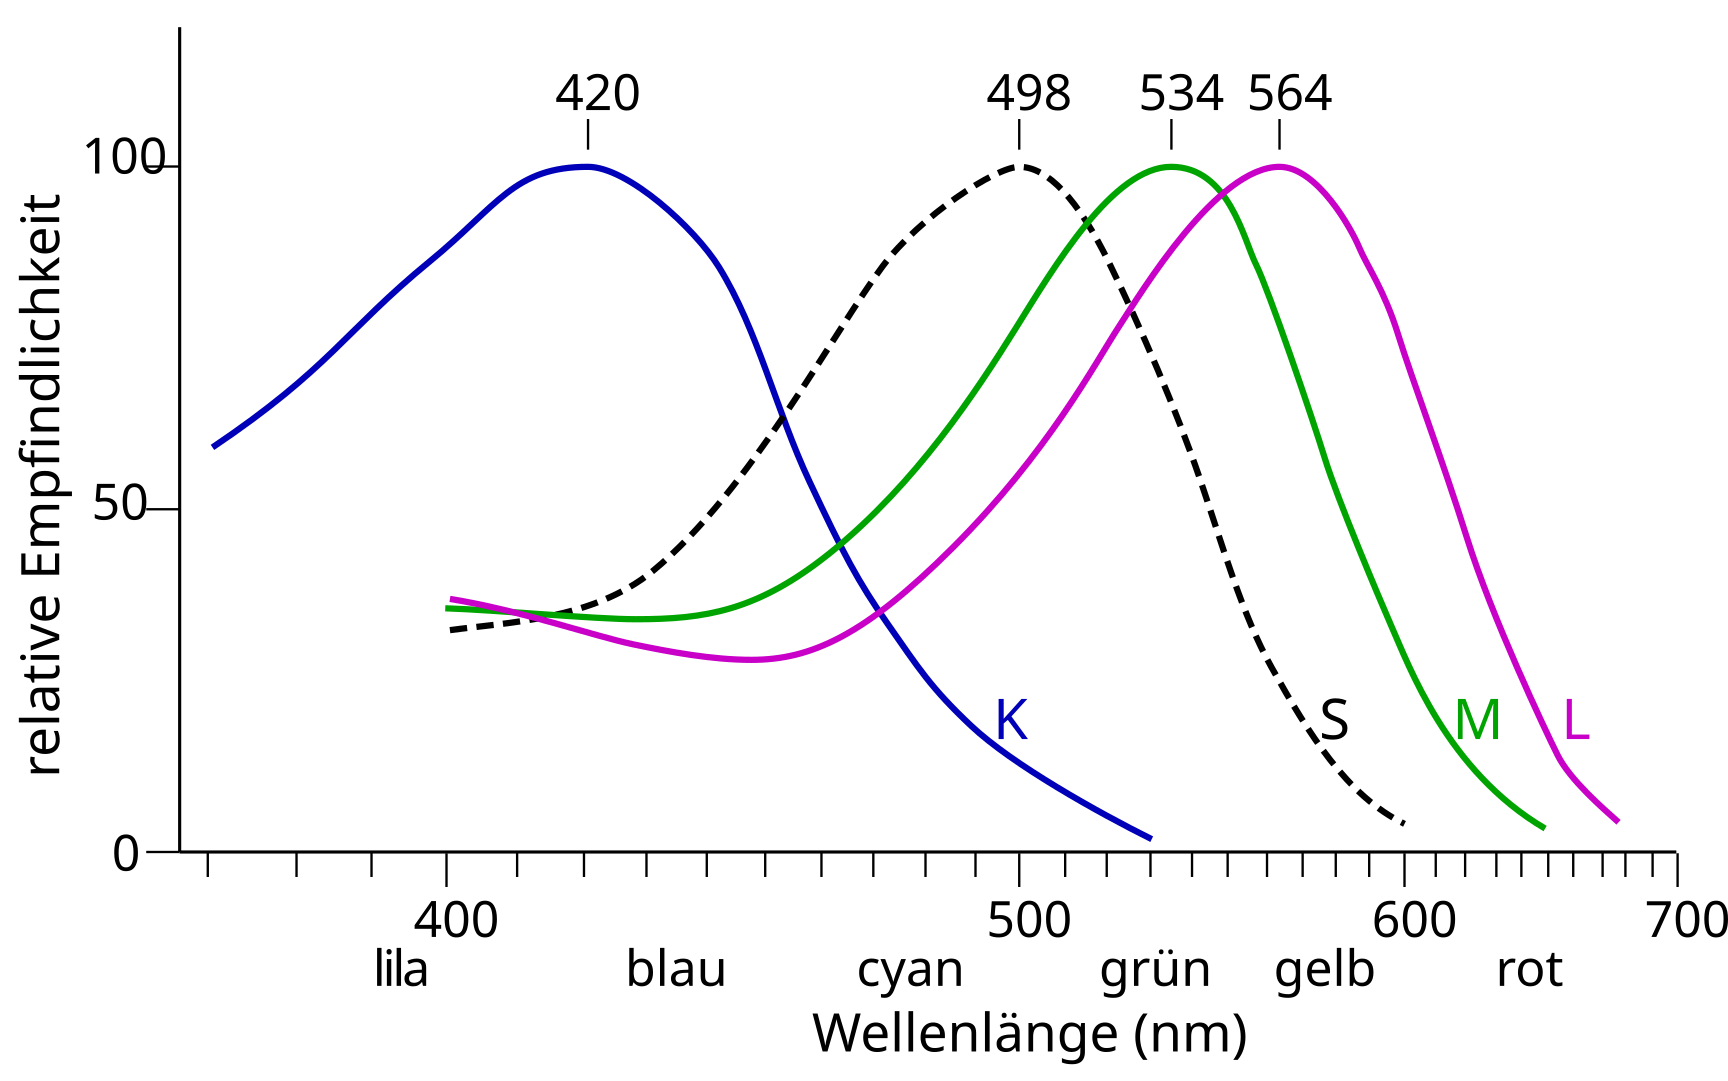
\includegraphics[width=\textwidth]{Cone-response-de.png}
    \end{center}
    
\end{frame}








%%%%%%%%%%%%%%%%%%%%%%%%%%%%%%%%%%%%%%%%%
%% Wahrnehmungsbahn: Afferente Nerven
%%%%%%%%%%%%%%%%%%%%%%%%%%%%%%%%%%%%%%%%%

%% Afferente Nerven generelles Bild
\begin{frame}{Die Sehbahn}

\begin{cener}
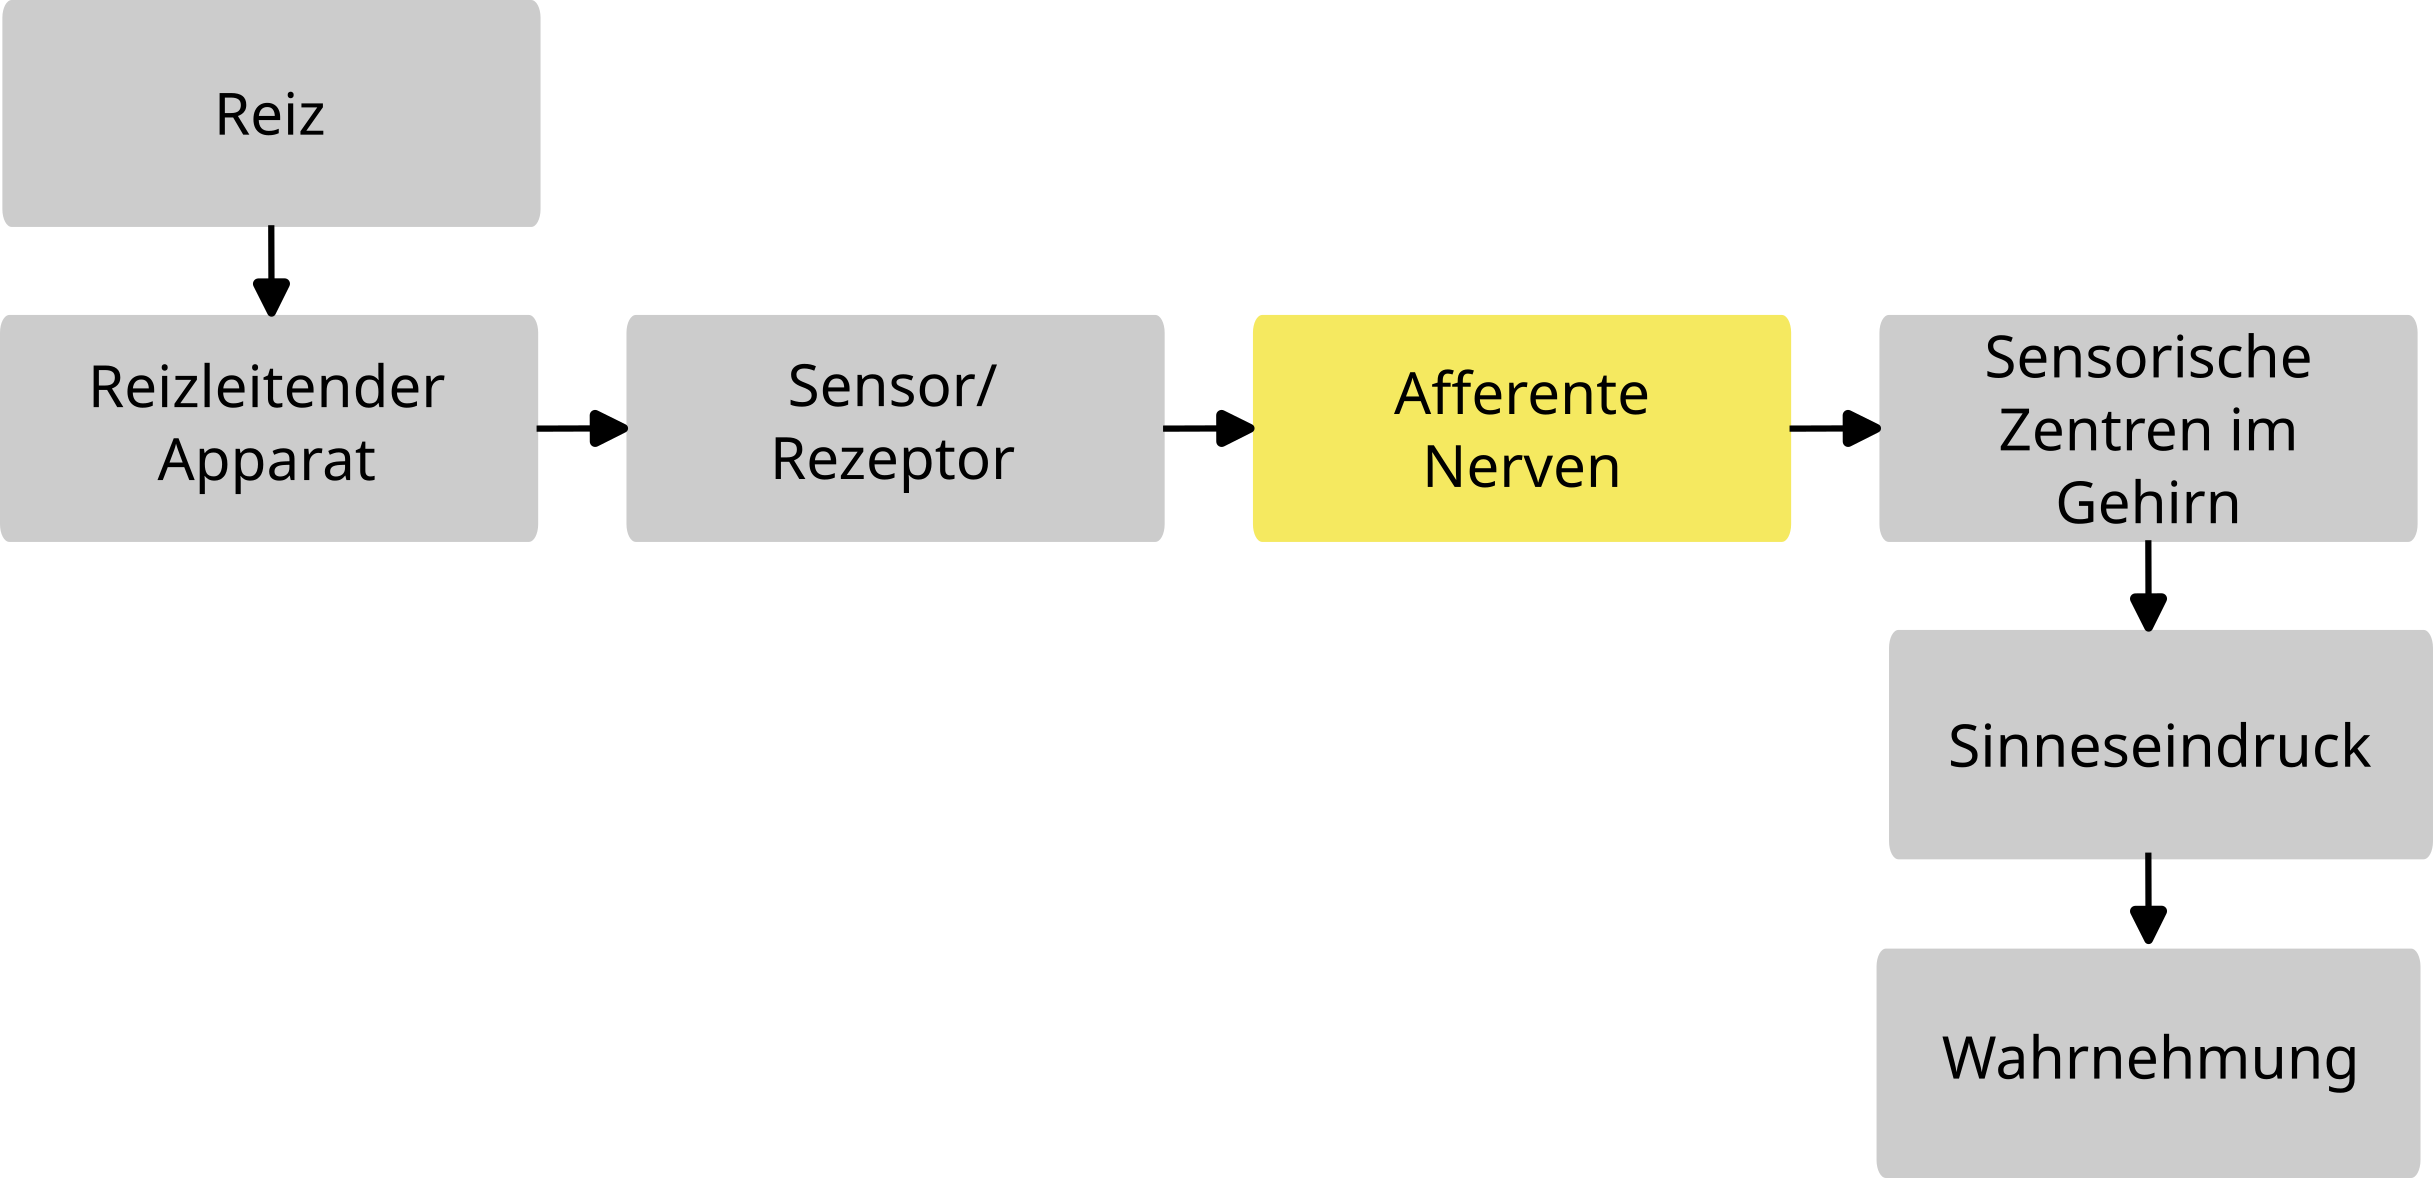
\includegraphics[width=\textwidth]{wahrnehmungsprozess_ohne_beispiel_bahnen.png}
\end{cener}

\end{frame}


%% Verlauf der Sehbahn 58
%% Have image

\begin{frame}{Die Sehbahn}

\begin{center}
    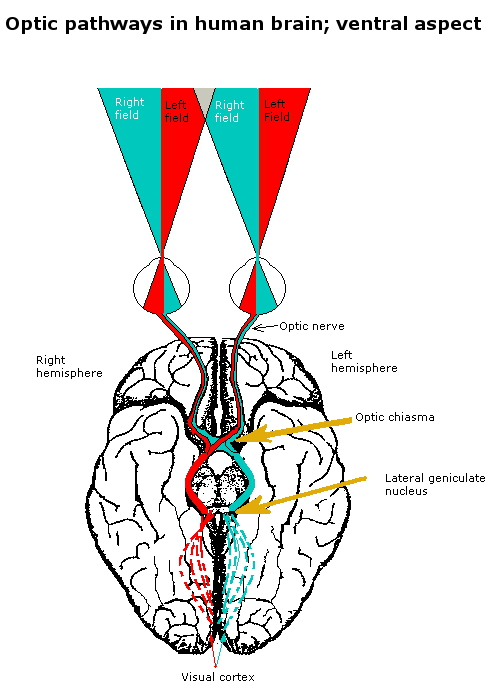
\includegraphics[width=0.5\textwidth]{Optic_processing_human_brain.jpg}
\end{center}
\end{frame}



\begin{frame}{Die Sehbahn}

\begin{columns}[c]

\begin{column}{6cm}
\begin{center}
        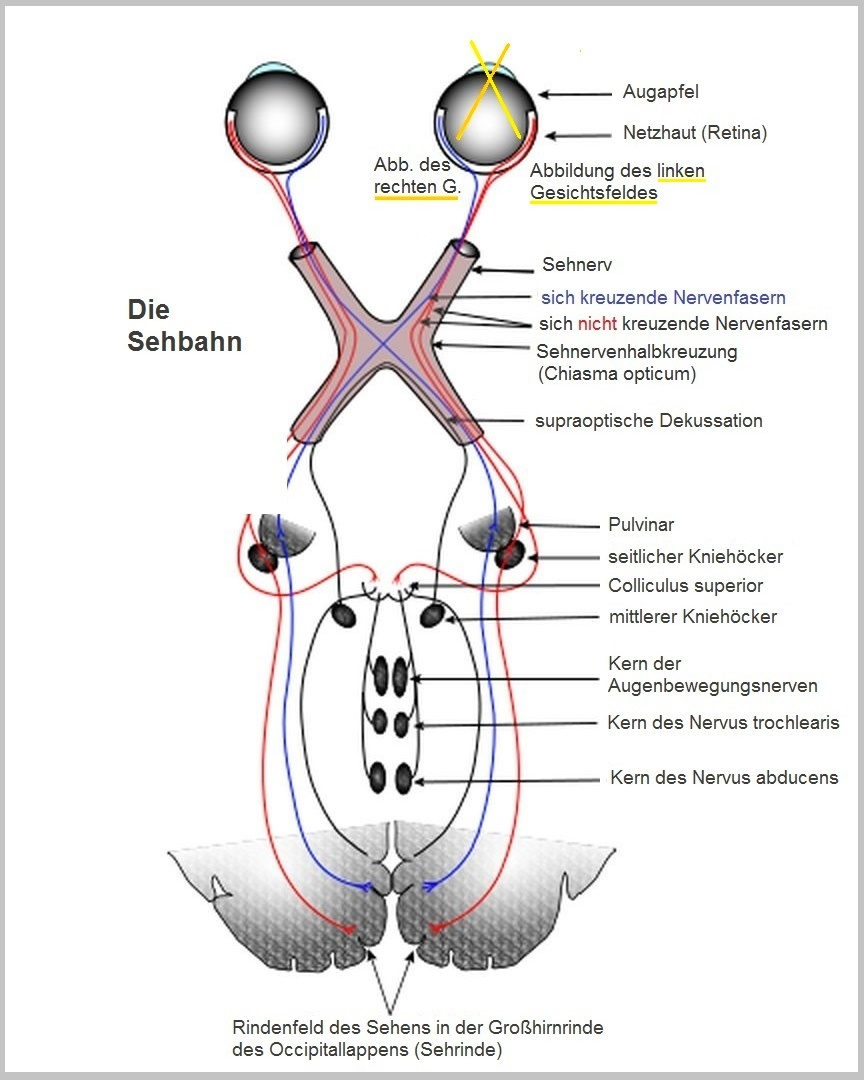
\includegraphics[width=\textwidth]{Sehbahn_mit_Chiasma_opticum.jpg}
\end{center}

\end{column}


\begin{column}{6cm}
\begin{itemize}
    \item 
    Im optischen Chiasma kreuzen die Nervenfasern aus dem nasalen (aber nicht aus dem temporalen) Teil der Netzhaut. Daraus entsteht eine Abbildung der linken Hälfte des Gesichtsfeldes in der rechten Hemisphäre und umgekehrt
    \pause
    \item
    Die meisten Fasern werden im Corpus geniculatum laterale im Thalamus umgeschaltet zur primären Sehrinde. 
    

\end{itemize}
\end{column}


\end{columns}

\end{frame}


\begin{frame}{Die Sehbahn}

\begin{columns}[c]

\begin{column}{6cm}
\begin{center}
        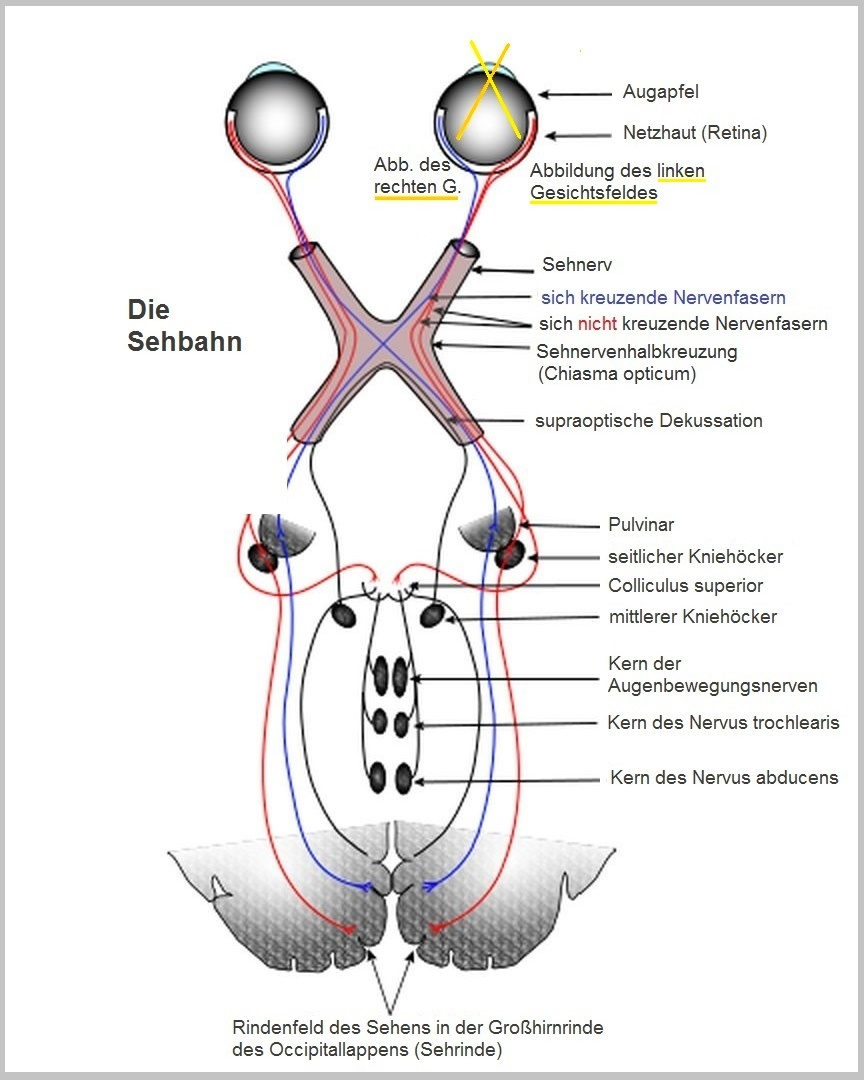
\includegraphics[width=\textwidth]{Sehbahn_mit_Chiasma_opticum.jpg}
\end{center}

\end{column}


\begin{column}{6cm}

 Ca. \(10\,\%\) der Fasern dienen unbewussten Prozessen. Sie ziehen ohne Umschaltung im Corpus geniculatus laterale direkt in andere Regionen: 
   
\begin{itemize}
    \item 
    Nucleus superchiasmaticus für circadiane Rhythmik
    \item
Nuclei praetectales für Pupillenreflexe und Akkommodation 

\end{itemize}
\end{column}


\end{columns}

\end{frame}


%%%%%%%%%%%%%%%%%%%%%%%%%%%%%%%%%%%%%%%%%
%%%% Gesichtsfeld, Skotome, Perimetrie 57, 59
%%%%%%%%%%%%%%%%%%%%%%%%%%%%%%%%%%%%%%%%%

\begin{frame}{Gesichtsfeld}

\begin{columns}[c]

\begin{column}{5cm}
    Das Gesichtsfeld ist die Menge aller Punkte, die bei unbewegtem Kopf und mit fixiertem Auge wahrnehmbar ist. \\
    
Monokular: \(\sim 160^{\circ}\) \\
Binokular: \(\sim 190-200^{\circ}\) \\
\end{column}


\begin{column}{5cm}
\begin{center}
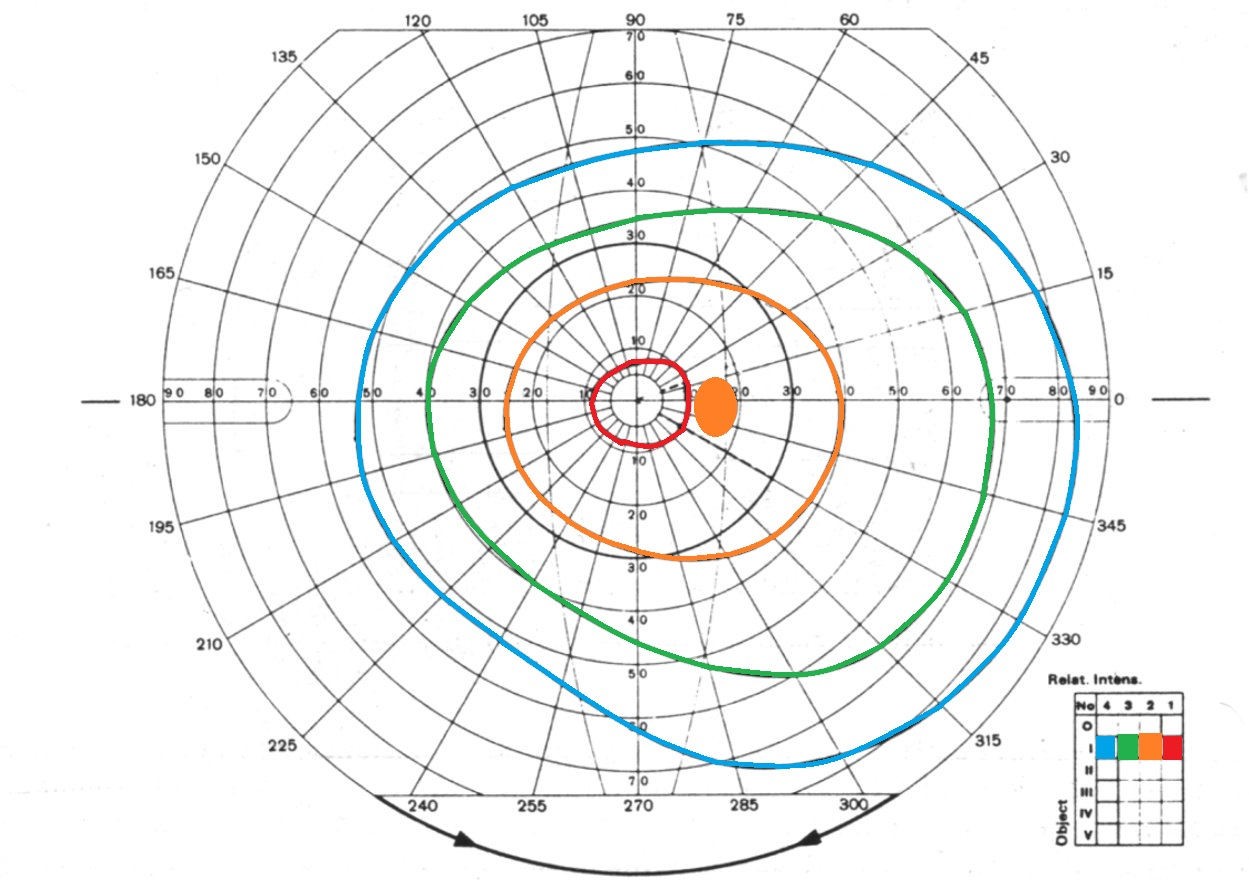
\includegraphics[width=\textwidth]{Goldmann_visual_field_record_sheet.jpg}
\end{center}
\end{column}

\end{columns}

    
\end{frame}

\begin{frame}{Das Gesichtsfeld kann mit Perimetrie vermessen werden}


\begin{cneter}
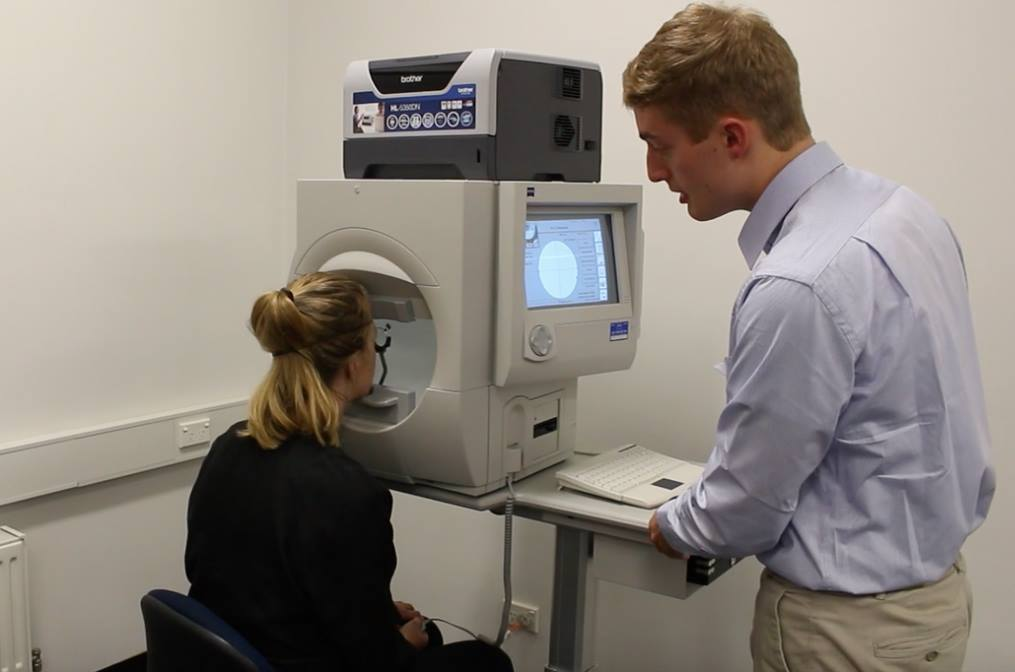
\includegraphics[width=\textwidth]{Perimetry_test.jpg}
\end{cneter}

    
\end{frame}


\begin{frame}{Ausfälle im Gesichtsfeld (Skotome) erlauben Rückschlüsse auf geschädigte Nervenbahnen}

\begin{center}
    \includegraphics<1>[width=0.6\textwidth]{Hemianopsien_raetsel.png}
    
    \includegraphics<2>[width=0.6\textwidth]{Hemianopsien_raetsel_rechts.png}

    \includegraphics<3>[width=0.6\textwidth]{Hemianopsien.png}
\end{center}


\end{frame}




%%%%%%%%%%%%%%%%%%%%%%%%%%%%%%%%%%%%%%%%%
%% Sensorische Zentren im Gehirn Sinneseindruck, Wahrnehmung
%%%%%%%%%%%%%%%%%%%%%%%%%%%%%%%%%%%%%%%%%

%% Überblick Gehirn
\begin{frame}{Sensorische Zentren im Gehirn}
    
    \begin{center}
        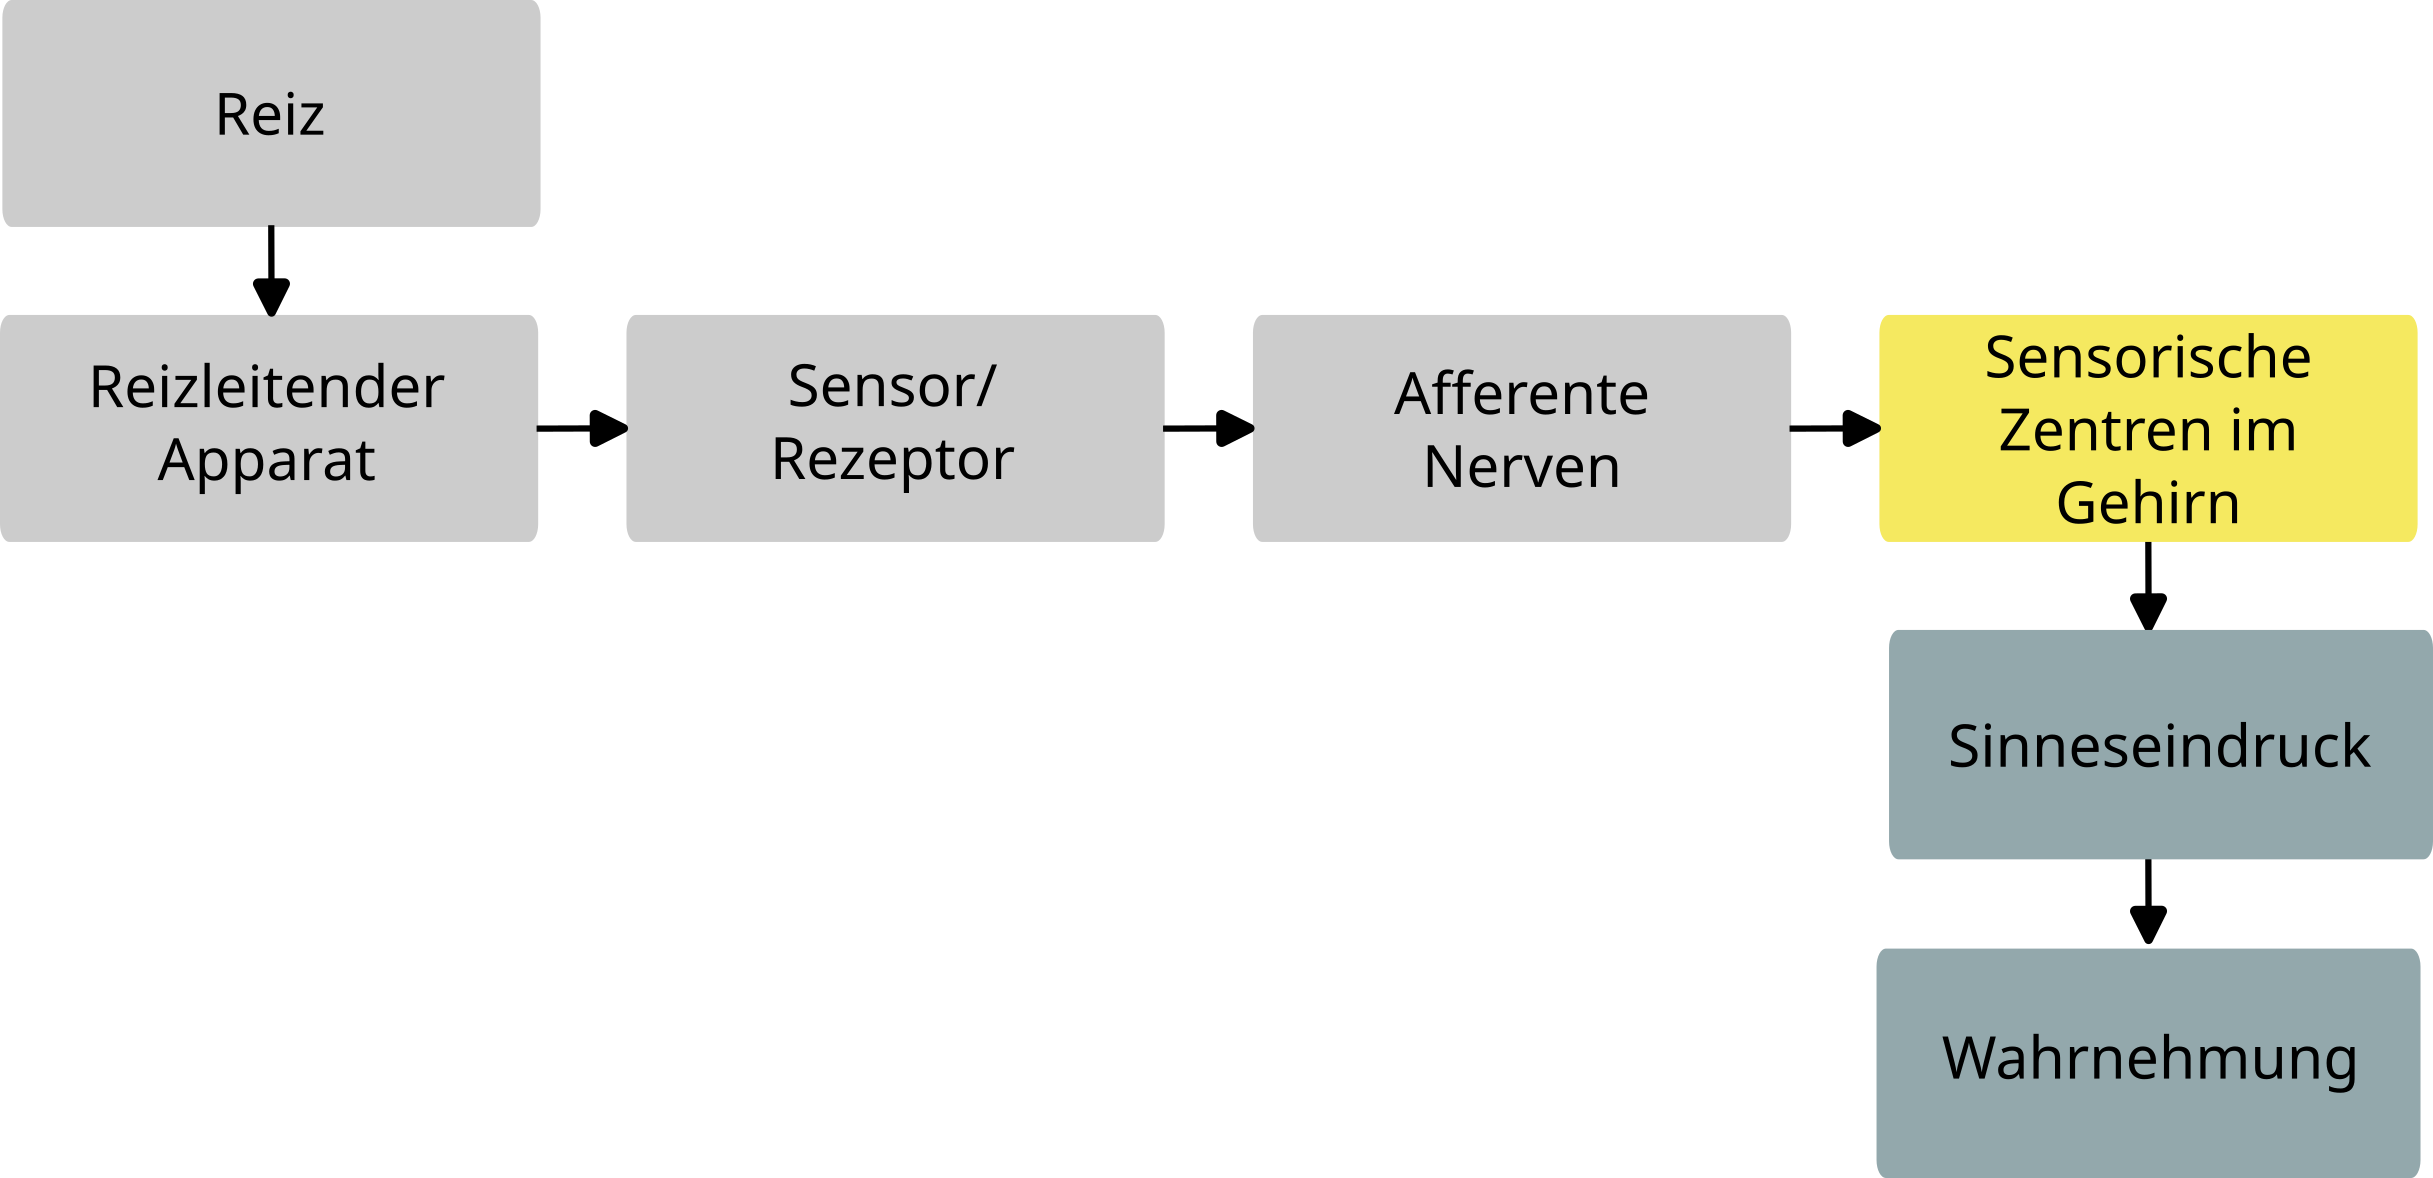
\includegraphics[width=\textwidth]{wahrnehmungsprozess_ohne_beispiel_gehirn.png}
    \end{center}
    
\end{frame}


%%%%%%%%%%%%%%%%%%%%%%%%%%%%%%%%%%%%%%%%%
%%%%  Gehirnregionen und Funktion
%%%%%%%%%%%%%%%%%%%%%%%%%%%%%%%%%%%%%%%%%

    %% sehrinde
\begin{frame}{Primäre Sehrinde}

\begin{columns}[c]

\begin{column}{6cm}
\begin{itemize}
    \item 
    Retinotop organisiert (Fovea centralis nimmt vergleichsweise viel Raum ein)
    \item
    Neurone mit komplexeren rezeptiven Feldern (z.B. selektiv für Orientierung, Bewegungsrichtung, Farbe)
    \item
    Ventrale und dorsale Projektionen
\end{itemize}

\end{column}

\begin{column}{5cm}
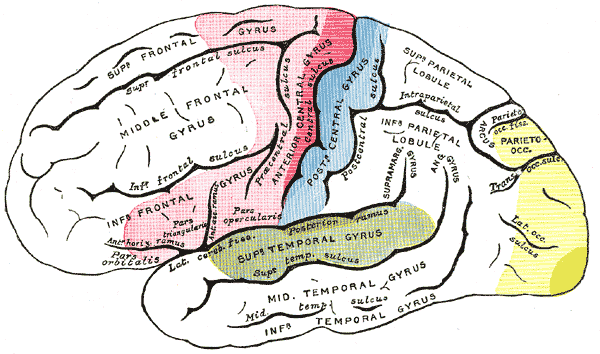
\includegraphics[width=\textwidth]{Gray756.png}
\pause
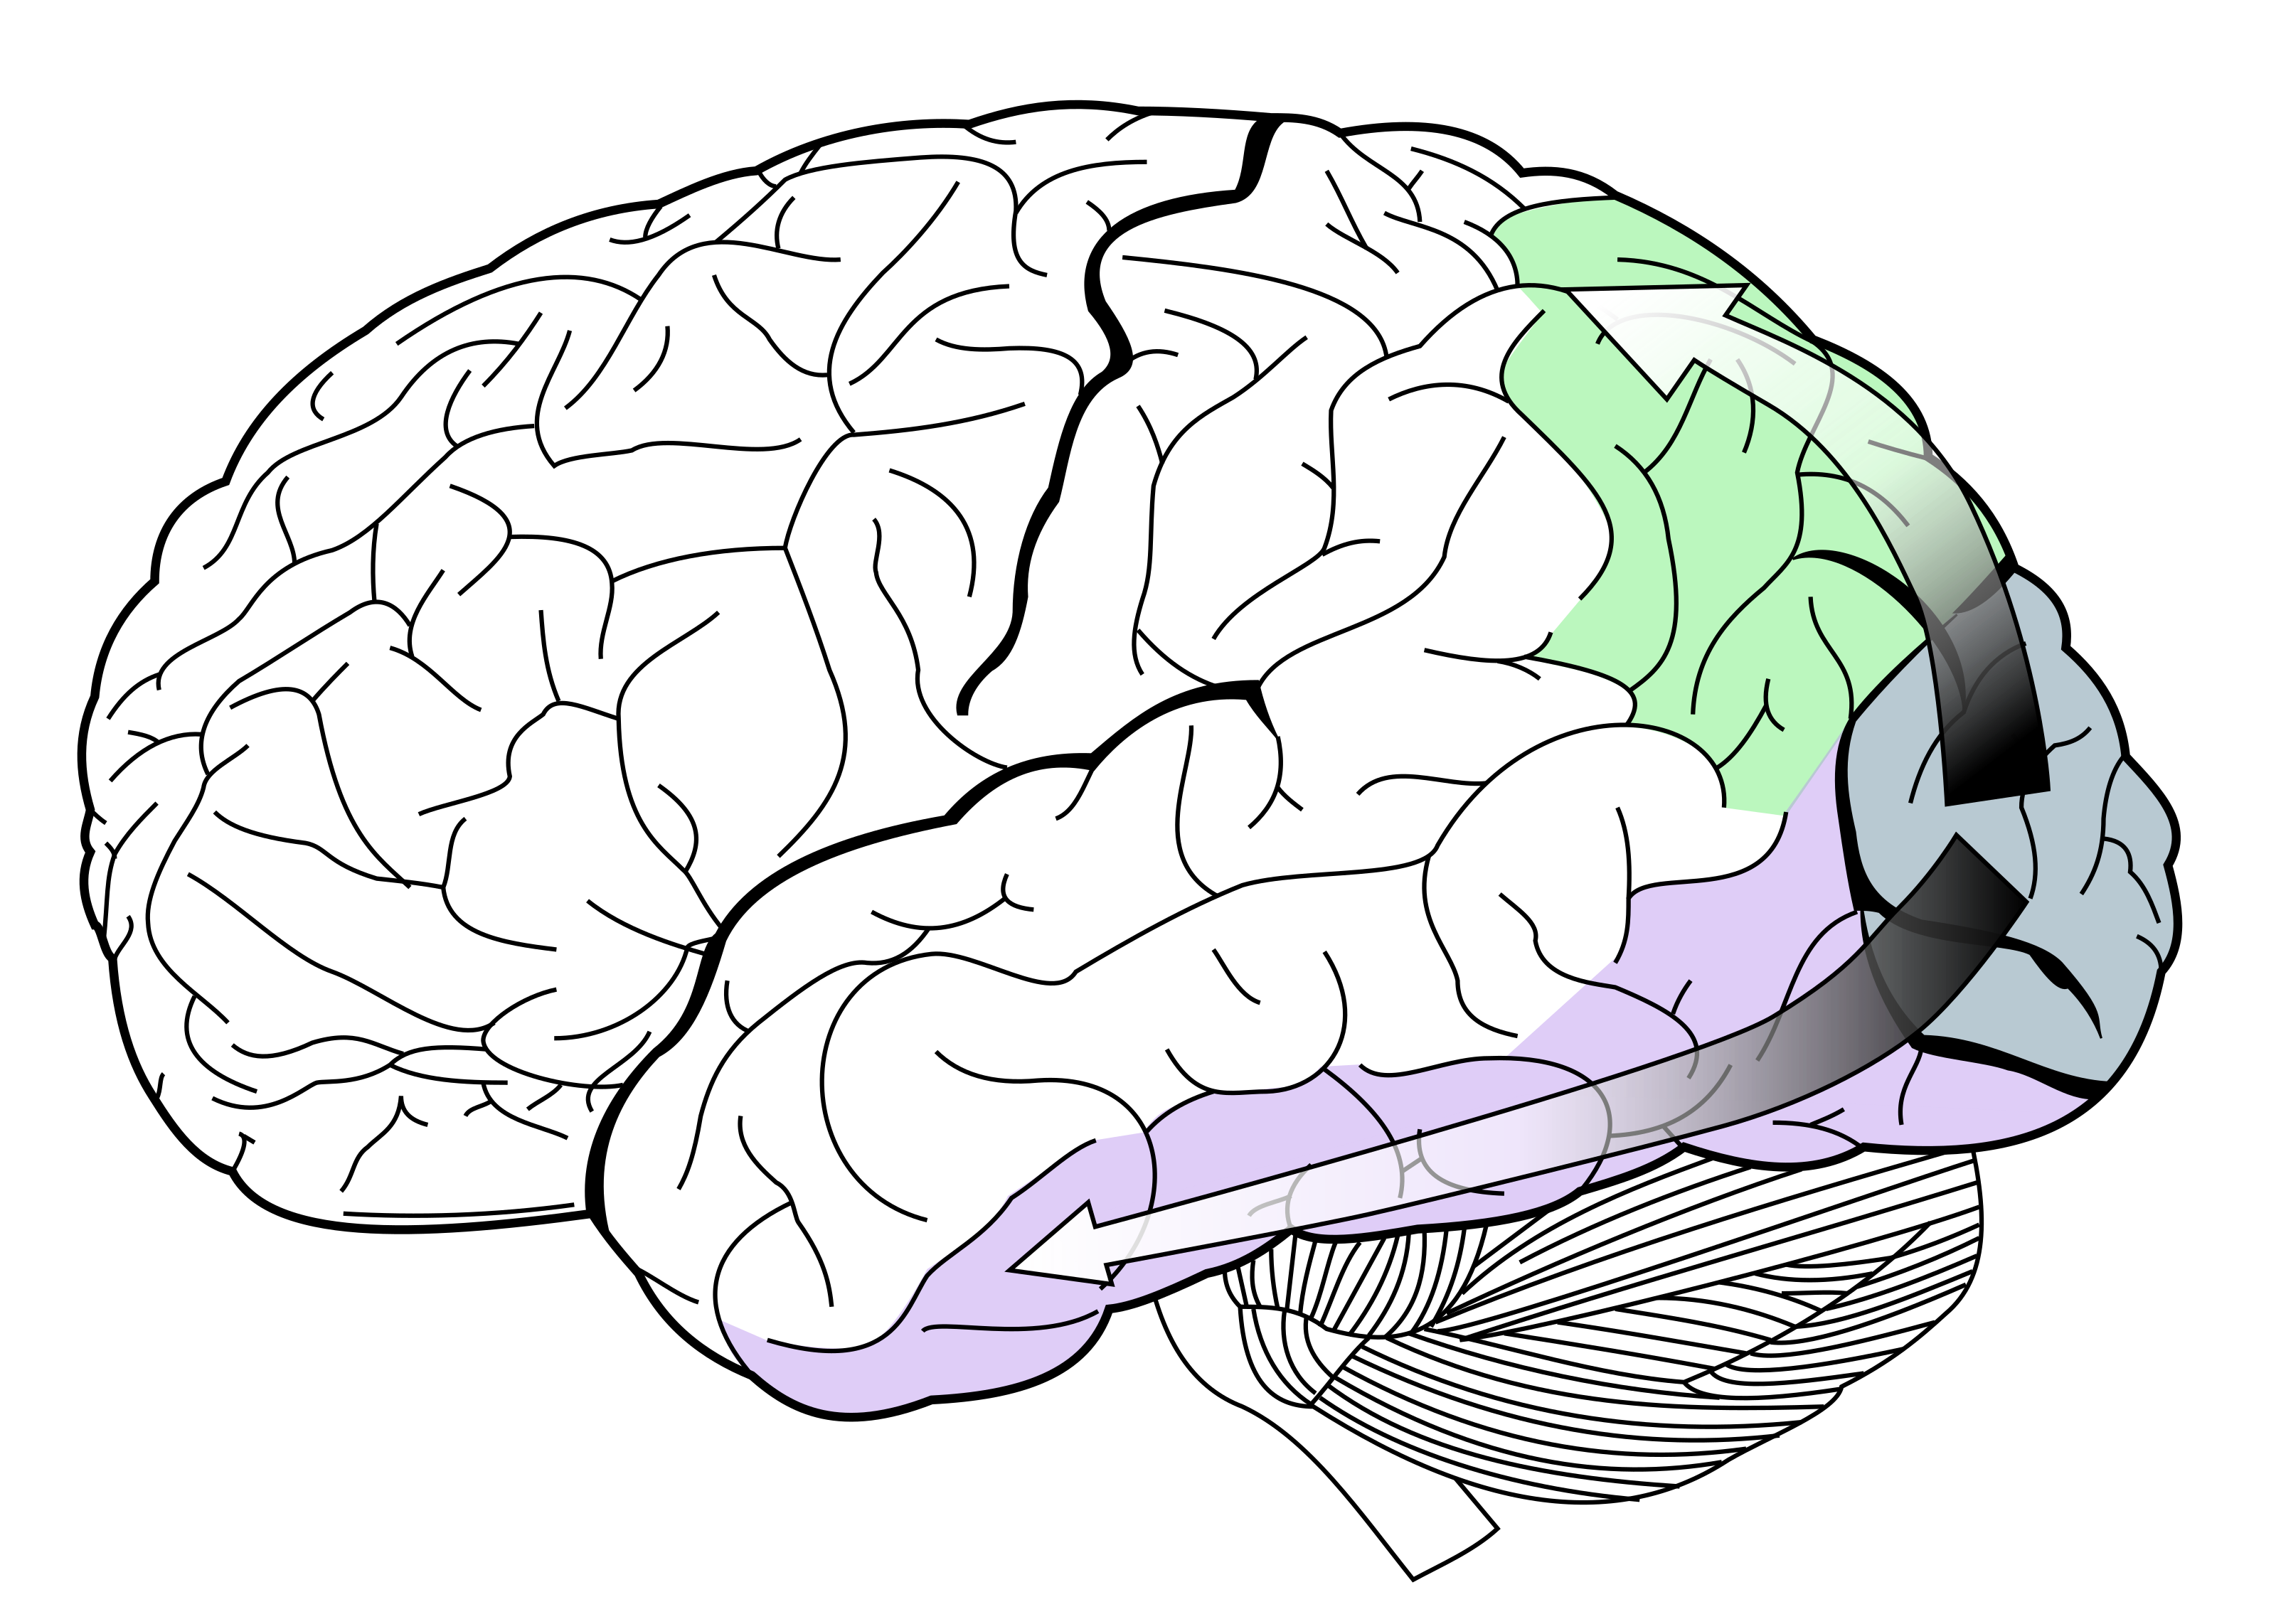
\includegraphics[width=\textwidth]{Ventral-dorsal_streams.png}
\end{column}


\end{columns}
    
\end{frame}
    
    
%% Ventrale Projektionen aus V1
\begin{frame}{Ventrale Projektionen aus V1: "Was?"}

\begin{itemize}
    \item 
    ventraler Teil von V3 \(\rightarrow\) lateraler okzipitaler und inferotemporaler Kortex \(\rightarrow\) entorhinaler Kortex \(\rightarrow\) Hippocampus, limbisches System 
    \item
    Erkennung von Gesichtern, Objekten und Orten
\end{itemize}



    
    
\end{frame}
    
%% Dorsale Projektionen aus V1
    
\begin{frame}{Dorsale Projektionen aus V1: "Wo? Wie?"}

\begin{itemize}
    \item 
    dorsaler Teil von V3 \(\rightarrow\)  mediotemporaler und parietaler Kortex \(\rightarrow\) prämotorischer Kortex \(\rightarrow\) frontales Augenfeld
\item 
    Detaillierte Kartierung des Gesichtsfeldes, Detektion von Bewegung
        \item
    Räumliche Vorstellung und Ausführung von Bewegungen im Raum 
    
\end{itemize}

\end{frame}



%%%%%%%%%%%%%%%%%%%%%%%%%%%%%%%%%%%%%%%%%
%% Efferente Bahnen
%%%%%%%%%%%%%%%%%%%%%%%%%%%%%%%%%%%%%%%%%
\begin{frame}{Efferente Bahnen: Augenbewegungen}

\begin{itemize}
    \item 
    Pupillenreflex
    \item
    Akkommodation
    \item
    Vestibulo-Okulärer Reflex 
    \item
    Folgen einer Bewegung
    \item
    Sakkaden
\end{itemize}


\begin{center}
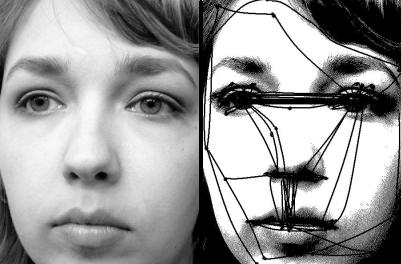
\includegraphics[width=0.6\textwidth]{Szakkad.jpg}
\end{center}

\end{frame}



%%%%%%%%%%%%%%%%%%%%%%%%%%%%%%%%%%%%%%%%%
%% Tiefensehen
%%%%%%%%%%%%%%%%%%%%%%%%%%%%%%%%%%%%%%%%%

\begin{frame}{Beispiel: Tiefensehen}

Wie sehen wir eigentlich in 3D? 

\begin{center}
    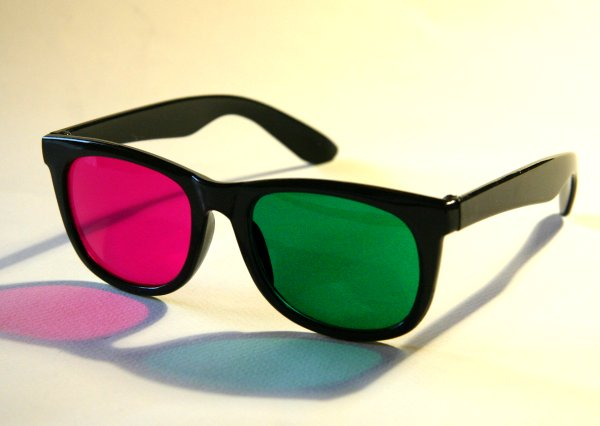
\includegraphics[width=0.8\textwidth]{Green-Magenta-Glasses.jpg}
\end{center}
    
\end{frame}


\begin{frame}{Beispiel: Tiefensehen}

Tiefensehen beruht auf mehreren Strategien:

\begin{itemize}
    \item 
    Geometrische Unterschiede zwischen der Darstellung eines Objektes in beiden Augen
    \item
    Parallaxenunterschiede
    \item
    Erfahrungswissen darüber, wie groß Objekte sind und wie sie aus der Entfernung kleiner erscheinen
    \item
    Ordnung von Objekten nach Verdeckungseigenschaften
    \item
    Bewegung der Augenmuskeln dergestalt, dass beide Augen auf dasselbe Objekt fokussieren. Ist das nicht möglich (z.B. bei Strabismus), dann kann es sein, dass das Objekt doppelt gesehen wird (Diplopie)
\end{itemize}



\end{frame}






%% %% %% %% Review


\begin{frame}

 \frametitle{Jetzt* sollten Sie folgendes können}



\begin{block}{Grundlagen:}




\begin{itemize}

    \item 
den Aufbau der Retina beschreiben
    \item 
die Rolle des Pigmentepithels erläutern
    \item 
die molekularen und zellulären Grundlagen der Photorezeption erläutern
    \item 
photopisches und skotopisches Sehen beschreiben und erklären
    \item 
die Physiologie des Farbsehens beschreiben
    \item 
die Anatomie der Sehbahn beschreiben
    \item 
die Rolle von kortikalen Regionen beim Sehen beschreiben
    \item 
die Rolle efferenter Verbindungen beim Sehen erläutern
    \item 
die Grundlagen des Tiefensehens erklären
\end{itemize}


\end{block}

\end{frame}

\begin{frame}

 \frametitle{Jetzt* sollten Sie folgendes können}

 

\begin{block}{Klinik:}

\begin{itemize}
    
\item 
Anomalien im Farbsehen benennen und erklären
    \item 
Perimetrie beschreiben und Anwendungen erklären
    \item 
Ausfälle des Gesichtsfeldes erklären und beschreiben
    \item 
Diplopie definieren und erklären
    \item 
Strabismus definieren und erklären

\end{itemize}


\end{block}



\end{frame}





%% Feedbackhinweisblock
\begin{frame}
\frametitle{Danke für Ihr Feedback!}


\begin{center}

\includegraphics[width=0.7\textwidth]{feedback_QR.png}
\end{center}
\end{frame}




%% %% %% Bildnachweis


\begin{frame}
\frametitle{Bildnachweis}
\begin{tiny}



 
\begin{itemize}

\item
Architektonische Struktur in bunten Farben. Photo by \href{https://unsplash.com/@ro_ka?utm_source=unsplash&utm_medium=referral&utm_content=creditCopyText}{Robert Katzki} on \href{https://unsplash.com/?utm_source=unsplash&utm_medium=referral&utm_content=creditCopyText}{Unsplash}
  

\item
3D-Brille. Von Oliver Olschewski aus 3D-Foto-Shop, CC BY-SA 3.0 de, \url{https://commons.wikimedia.org/w/index.php?curid=16036543}

\item
Absorptionskurven für Stäbchen- und Zapfenzellen. Modifiziert von mir (Farbe geändert, um für Farebenblinde besser lesbar zu sein; Buchstaben-Bezeichnungen modifiziert). Vorlage von Cone-response.svg: w:User:DrBob and w:User:Zeimusuderivative work: Sgbeer - Cone-response.svg (Vectorized version of the GFDL image Cone-response.png uploaded by User:Maxim Razin based on work by w:User:DrBob and w:User:Zeimusu.), CC BY-SA 3.0, \url{https://commons.wikimedia.org/w/index.php?curid=17729332}

\item
Aktivierungsmuster von On- und Off-Bipolarzellen und On- und Off-Ganglienzellen. Cristiane Tilelli, CC BY-SA 4.0 \url{https://creativecommons.org/licenses/by-sa/4.0}, via Wikimedia Commons

\item
Aufbau von Stäbchen und Zapfen. Meine Übersetzung aus dem Französichen von Pancrat, CC BY-SA 3.0 \url{https://creativecommons.org/licenses/by-sa/3.0}, via Wikimedia Commons

\item
Ausfälle im Gesichtsfeld bei Schäden entlang der Sehbahn. Von mir verändert (Gesichtsfelder unterschidelich eingefärbt) nach Albert Kok at Dutch Wikipedia, Public domain, via Wikimedia Commons. 
 
\item
Diagramm mit mehreren Farben und wie es sich für Menschen mit Schwaächen im Farbsehen darstellt. By Grolltech - Own work, CC BY-SA 3.0, \url{https://commons.wikimedia.org/w/index.php?curid=22912023}


\item
Dunkeladaptation als eine Funktion der Zeit. Von Anton - painting of diagram: own work. Data: collected from different sources and averaged., Gemeinfrei, \url{https://commons.wikimedia.org/w/index.php?curid=2583079}

\item
Fundusfotografie einer Retina. Häggström, Mikael (2014). "Medical gallery of Mikael Häggström 2014";. WikiJournal of Medicine 1 (2). DOI:10.15347/wjm/2014.008. ISSN 2002-4436. Public Domain. \url{https://commons.wikimedia.org/w/index.php?curid=18776091}
   
   \item
Fundusfotografie einer Retina mit eingezeichneten Strukturen. Von Photograph: Danny Hope from Brighton \& Hove, UK, Diagram: User:Zyxwv99 - Photograph: File:Righ\_eye\_retina.jpg (which come from My Right Eye)Diagram: Eigenes Werk ( User:Zyxwv99 ), CC BY 2.0,\url{ https://commons.wikimedia.org/w/index.php?curid=36685094}
  
  
 \item
 
 Gesichtsfeld eines rechten Auges. Pignol23, CC BY 3.0 \url{https://creativecommons.org/licenses/by/3.0}, via Wikimedia Commons
 \end{itemize}
\end{tiny}
\end{frame}

 
\begin{frame}
\frametitle{Bildnachweis}
\begin{tiny}



 
\begin{itemize}

  
\item
Korrektur von Kurzsichtigkeit mithilfe einer Streulinse. By Gumenyuk I.S. - Own work, CC BY-SA 4.0, \url{https://commons.wikimedia.org/w/index.php?curid=46820576}


\item
Opsin- und Retinalzyklus. By OpenStax College - Anatomy &amp; Physiology, Connexions Web site. \url{http://cnx.org/content/col11496/1.6/}, Jun 19, 2013., CC BY 3.0, \url{https://commons.wikimedia.org/w/index.php?curid=30148001}

\item
Perimetrische Untersuchung. Sej994, CC BY-SA 4.0 \url{https://creativecommons.org/licenses/by-sa/4.0}, via Wikimedia Commons


\item
Phototransduktion. Jason J. Corneveaux, wiki user: Caddymob, CC BY 3.0 \url{https://creativecommons.org/licenses/by/3.0}, via Wikimedia Commons

\item
Regionen des Cortex (die Sehrinde ist in gelb eingezeichnet). Von Henry Vandyke Carter - Henry Gray (1918) Anatomy of the Human Body (See "Buch" section below)Bartleby.com: Gray's Anatomy, Tafel 756, Gemeinfrei, \url{https://commons.wikimedia.org/w/index.php?curid=541602}

\item
Sakkaden. Original file: SpooSpa. Derivative: Simon Viktória, CC BY-SA 2.0 \url{https://creativecommons.org/licenses/by-sa/2.0}, via Wikimedia Commons

\item
Sehbahn mit Chiasma Opticum, detailliert. KDS444, CC BY-SA 4.0 \url{https://creativecommons.org/licenses/by-sa/4.0}, via Wikimedia Commons

\item
Sehbahn mit farblicher Darstellung des linken und rechten Gesichtsfeldes. JonRichfield, CC BY-SA 4.0 \url{tps://creativecommons.org/licenses/by-sa/4.0}, via Wikimedia Commons

\item
Ventrale und dorsale Projektionen aus V1. By Selket - I (Selket) made this from File:Gray728.svg, CC BY-SA 3.0, \url{https://commons.wikimedia.org/w/index.php?curid=1679336}

\item
Verteilung von Stäbchen und Zapfen in der Retina. Von Cmglee - Eigenes Werk, CC BY-SA 3.0, \url{https://commons.wikimedia.org/w/index.php?curid=29924570}

\item
Wahrnehmungsbahn und einzelne Prozesse entlang der Wahrnehmungsbahn (mehrere Bilder). Mein eigenes Werk, CC BY-SA 4.0, 2022. 

\item
Zellen der Retina. Modifiziert von mir, CC BY-SA 4.0, 2022, nach einer Vorlage von  Pancrat, CC BY-SA 4.0 \url{https://creativecommons.org/licenses/by-sa/4.0}, via Wikimedia Commons

\end{itemize}
\end{tiny}
\end{frame}






\end{document}

%%% Frequently used snippets

%% \begin{columns}[c]

%% \begin{column}{5cm}
%% \end{column}

%% \begin{column}{5cm}
%% \end{column}


%% \end{columns}




